% !BIB program = biber 
\documentclass{article}

%% Encoding
\usepackage[T1]{fontenc}
\usepackage[utf8]{inputenc}

%% Fonts
% Math fonts (fourier) with utopia (erewhon) text fonts
\usepackage{fourier, erewhon}
\usepackage{algorithm}
\usepackage[noend]{algpseudocode}

%% Setup
% This package contains logos
\usepackage[autoload]{adn}

\setlogos[
\textbf{MO435 --- Probabilistic Machine Learning}\\%[5pt]
\uppercase{Instituto de Computação --- UNICAMP}\\%[-7pt]
]%
{IC3D}%
{UNICAMP}

%% Transform section references
\makeatletter
\renewcommand*{\p@section}{\S\,}
\renewcommand*{\p@subsection}{\S\,}
\makeatother

%% Shorthands
\usepackage{xspace}
\makeatletter
\DeclareRobustCommand\onedot{\futurelet\@let@token\@onedot}
\def\@onedot{\ifx\@let@token.\else.\null\fi\xspace}

\def\eg{e.g\onedot} \def\Eg{E.g\onedot}
\def\ie{i.e\onedot} \def\Ie{I.e\onedot}
\def\cf{cf\onedot} \def\Cf{Cf\onedot}
\def\etc{etc\onedot} \def\vs{vs\onedot}
\def\wrt{w.r.t\onedot} \def\dof{d.o.f\onedot}
\def\etal{et al\onedot}
\makeatother

%%%
% Other packages start here (see the examples below)
%%

%% Figues
\usepackage{graphicx}
\graphicspath{{../output/}}
\usepackage{caption}
\usepackage{subcaption}
\usepackage{array}
\usepackage{multirow}

%% References
% Use this section to embed your bibliography
% Instead of having a separate file, just place the bibtex entries here
\usepackage{filecontents}% create files
\begin{filecontents}{\jobname.bib}
  @article{sathya2013,
    doi = {10.14569/ijarai.2013.020206},
    year = {2013},
    publisher = {The Science and Information Organization},
    volume = {2},
    number = {2},
    author = {R. Sathya and Annamma Abraham},
    title = {Comparison of Supervised and Unsupervised Learning Algorithms for Pattern Classification},
    journal = {International Journal of Advanced Research in Artificial Intelligence}
  }
  @book{bishop2006,
    author = {Bishop, Christopher M.},
    edition = 1,
    isbn = {0-387-31073-8},
    publisher = {Springer},
    title = {Pattern Recognition and Machine Learning},
    year = 2006
  }
  @book{murphy2012,
  title={Machine Learning: A Probabilistic Perspective},
  author={Murphy, Kevin P},
  pages={27--33},
  year={2012},
  publisher={The MIT Press},
  }
\end{filecontents}
% Include bibliography file
\usepackage[
backend=biber, 
style=ieee, 
natbib=true,
]{biblatex}
\addbibresource{\jobname.bib}

%% Math
\usepackage{amsmath}
\DeclareMathOperator{\E}{\mathbb{E}}

%% Enumerate
\usepackage{enumitem}

\begin{document}

% Put the topic of the assignment here
\title{Project 2}
% Put your name here 
\author{
Jo\~ao Victor da Silva Guerra 
and
Leonardo Alves de Melo
\thanks{117410 and 156188. j117410@dac.unicamp.br and leonardo.alves.melo.1995@gmail.com.}
}

\maketitle

\begin{abstract}
In this project, we implemented a Gaussian Processes algorithm, and evaluated it with samples of the sine, cossine and exponential functions. For each function, we evaluated the size of the training set and test set, varying in 5, 10 and 50 samples. In addition, our implementation was able to evaluate higher dimensional data, which we illustrated with a two-dimensional data. Finally, we evaluated the effects of the  squared-exponential kernel parameters and different kernel functions on our predictions.
\end{abstract}

\section{Introduction}

A Bayesian Optmization ia a way to find the global maximun or minimun of a given function without calculating the derivative. The Gaussian Processes (GP) is a type of Bayesian Optmization, and performs a Bayesian inference over the functions. In this approach, the prior is defined over functions and, after seen some data, it can be used to find the porterior, which is a distribution over some arbitrary set of points of a function (\cite{murphy2012}).

Given a set of points $ x_1, ..., x_n $, the objective is to calculate the corresponding $ f(x_1), ..., f(x_n) $. A GP assumes that $ p(f(x_1), ..., f(x_n)) $ is a jointly Gaussian distribution, with some mean $\mu(x)$ and covariance $\Sigma(x)$. To get the covariance values, we have to define a positive definite kernel function $\kappa(x_i, x_j)$ as follows:

\begin{equation}
  \Sigma_{ij} = \kappa(x_i, x_j)
  \label{eq:covariance}
\end{equation}

\subsection{Gaussian Processes for regression}

In a GP regression, we assume that the prior on the regression function is a GP (Eq. \eqref{eq:gpr_prior}) with a mean function $m(x)$ (Eq. \eqref{eq:m_prior}) and a kernel function $\kappa(x,x')$ (Eq. \eqref{eq:cov_prior}). 

\begin{equation}
  f(x) \sim GP(m(x), k(x,x'))
  \label{eq:gpr_prior}
\end{equation}

\begin{equation}
  m(x) = \E[f(x)]
  \label{eq:m_prior}
\end{equation}

\begin{equation}
  \kappa(x,x') = \E[(f(x) - m(x))(f(x') - m(x'))^T]
  \label{eq:cov_prior}
\end{equation}

For a finite set of points, this process becomes a joint Gaussian distribution as follows: 

\begin{equation}
  p(f|X) = \mathcal{N}(f|\mu, K)
  \label{eq:jointGaussian}
\end{equation}
where $K_{ij} = \kappa(x_i, x_j)$ and $\mu = (m(x_1), ..., m(x_n))$.

Now, suppose we have a training set ($D = {(x_i, y_i), i = 1:N)}$), where $y_i$ is a noisy observation at $x_i$, yielded by $y = f(x) + \epsilon$, where $\epsilon \sim \mathcal{N}(0, \sigma_y^2)$. Further, given a test set $X_*$ of size $N_* \times D$, we want predict the function outputs $f_*$. As we have noisy observations, our model must come "close", but is not necessary to interpolate the data.

The joint distribution of the observed data and the latent noise-free function is given by

\begin{equation}
  \begin{pmatrix}
      y \\ 
      f_*
  \end{pmatrix}
  \sim \mathcal{N}
  \begin{pmatrix}
  0, & \begin{pmatrix} K_y & K_* \\ K_*^T & K_{**} \end{pmatrix}
  \end{pmatrix}
\end{equation}
where $K_y = \kappa(X, X) + \sigma_y^2I_N$ is $N \times N$,
$K_* = \kappa(X, X_*)$ is $N \times N_*$, and $K_{**} = \kappa(X_*, X_*)$ is $N_* \times N_*$. The second term of the covariance of the noisy observation ($\sigma_y^2I_N$) is a diagonal because the noise term ($\sigma_y^2$) is independently added to each observation. 

According to standard rules for conditioning Gaussian distributions (\cite{murphy2012}), the posterior has the form

\begin{equation}
p(f_*|X_*, X, y) = \mathcal{N}(f_*|\mu_*, \Sigma_*)
\end{equation}

\begin{equation}
  \mu_* = K_*^T K_y^{-1} y
\end{equation}

\begin{equation}
  \Sigma_* = K_{**} - K_*^T K_y^{-1} K_*
\end{equation}

Here, we implement a Gaussian Process regression and evaluate the effect of the model parameters, such as samples from different function, training and test set sizes, noise's standard deviation, kernel parameters, kernel functions, on the predictions (\ie posterior).

% will test an algorithm for Gaussian Processes using the Squared-Exponential kernel given by Equation \ref{eq:kernel}, where $\sigma$ and $\ell$ are parameters of the kernel, and for this project will be set as equal to 1.0. The algorithm will be evaluated for different amounts of samples, three different functions and for other kernels.

% \begin{equation}
%   k_{SE}(x,x') = \sigma^2e^{-\frac{(x-x')^2}{2\ell^2}}  
%   \label{eq:kernel}
% \end{equation}

\section{Algorithm}

The predictive mean is calculated by the Eq.\eqref{eq:predictiveMean}. However, the direct computation of $K^{-1}_y$ is not recommended because of numerical stabilities. Therefore, an alternative approach is to compute the Cholesky decomposition of $K_y$, which is given by Eq.\eqref{eq:cholesky}. 

\begin{equation}
  \overline{f_*} = K^T_*K^{-1}_yy
  \label{eq:predictiveMean}
\end{equation}

\begin{equation}
  K_y = LL^T
  \label{eq:cholesky}
\end{equation}

Then, we compute the predictive mean, variance and the log marginal likelihood, using Cholesky decomposition, as shown in Algorithm \ref{algo:gp}.

\begin{algorithm}
  \caption{Gaussian Processes Regression}
  \label{algo:gp}
  \begin{algorithmic}[1]
      \State $L = cholesky(K + \sigma^2_yI);$
      \State $\alpha = L^T\textbackslash(L\textbackslash y);$
      \State $\mathbb{E}[f_*] = K^T_*\alpha;$
      \State $v = L\textbackslash K_*;$
      \State $var[f_*] = \kappa(x_*,x_*) - v^Tv;$
      \State $log(p(y|X)) = -\frac{1}{2}y^T\alpha - \Sigma_ilogL_{ii} - \frac{N}{2}log(2\pi);$
  \end{algorithmic}
\end{algorithm}

\section{Experiments}

\subsection{Data}

For our experiments, we sampled our training and test sets from different functions. For the functions, we selected sine ($f_1$, Eq.\eqref{eq:sin}), cosine ($f_2$, Eq.\eqref{eq:cos}), exponential ($f_3$, Eq.\eqref{eq:exp}) and a 2D periodic function ($f_4$, Eq.\eqref{eq:2d}). All functions are displayed in the range from -5 to 5 on the axes of the independent variables in Fig.\ref{fig:1}.

\begin{equation}
  f_1(x) = sin(\pi x)
  \label{eq:sin}
\end{equation}

\begin{equation}
  f_2(x) = cos(\pi x)
  \label{eq:cos}
\end{equation}

\begin{equation}
  f_3(x) = e^x
  \label{eq:exp}
\end{equation}

\begin{equation}
  f_4(x_1, x_2) = sin(\pi x_1) + cos(\pi x_2)
  \label{eq:2d}
\end{equation}

\begin{figure}[ht]
  \begin{subfigure}{.5\textwidth}
    \centering
    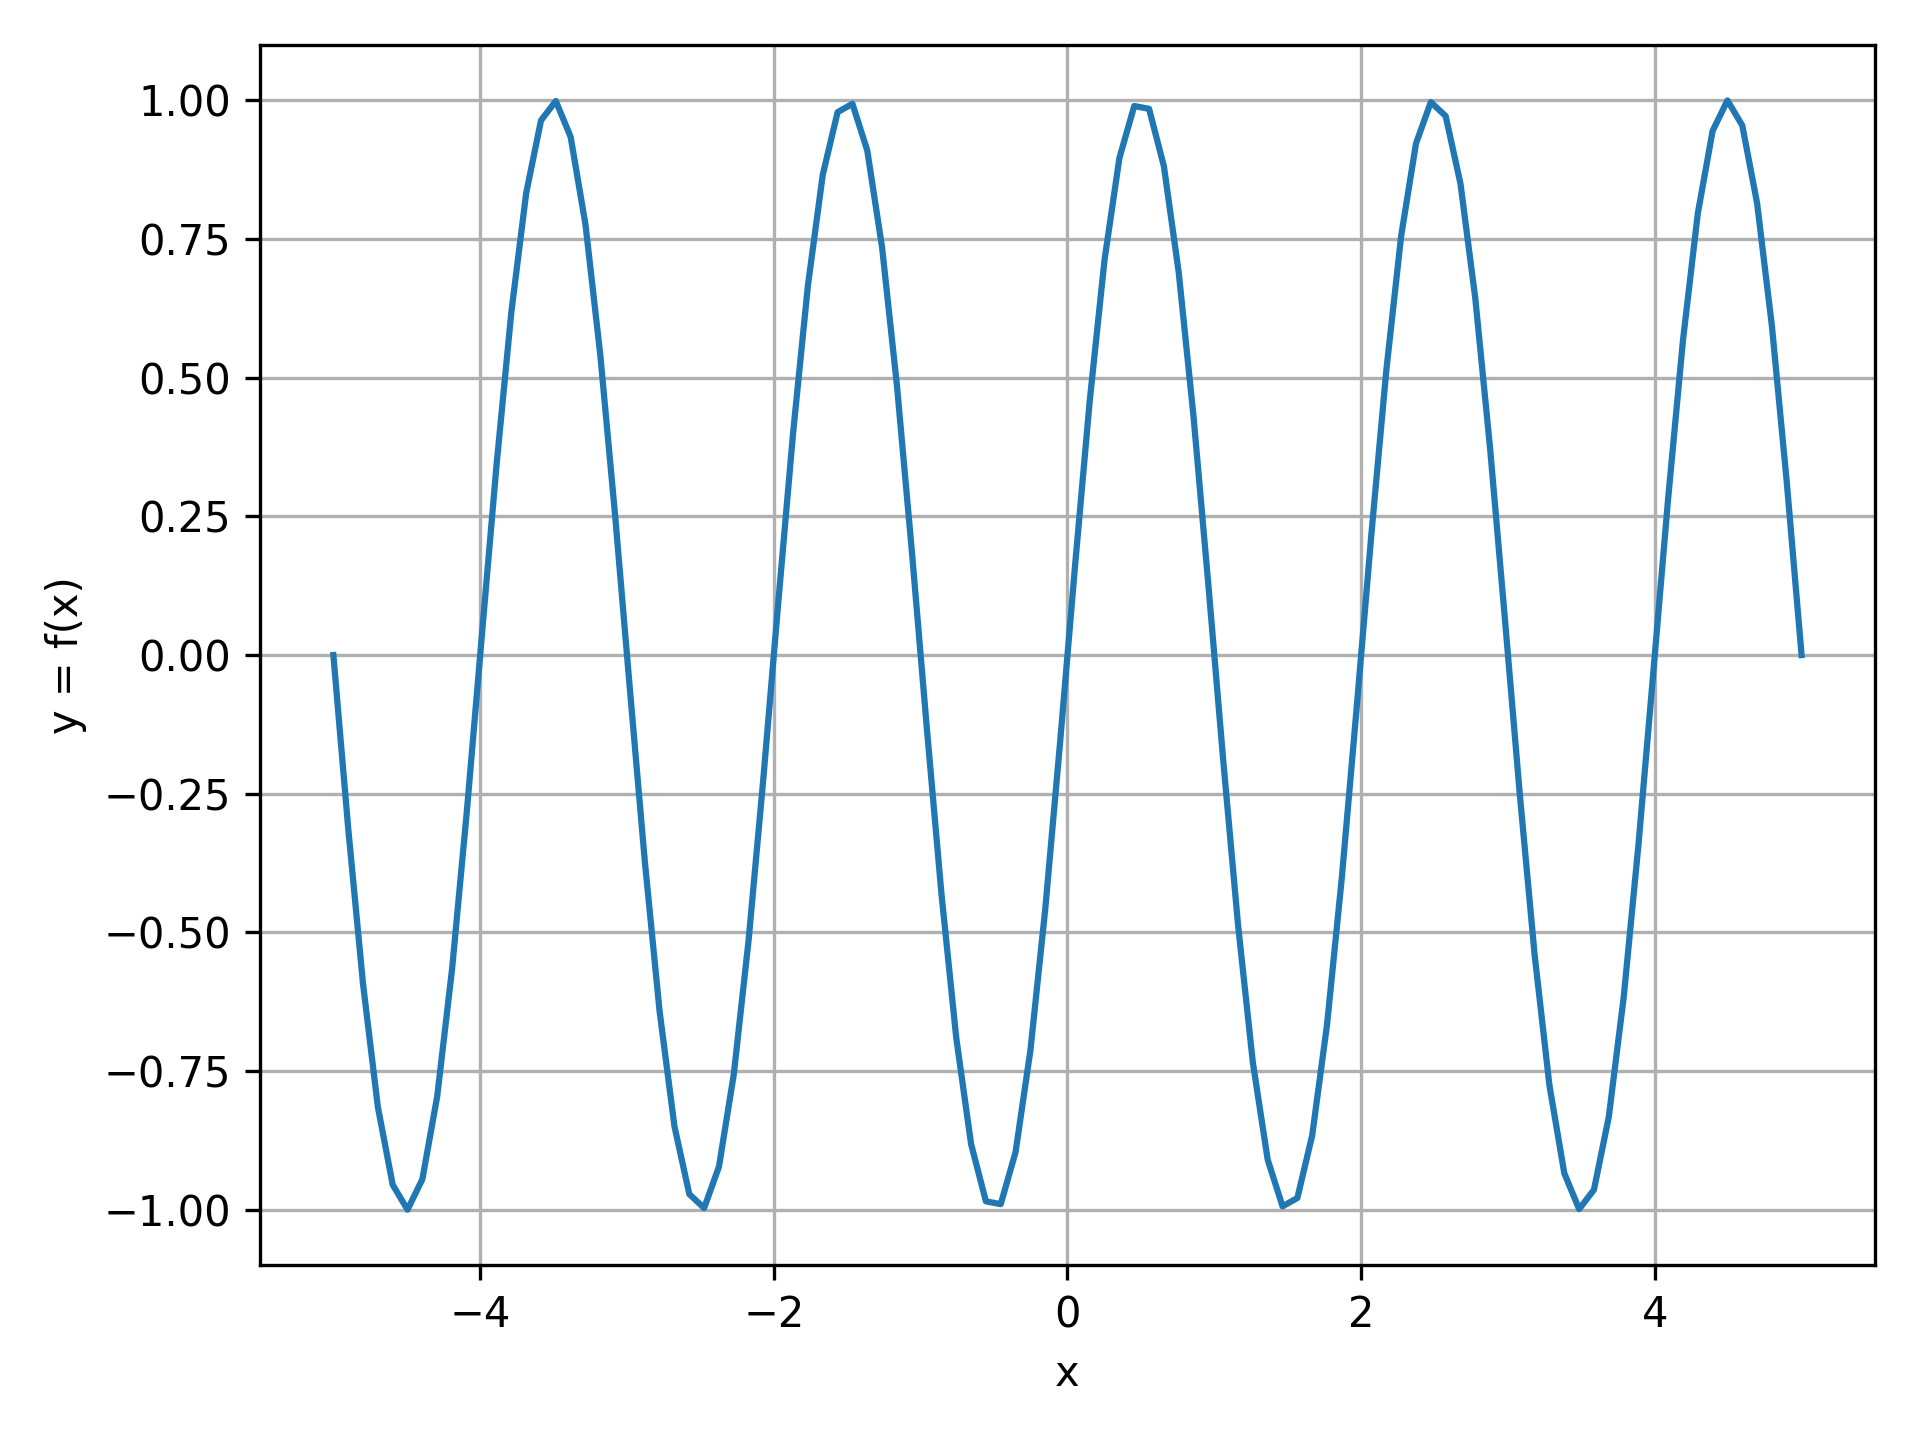
\includegraphics[width=.8\linewidth]{functions/sin.png}
    \caption{Sine function ($f_1$)}
  \end{subfigure}
  \begin{subfigure}{.5\textwidth}
    \centering
    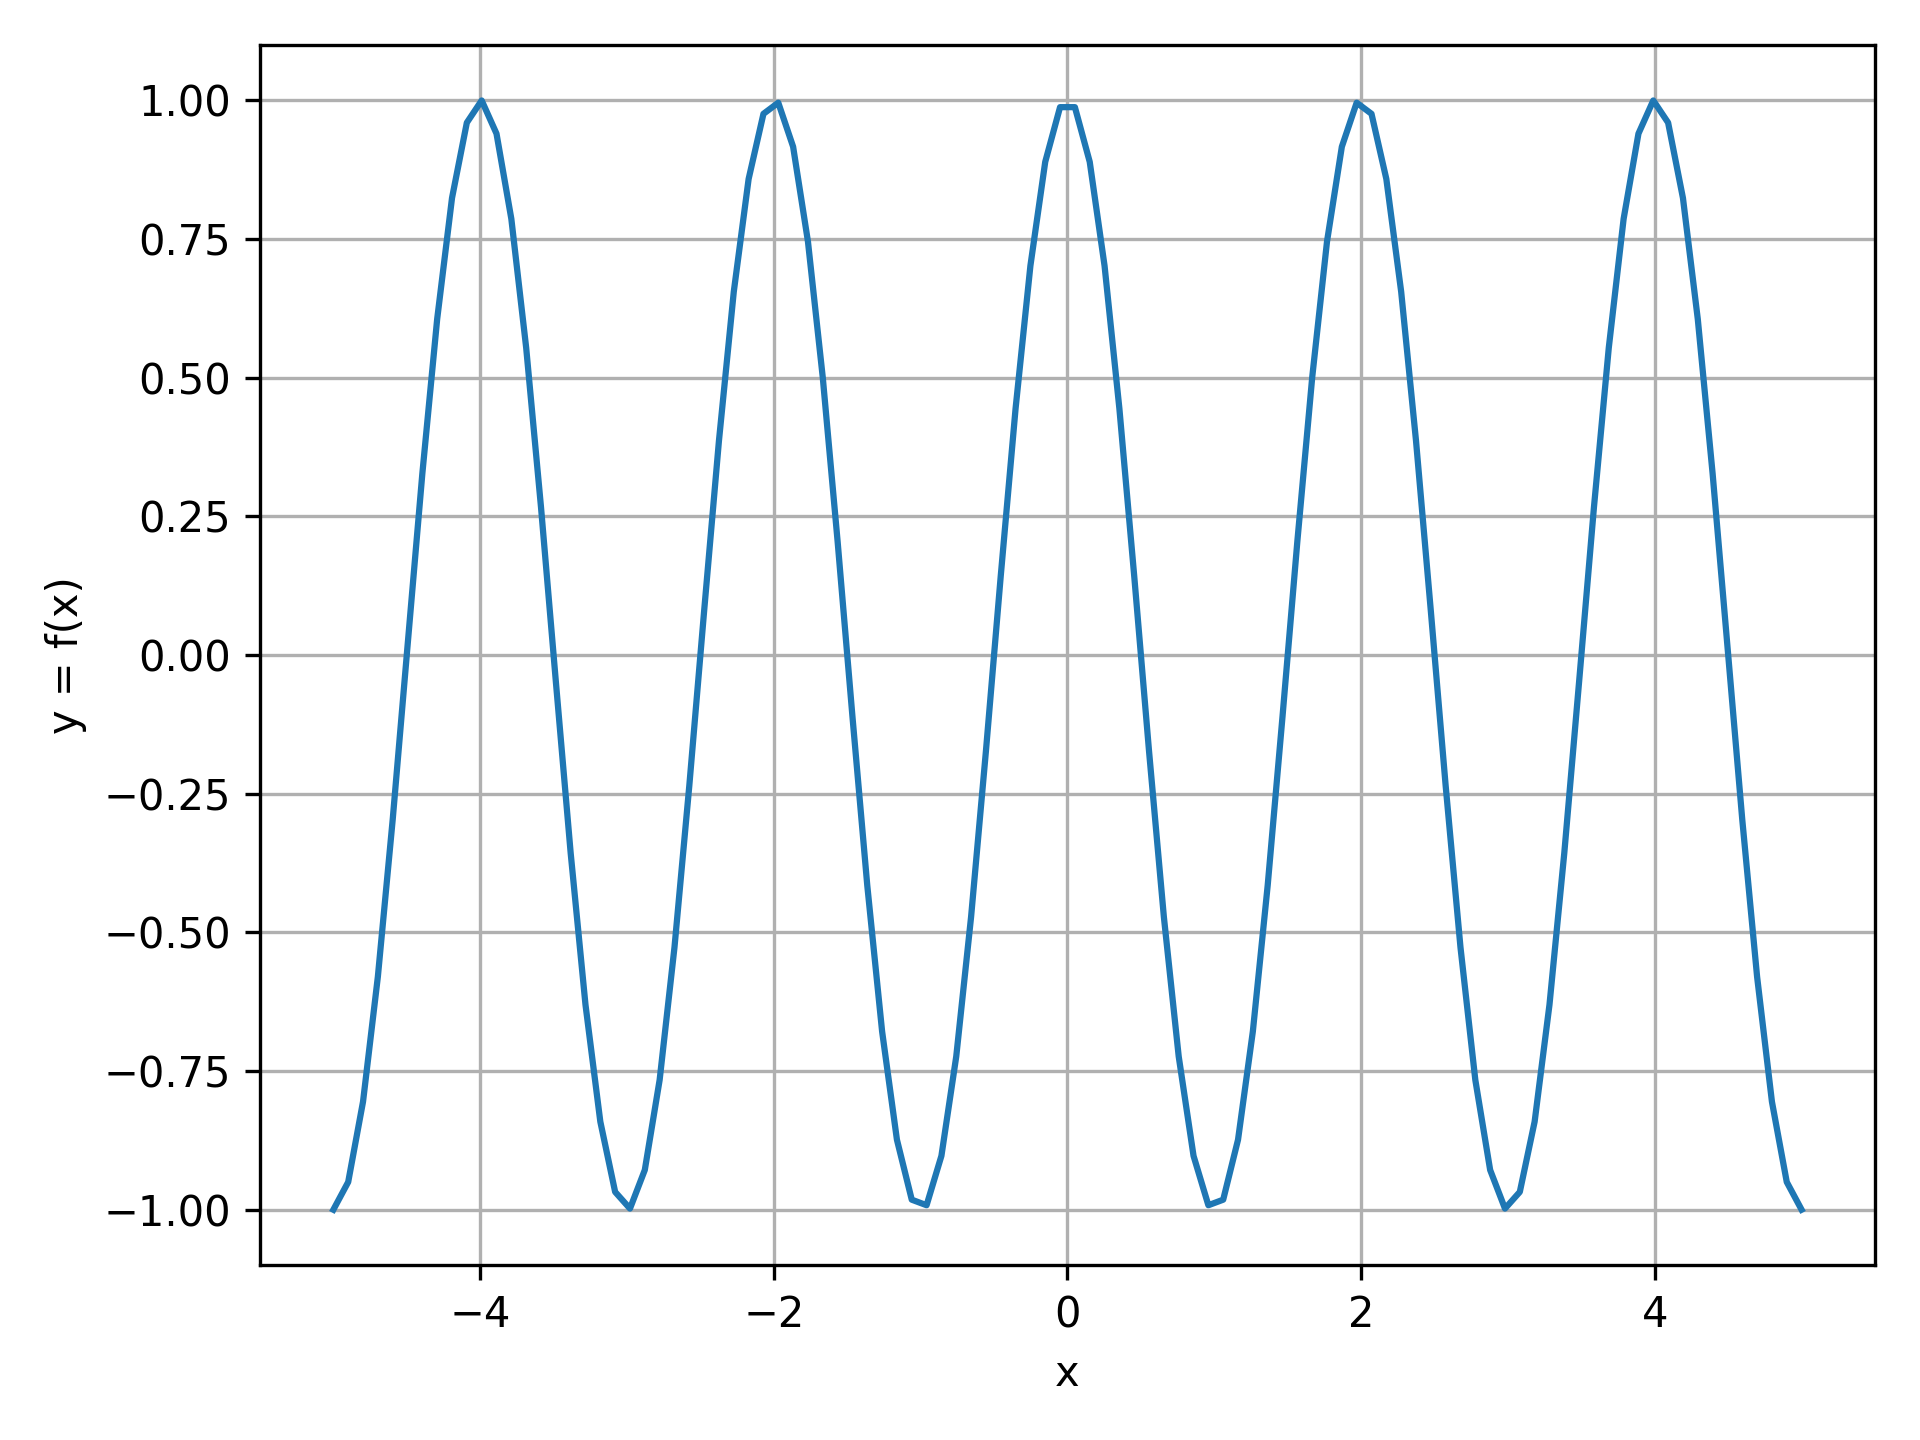
\includegraphics[width=.8\linewidth]{functions/cos.png}
    \caption{Cosine function ($f_2$)}
  \end{subfigure}
  \begin{subfigure}{.5\textwidth}
    \centering
    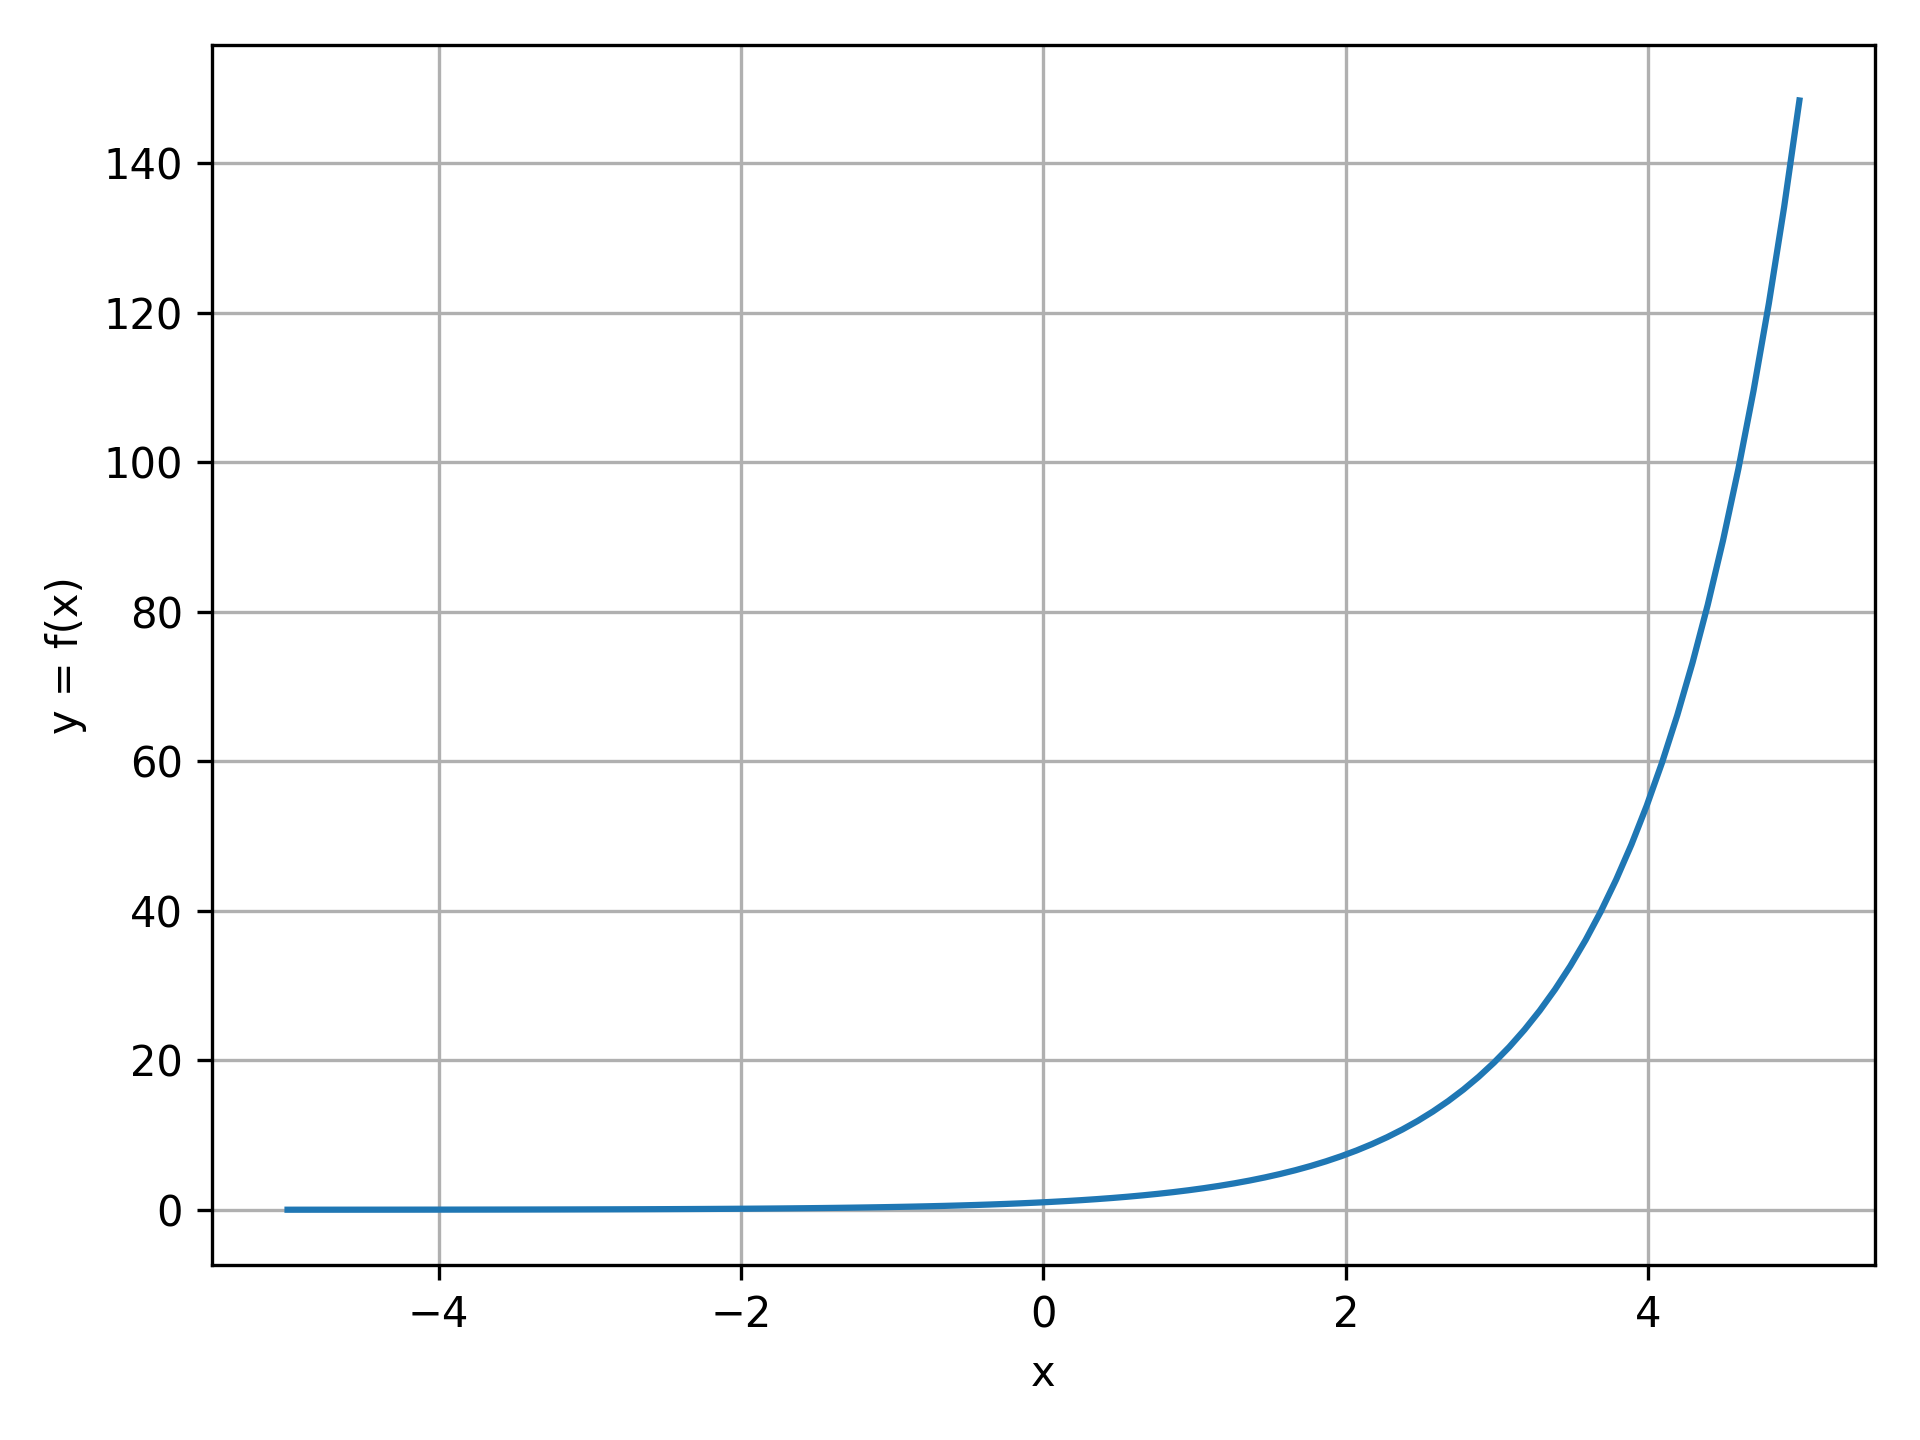
\includegraphics[width=.8\linewidth]{functions/exp.png}
    \caption{Exponential function($f_3$)}
  \end{subfigure}
  \begin{subfigure}{.5\textwidth}
    \centering
    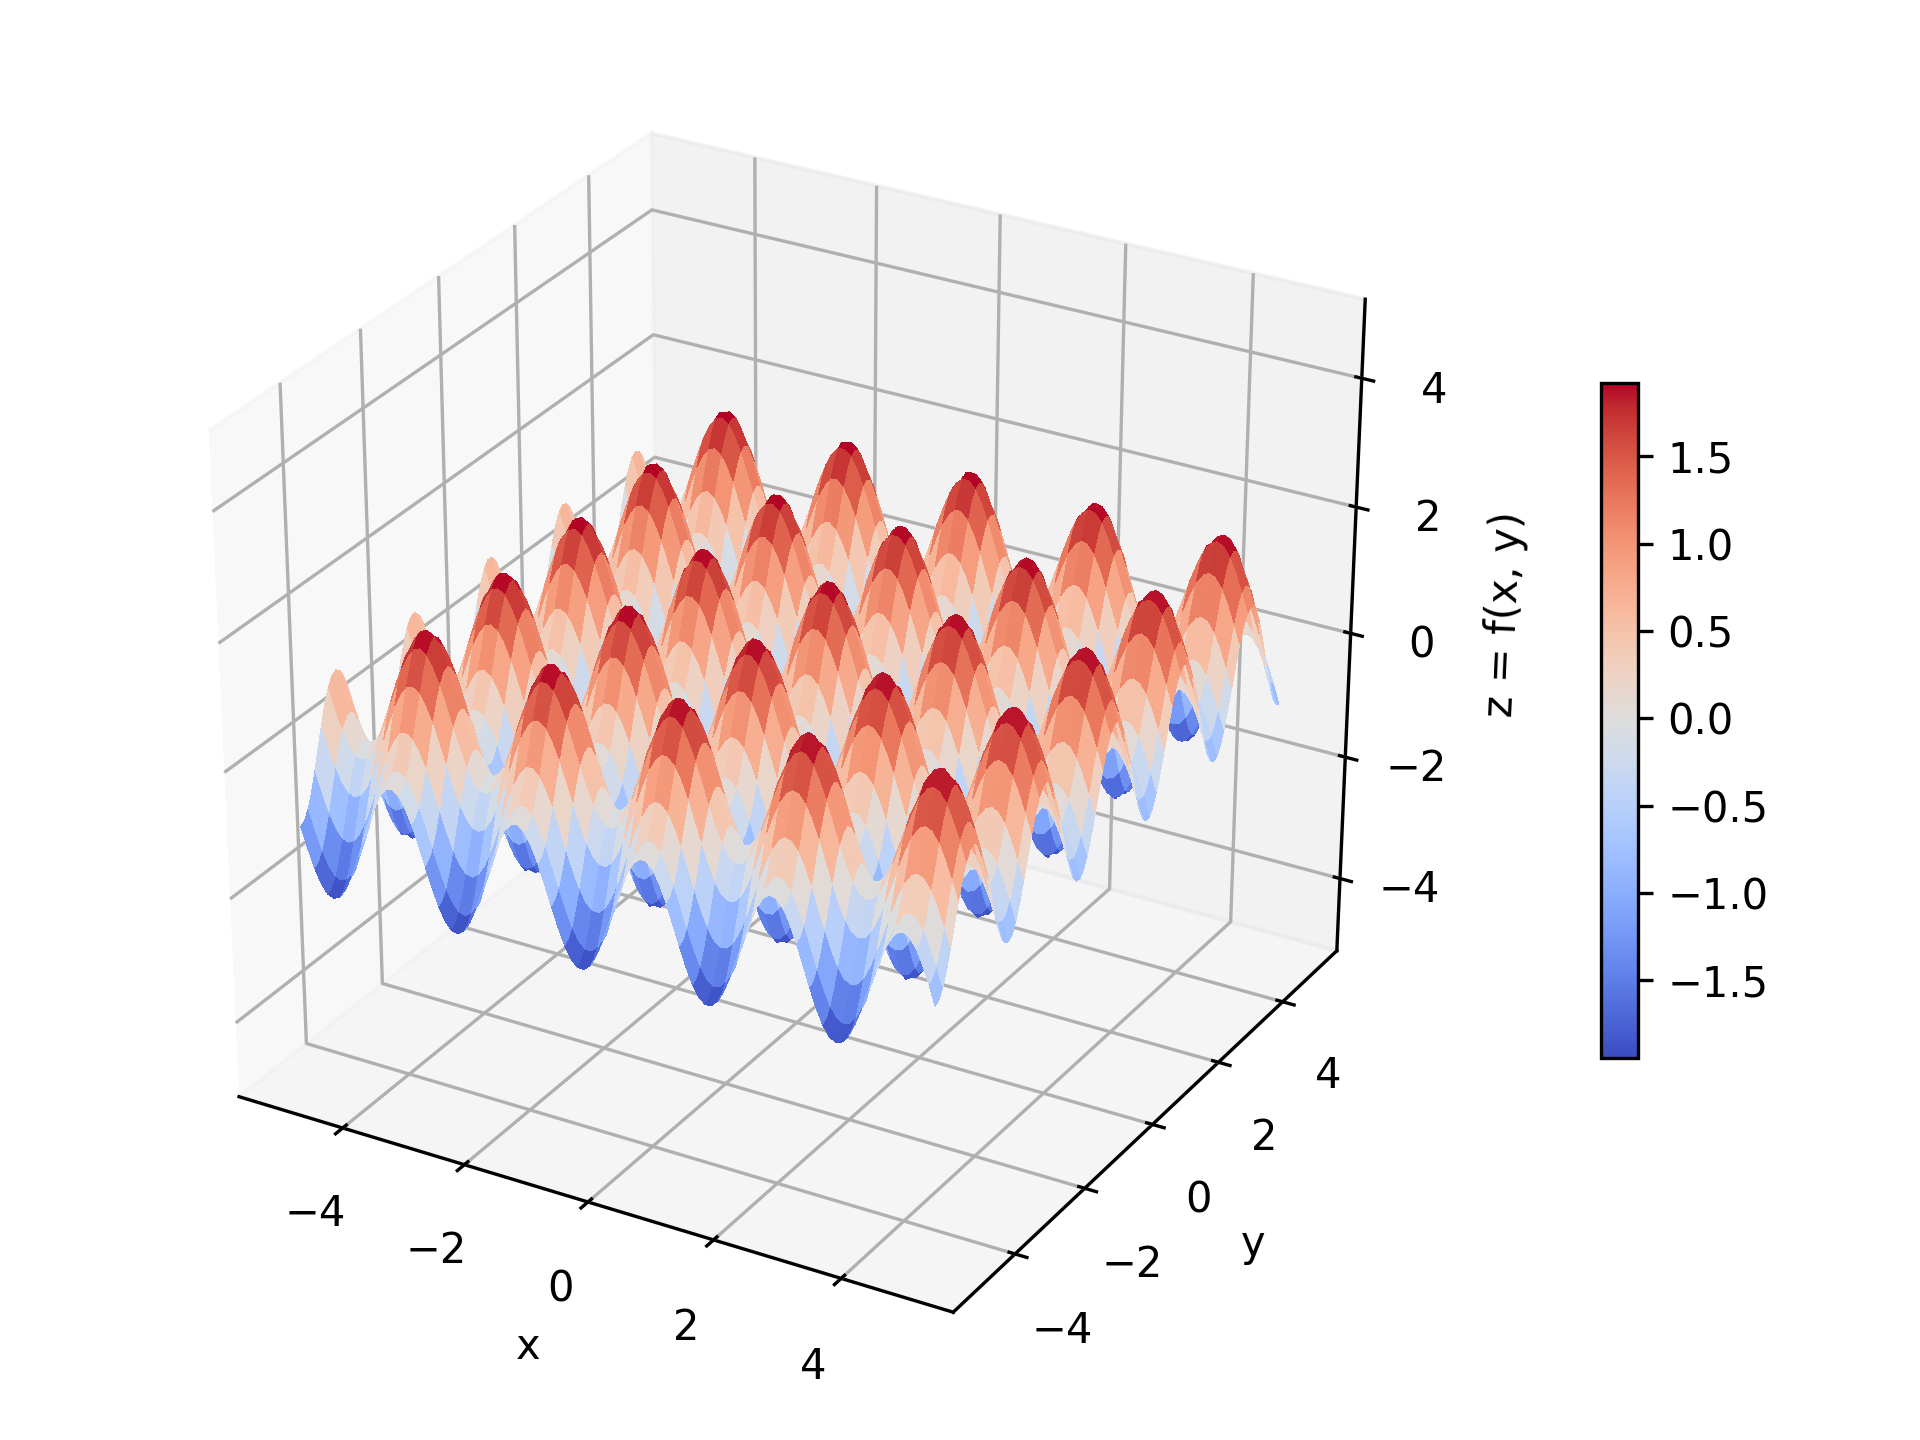
\includegraphics[width=.8\linewidth]{functions/sinx+cosy.png}
    \caption{two-dimensional periodic function ($f_4$)}
  \end{subfigure}
  \caption{Functions sampled for our datasets.}
  \label{fig:1}
\end{figure}

\subsection{Sampling procedure}

For each one-dimensional function ($f_1, f_2, f_3$), we created sample size of 5, 10 and 50 data points, ranging from -5 to 5 in the independent variable. We applied this sampling procedure for training and test sets.

\subsection{Kernel parameters}

In our model, the default kernel function will be the squared-exponential (SE) kernel. For instance, the one-dimensional case is given by Eq.\eqref{eq:kernelSE}, where $\alpha = (\sigma, \ell)$ is the vector of hyperparameters. In addition, we have the prior of the noise's standard deviation ($\sigma_y^2$), which also has effect on our predictions. The default value of $\sigma$, $\ell$ and $\sigma_y^2$ are 1, 1 and 0.1, respectively.

\begin{equation}\
  \label{eq:kernelSE}
  \kappa_{SE}(x,x') = \sigma^2 \exp{\left(-\dfrac{(x-x')^2}{2\ell^2}\right)}
\end{equation} 

Hence, we will evaluate the effects of different hyperparameters ($\sigma$, $\ell$ and $\sigma_y^2$) on the predictions of our regression. We applied the following values of $\sigma$: 0.01, 0.1, 0.5, 1, 10 and 100; the following values of $\ell$: 0.1, 1, 2, 5, 10 and 100; and the following values of $\sigma_y^2$: 0.001, 0.01, 0.1, 1, 2 and 10.

\subsection{Kernel functions}

As mentioned above, we chose the SE kernel as our default basis function; however, we can choose different kernel functions. Then, we choose Ornstein-Uhlenbeck (OU; Eq.\eqref{eq:kernelOU}), Rational Quadratic (RQ; Eq.\eqref{eq:kernelRQ}) and Exponential Sine Squared (ESS; Eq.\eqref{eq:kernelESS}) kernels to evaluate the effect of the kernel function on predictions.

\begin{equation}
  \label{eq:kernelOU}
  \kappa_{OU}(x,x') = \sigma^2 \exp{\left(-\frac{|x-x'|}{2\ell^2}\right)}  
\end{equation}

\begin{equation}
  \label{eq:kernelRQ}
  \kappa_{RQ}(x,x') = \sigma^2 \left(1 + \frac{(x-x')^2}{2\alpha\ell^2}\right)^{-\alpha}
\end{equation}

\begin{equation}
  \label{eq:kernelESS}
  \kappa_{ESS}(x,x') = \sigma^2 \exp{\left(-\frac{2\sin\left(\frac{\pi|x-x'|}{w}\right)^2}{\ell^2}\right)}
\end{equation}

\subsection{Higher dimensional data}

Until now, our model are handling one-dimensional data, in order to calculate higher dimensional data, we need to extend the SE kernel from Eq.\eqref{eq:kernelSE} to multidimensional data as follows:

\begin{equation}
  \kappa(x_p,x_q) = \sigma^2_f\exp{\left(-\frac{1}{2}(x_p - x_q)^TM(x_p - x_q)\right)}
  \label{eq:multi}
\end{equation}
where the matrix $M$ can be defined in several ways, but we use an isotropic matrix $M = \ell^{-2}I$.

\section{Results}

\subsection{Effect of Sample Size}

Here, we evaluate the different samples sizes for the training and test sets. 

\subsubsection{Training set}
We evaluated effects of the training set size on our predictions, keeping the test set size fixed in 50 samples (Fig \ref{fig:train_samples}). In the plot, the blue dashed curve represented our target, the red line is our prediction of the target, and the light red region represents our confidence interval (level of uncertainty about the predicted value of our fitted function). We observed that regions where we had observations has less uncertainty in our prediction, \ie a smaller confidence interval. On the other hand, regions with no observation has a higher uncertainty, \ie a wider confidence interval. In addition, the distance bewteen two observations determine the uncertainty in the region between them; hence, smaller the distance, lower are the uncertainty. Further, with the increase of the training set size, our predictions gets relatively close to the target function. Therefore, we observed that 50 samples are a sufficient amount of training points to obtain a reliable curve in the studied range.

\begin{figure}
\begin{subfigure}{.33\textwidth}
  \centering
  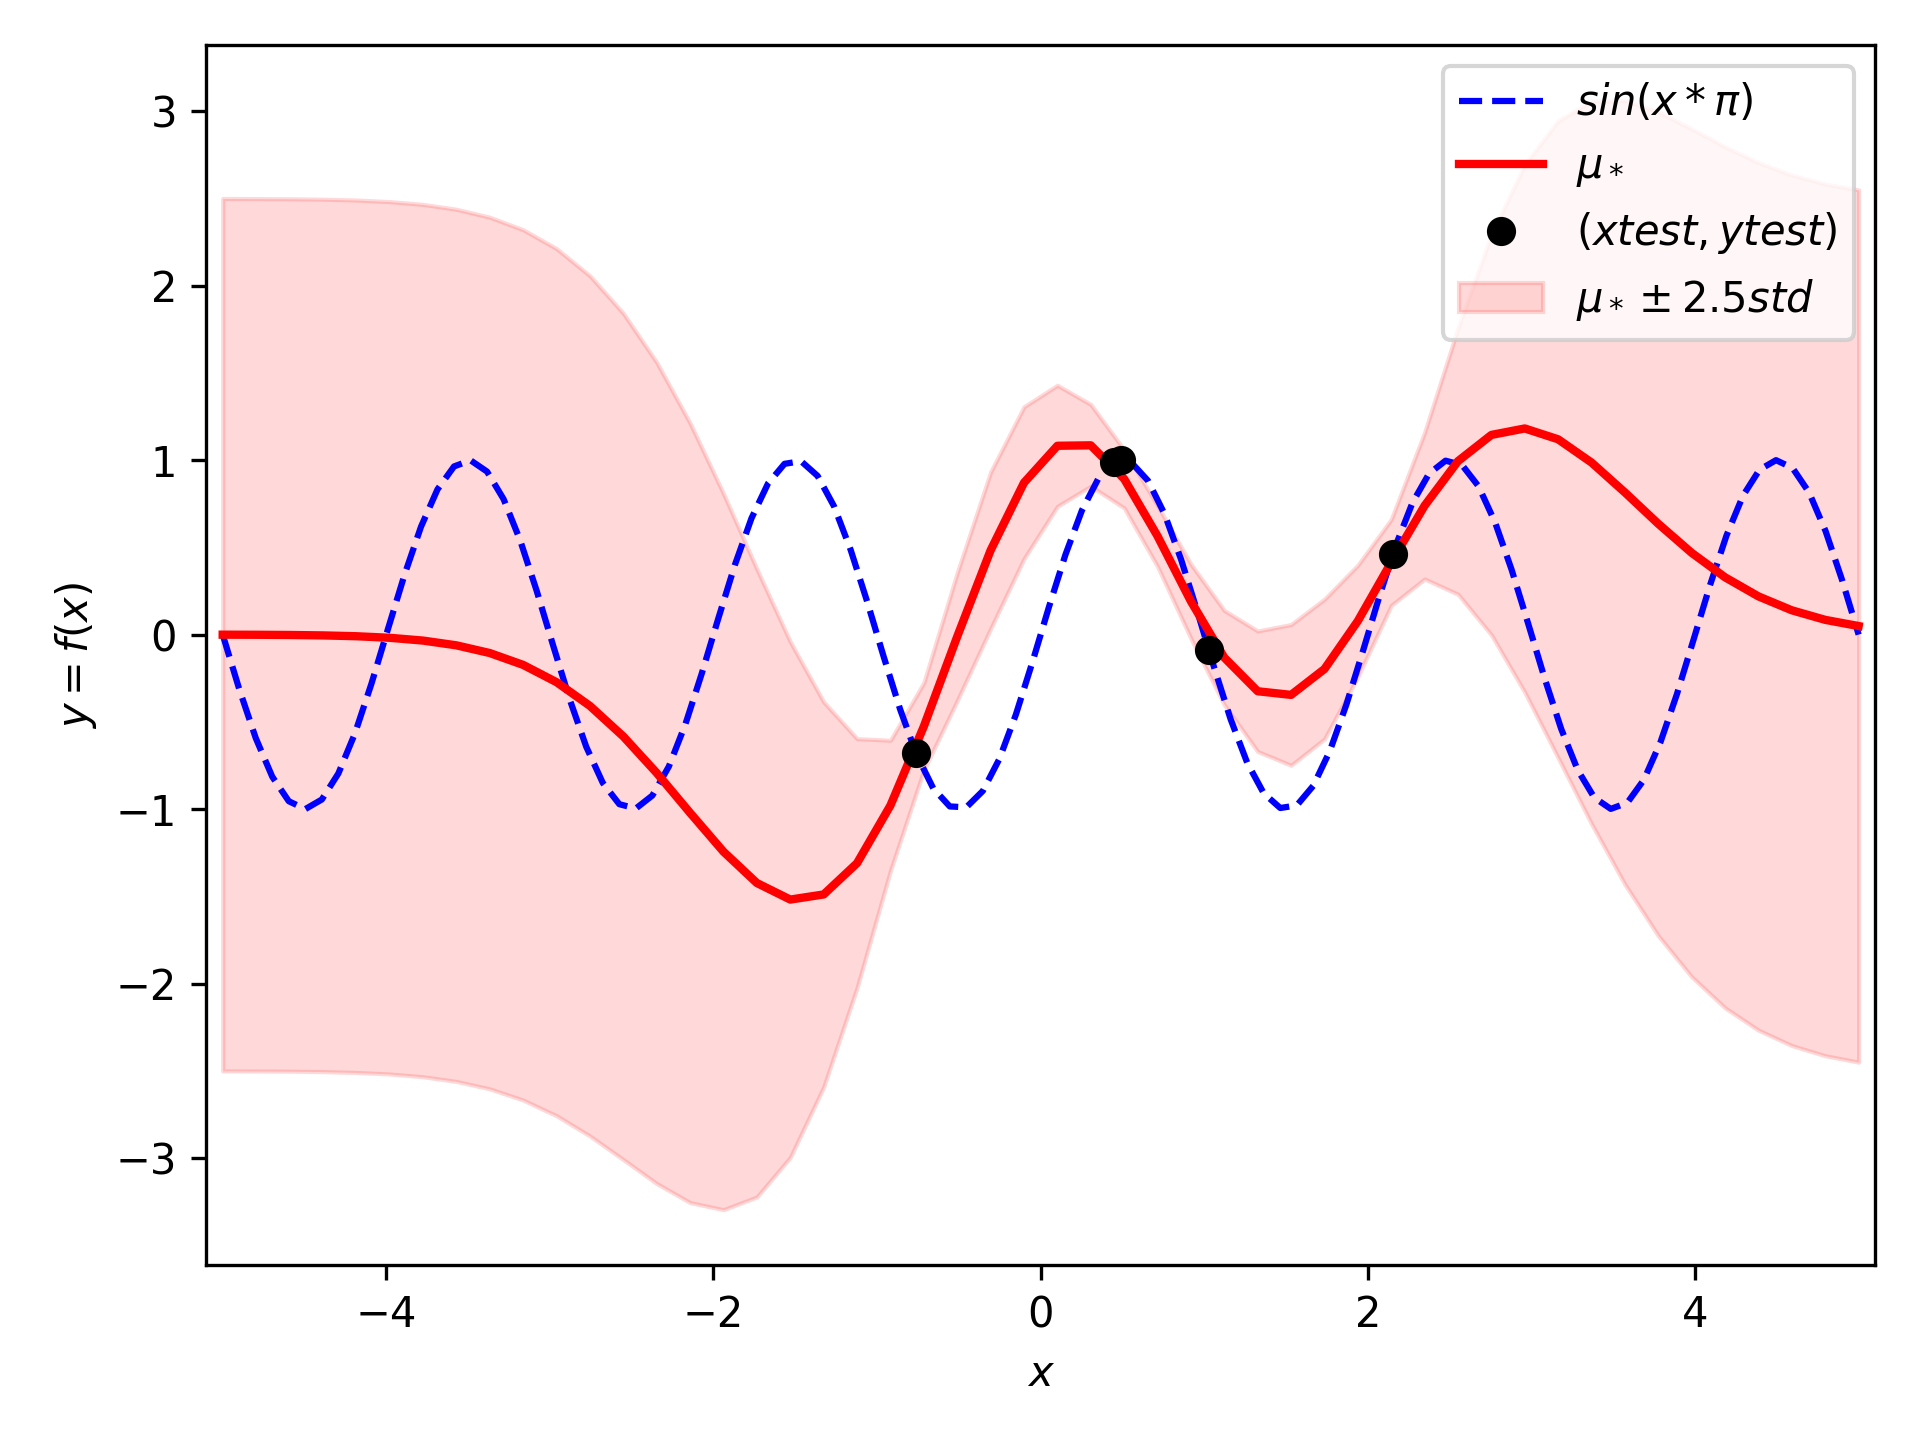
\includegraphics[width=\linewidth]{train_size/func1_5.png}
  \caption{$f_1; S = 5$}
\end{subfigure}
\begin{subfigure}{.33\textwidth}
  \centering
  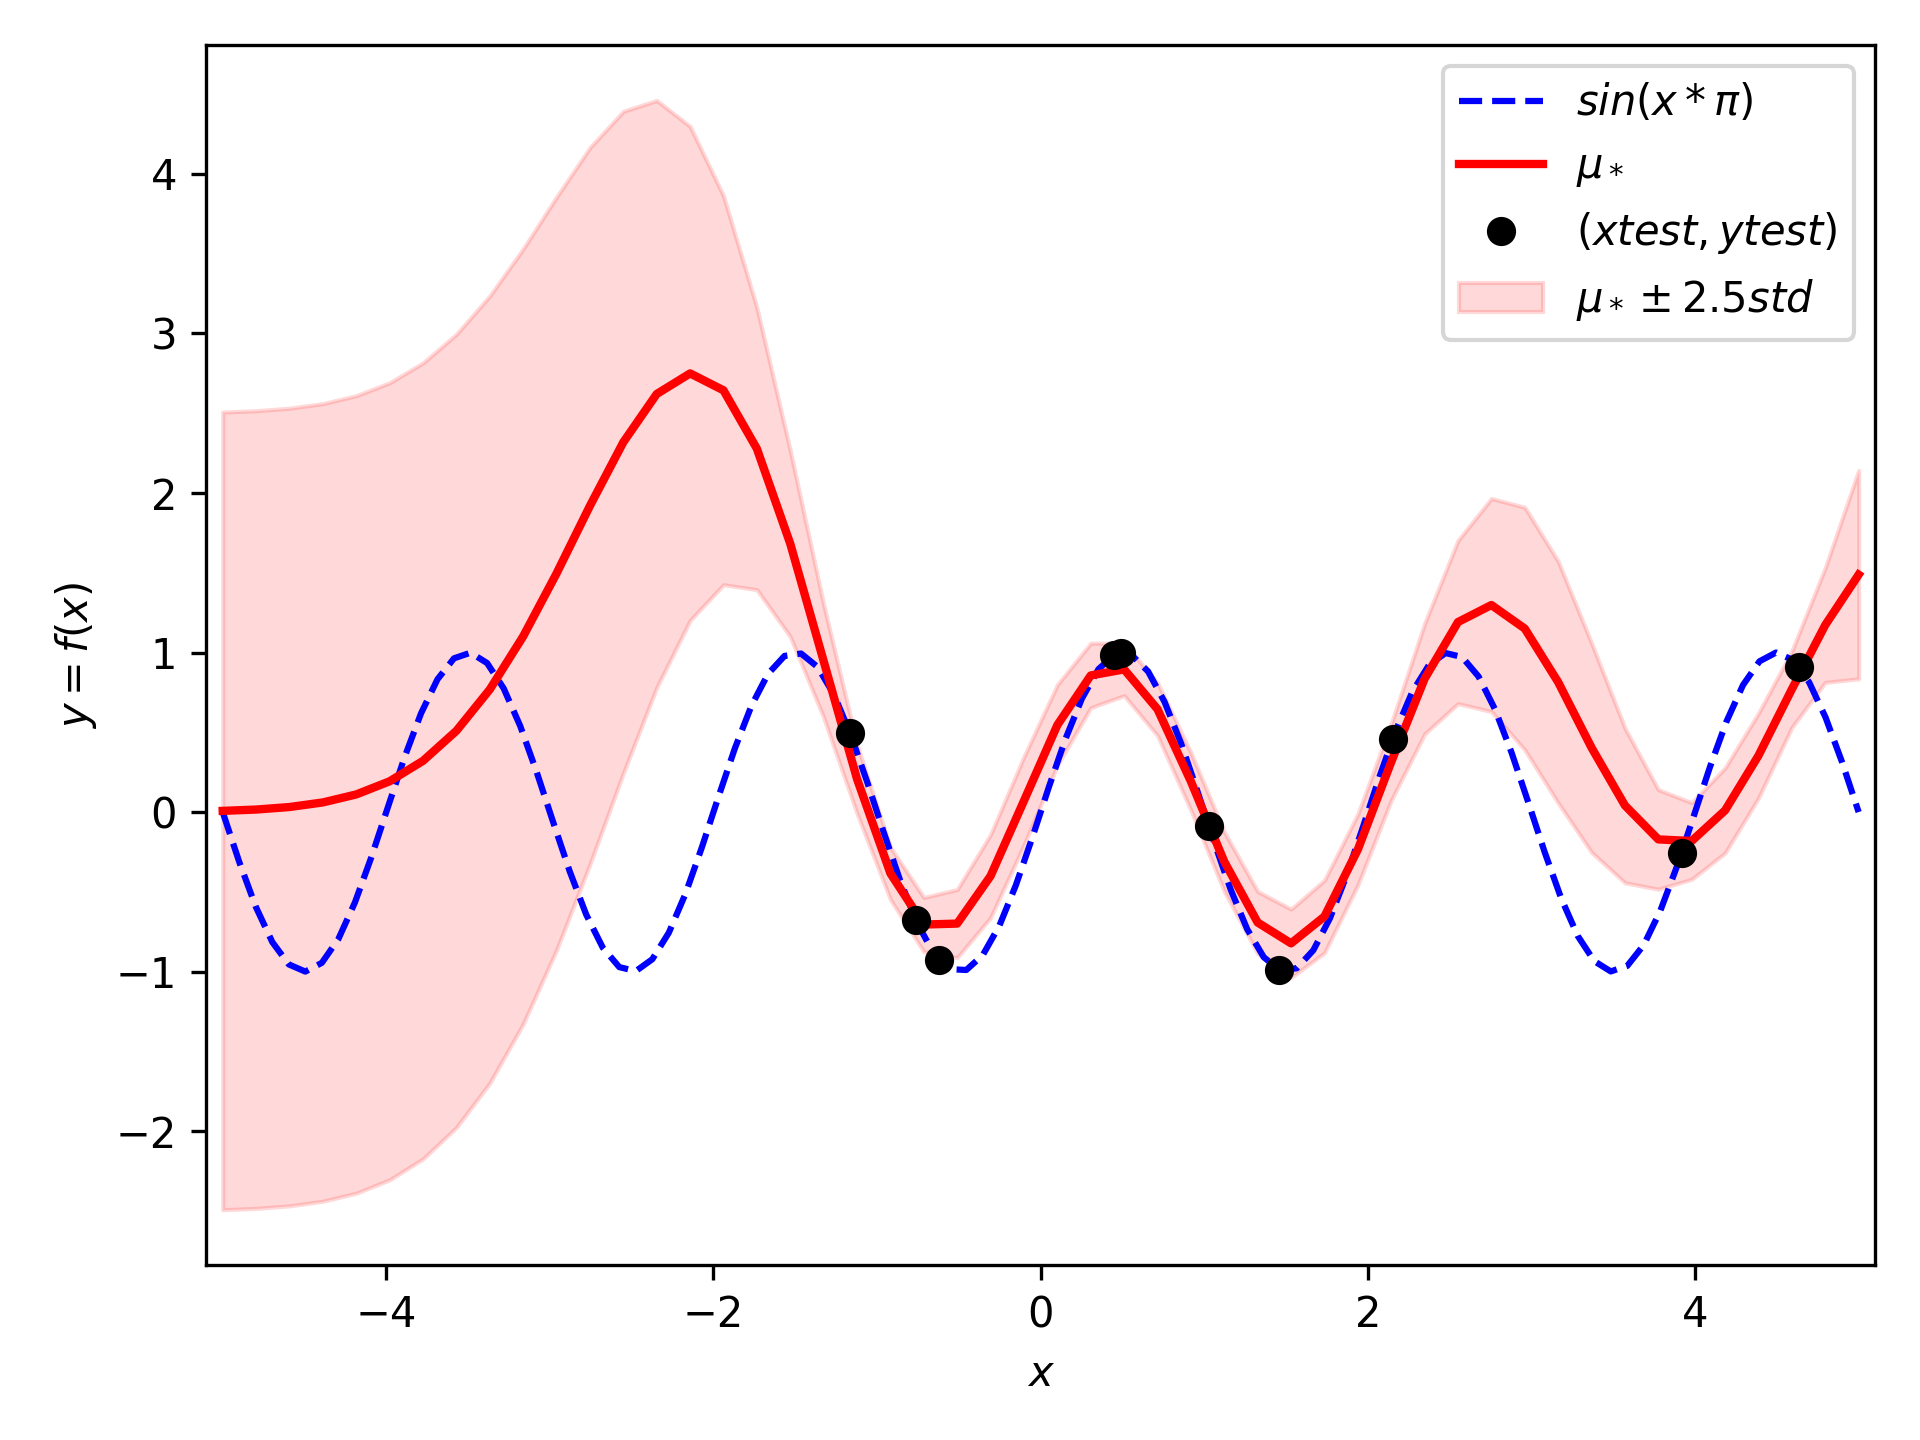
\includegraphics[width=\linewidth]{train_size/func1_10.png}
  \caption{$f_1; S = 10$}
\end{subfigure}
\begin{subfigure}{.33\textwidth}
  \centering
  \includegraphics[width=\linewidth]{train_size/func1_50.png}
  \caption{$f_1; S = 50$}
\end{subfigure}
\begin{subfigure}{.33\textwidth}
  \centering
  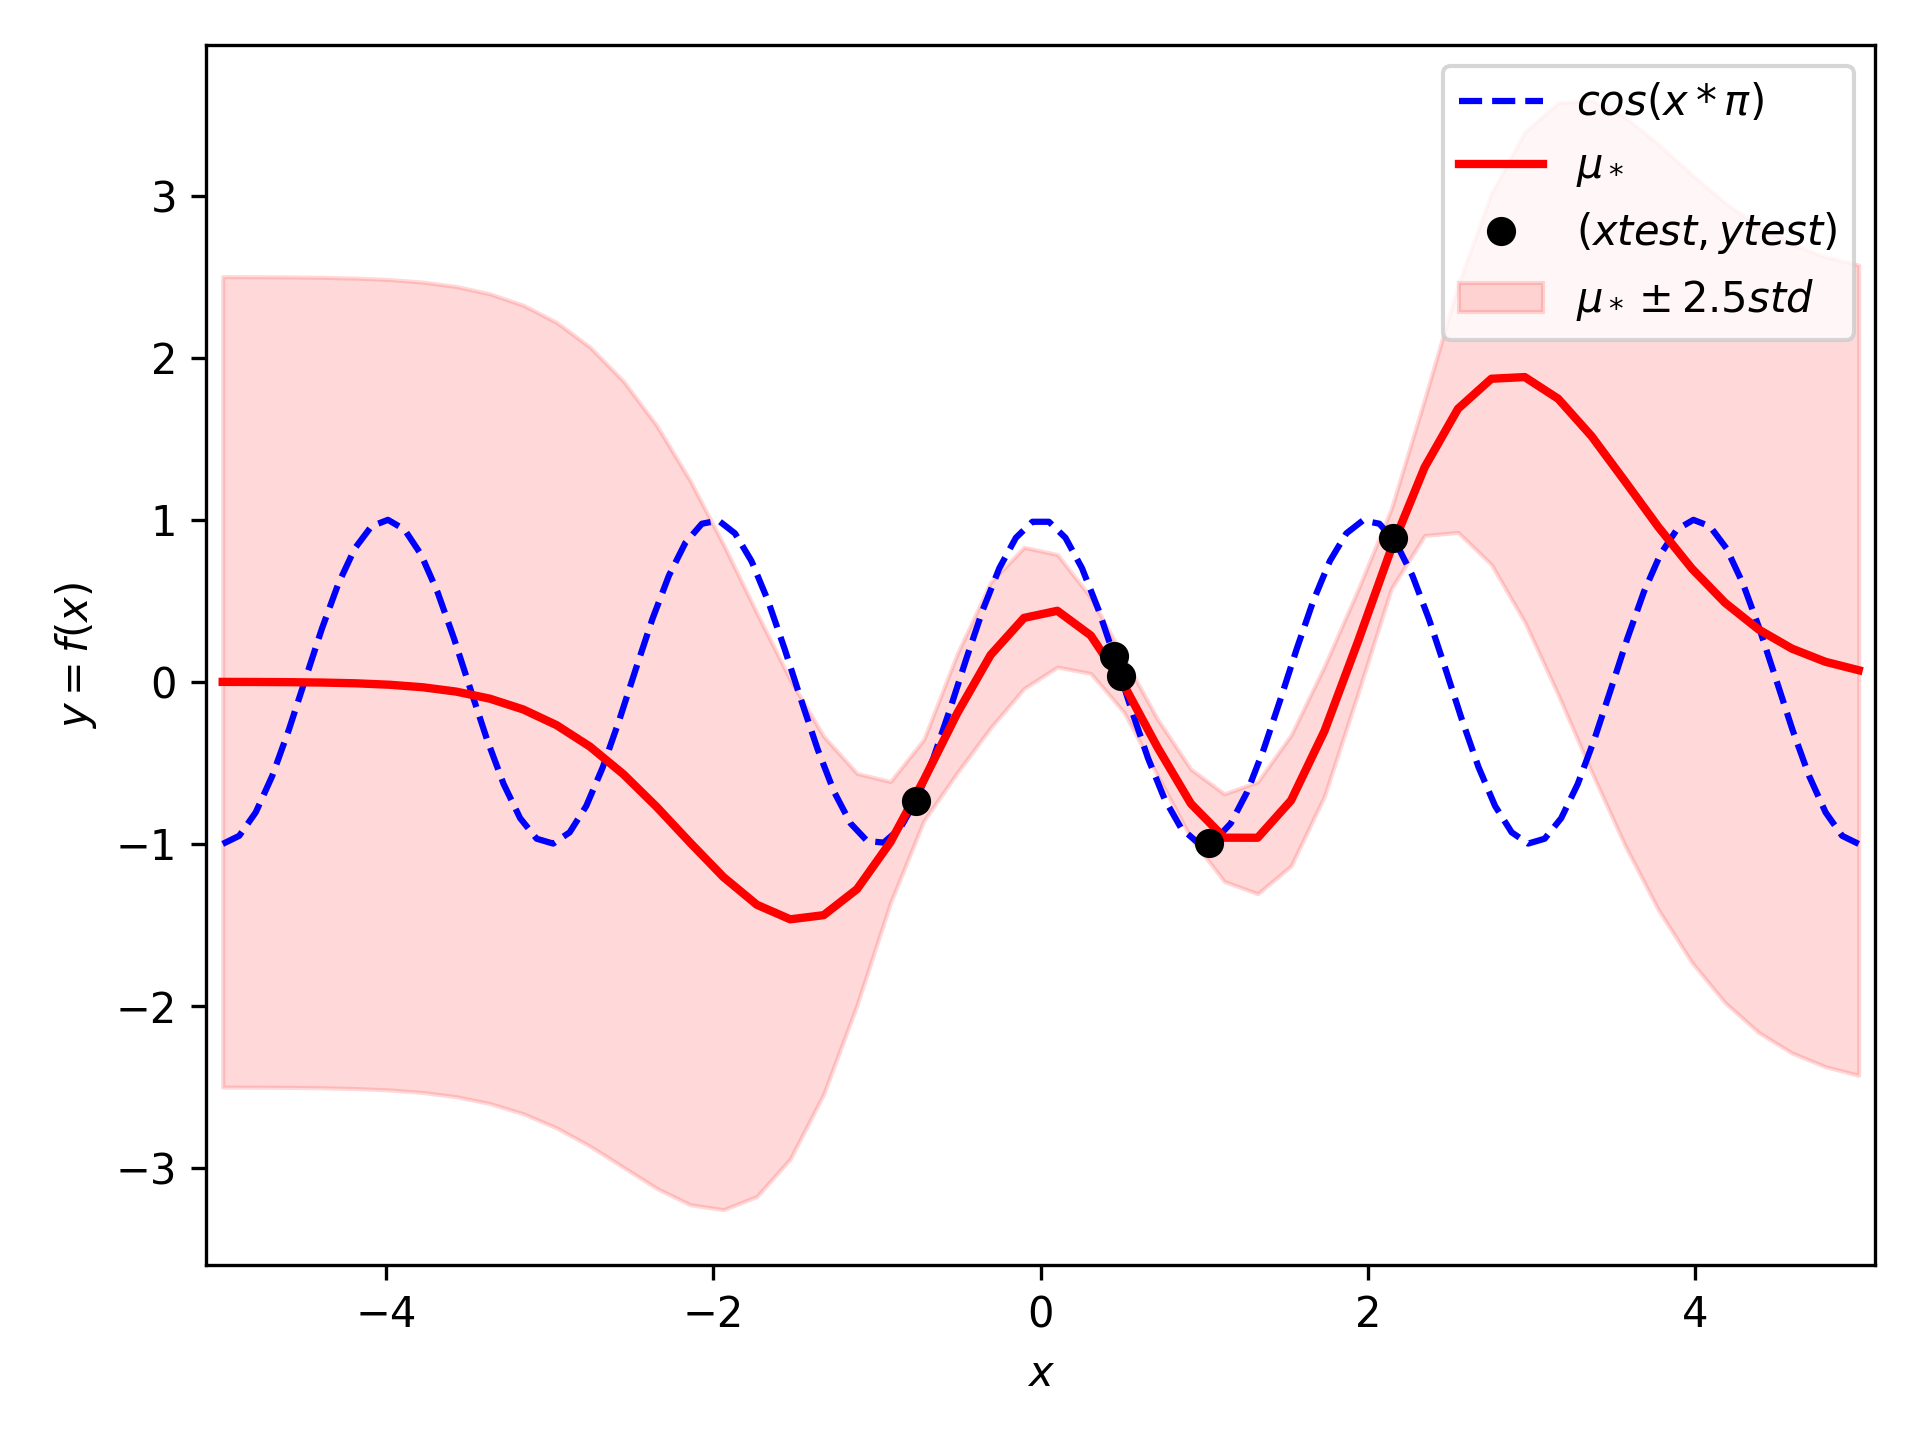
\includegraphics[width=\linewidth]{train_size/func2_5.png}
  \caption{$f_2; S = 5$}
\end{subfigure}
\begin{subfigure}{.33\textwidth}
  \centering
  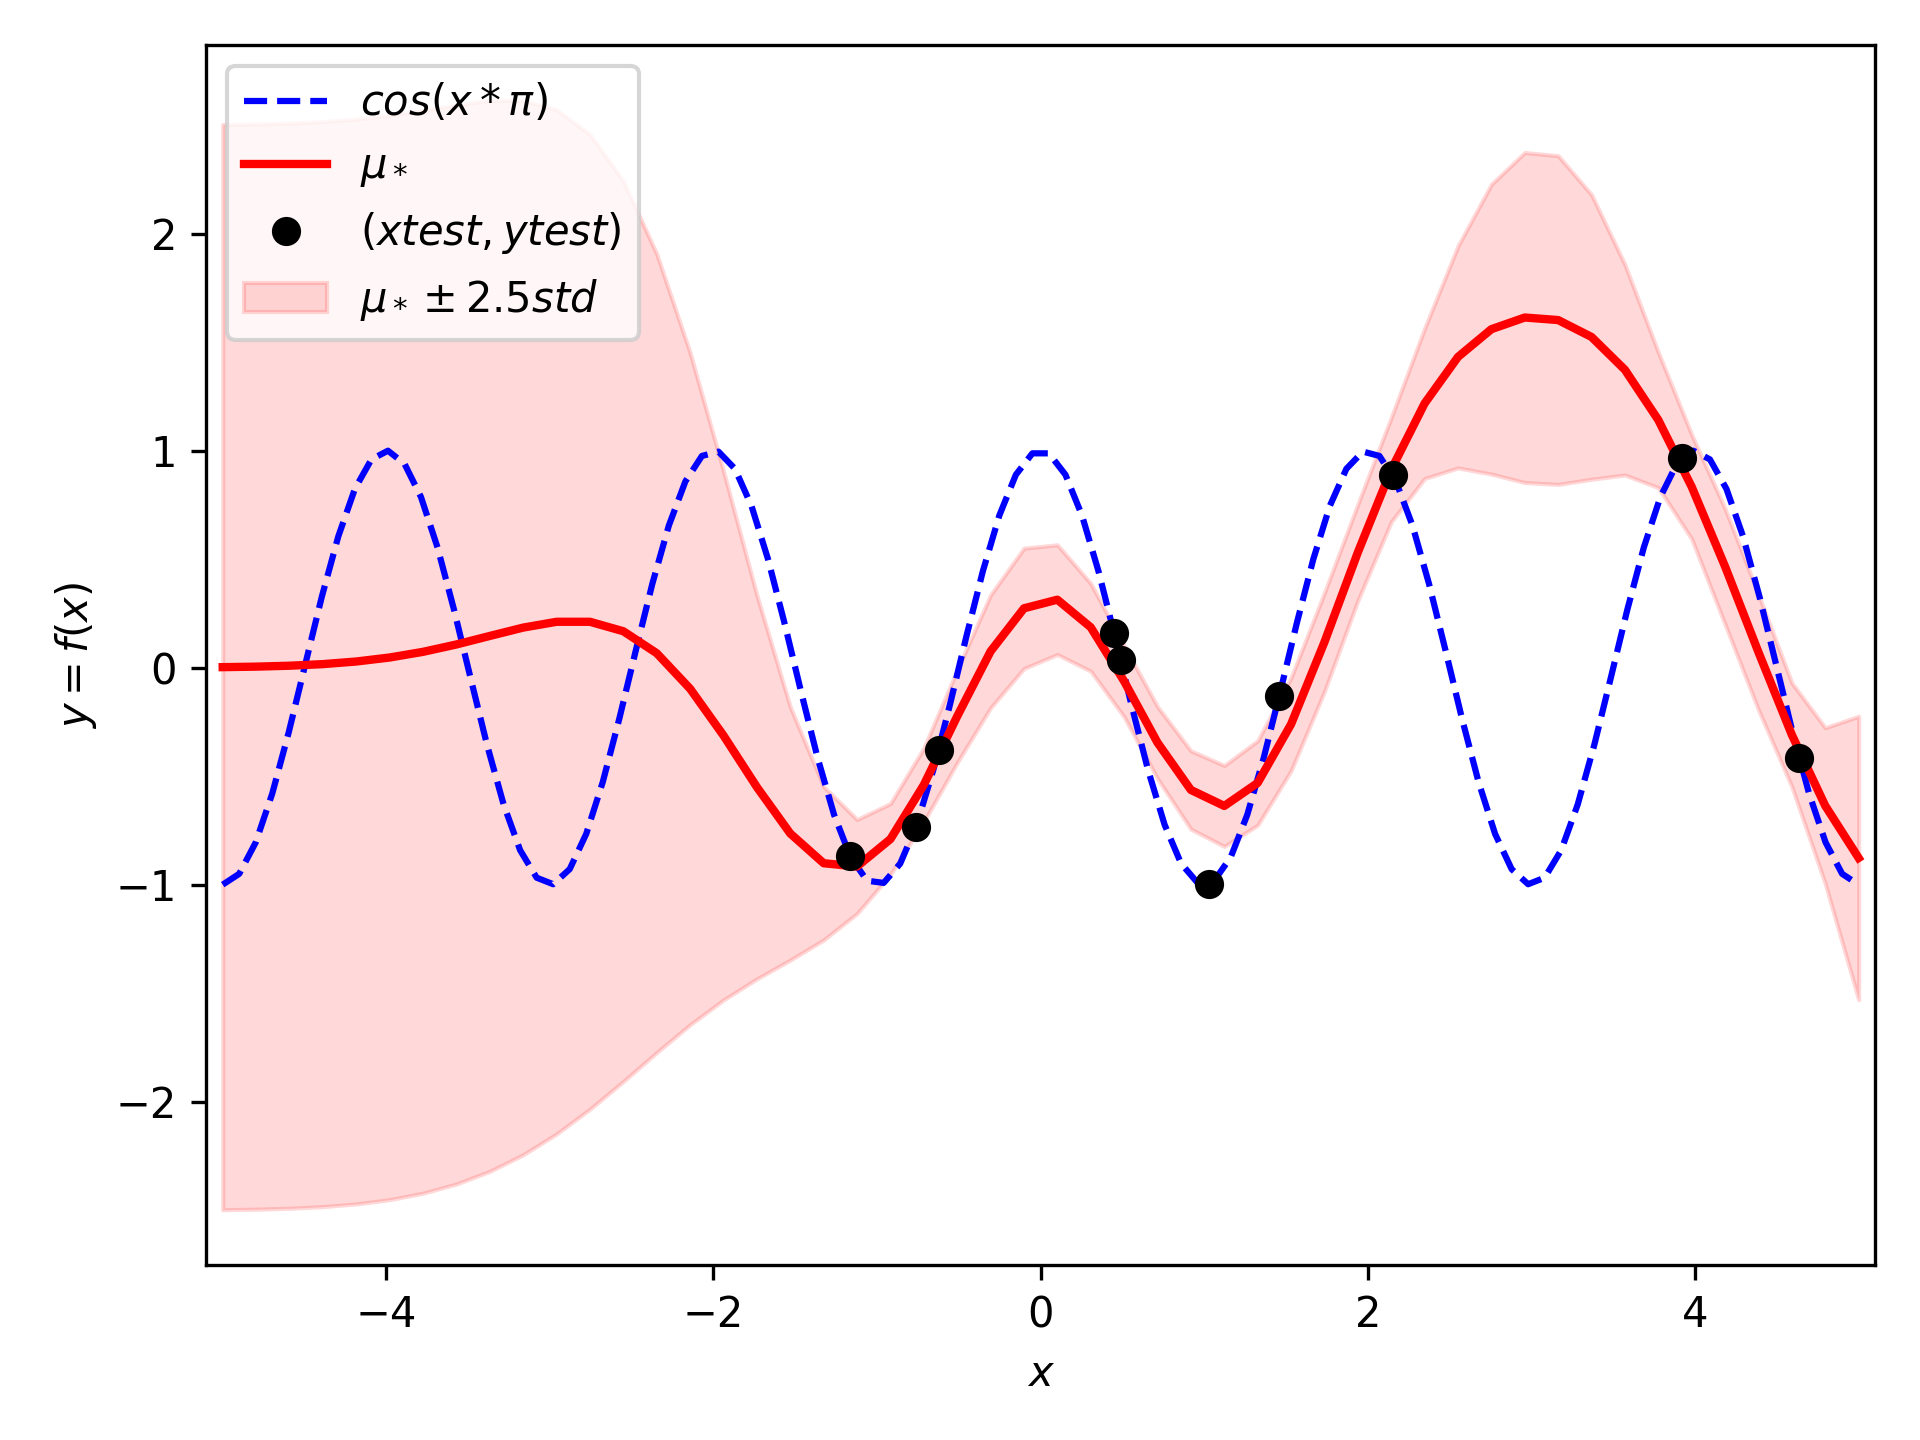
\includegraphics[width=\linewidth]{train_size/func2_10.png}
  \caption{$f_2; S = 10$}
\end{subfigure}
\begin{subfigure}{.33\textwidth}
  \centering
  \includegraphics[width=\linewidth]{train_size/func2_50.png}
  \caption{$f_2; S = 50$}
\end{subfigure}
\begin{subfigure}{.33\textwidth}
  \centering
  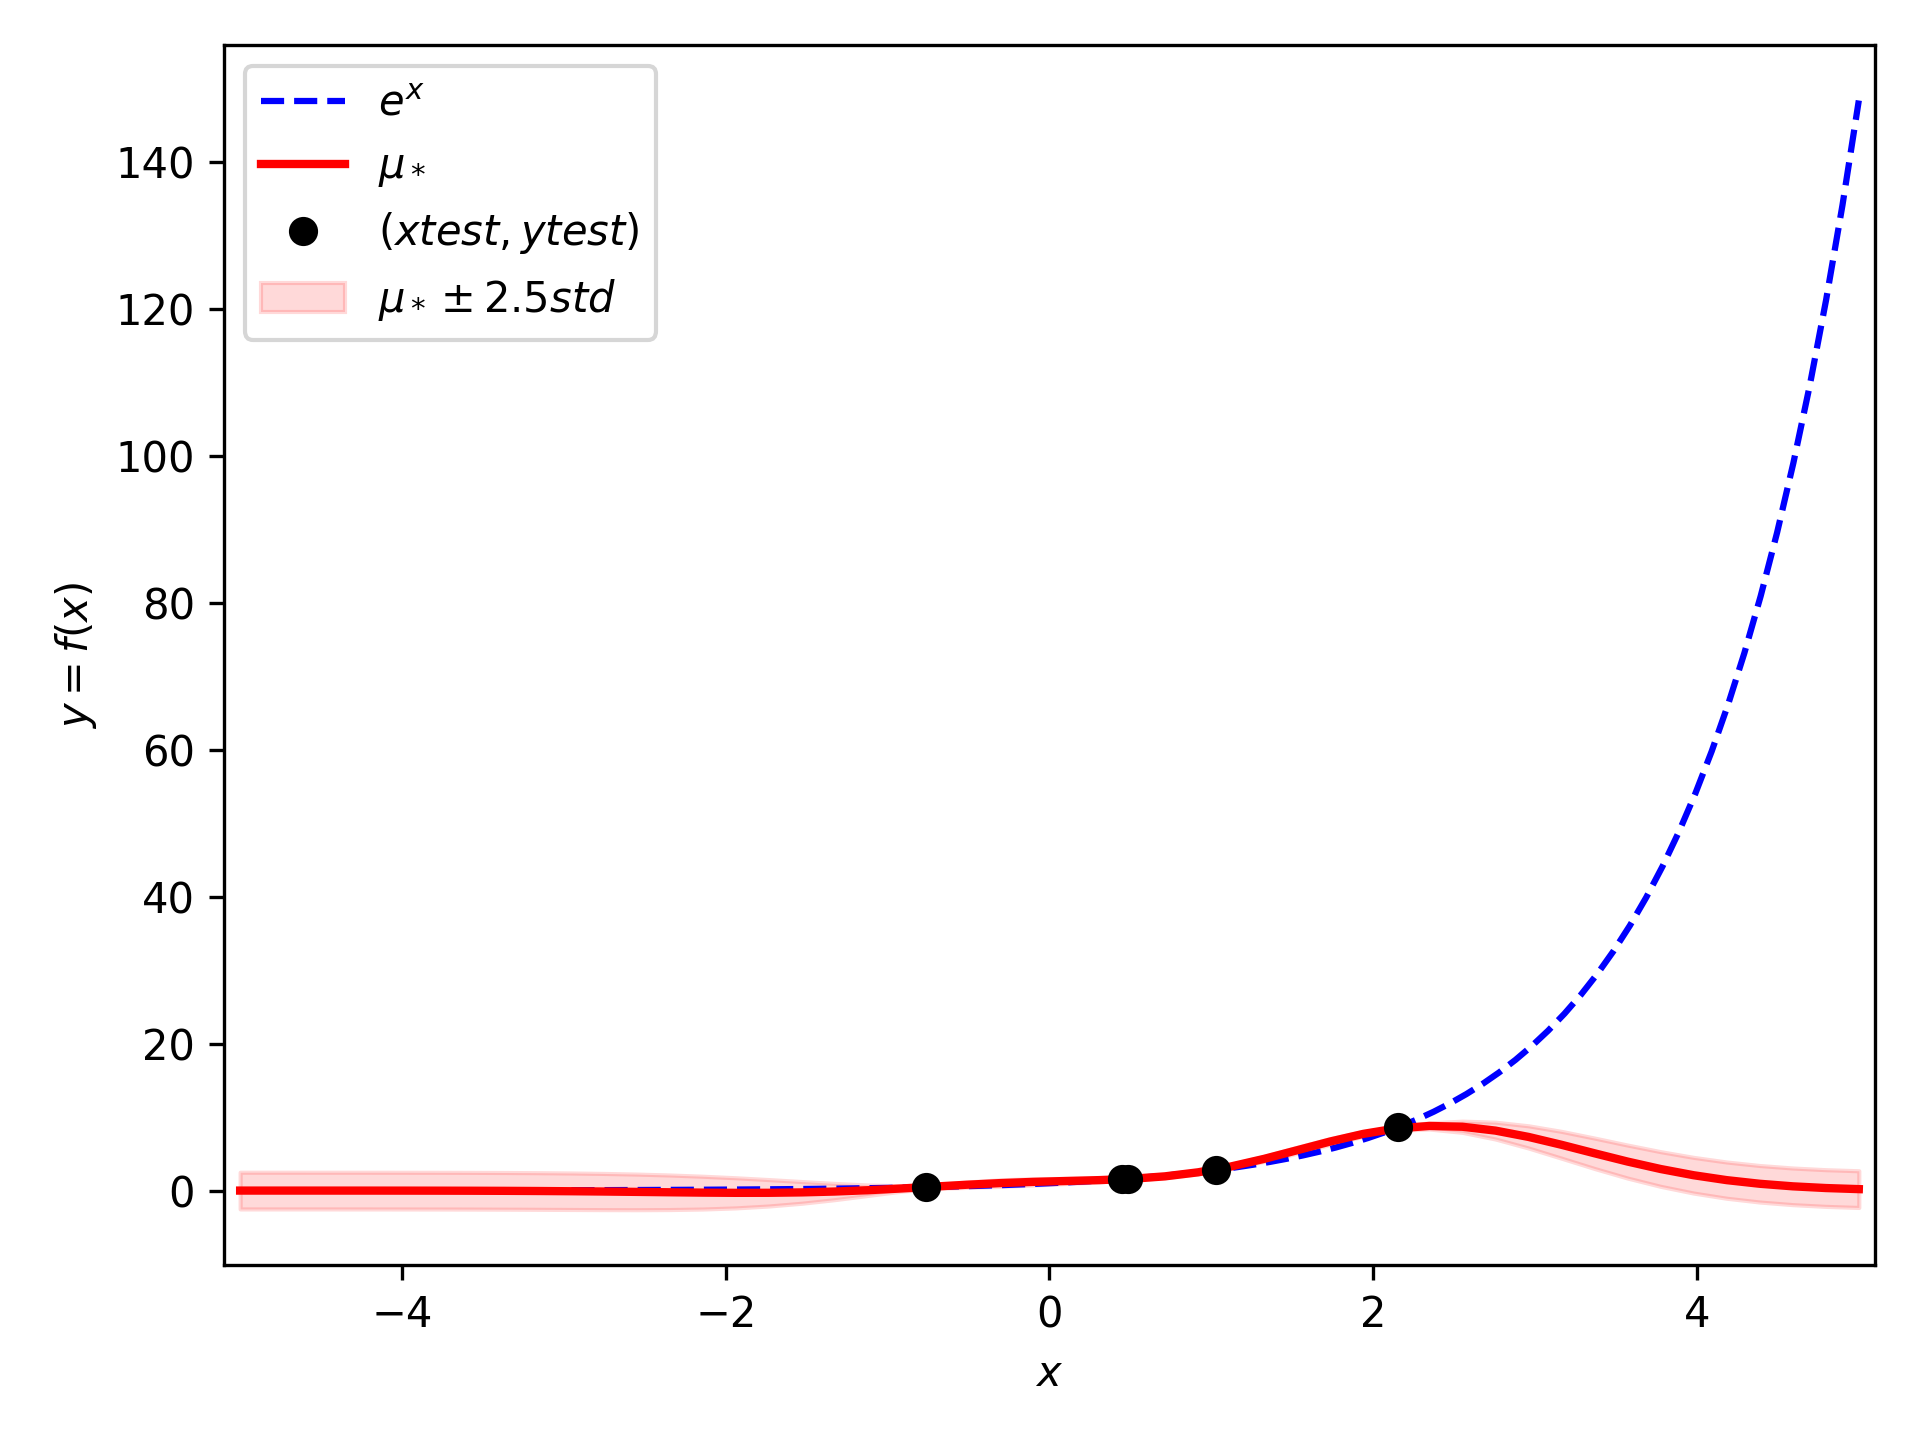
\includegraphics[width=\linewidth]{train_size/func3_5.png}
  \caption{$f_3; S = 5$}
\end{subfigure}
\begin{subfigure}{.33\textwidth}
  \centering
  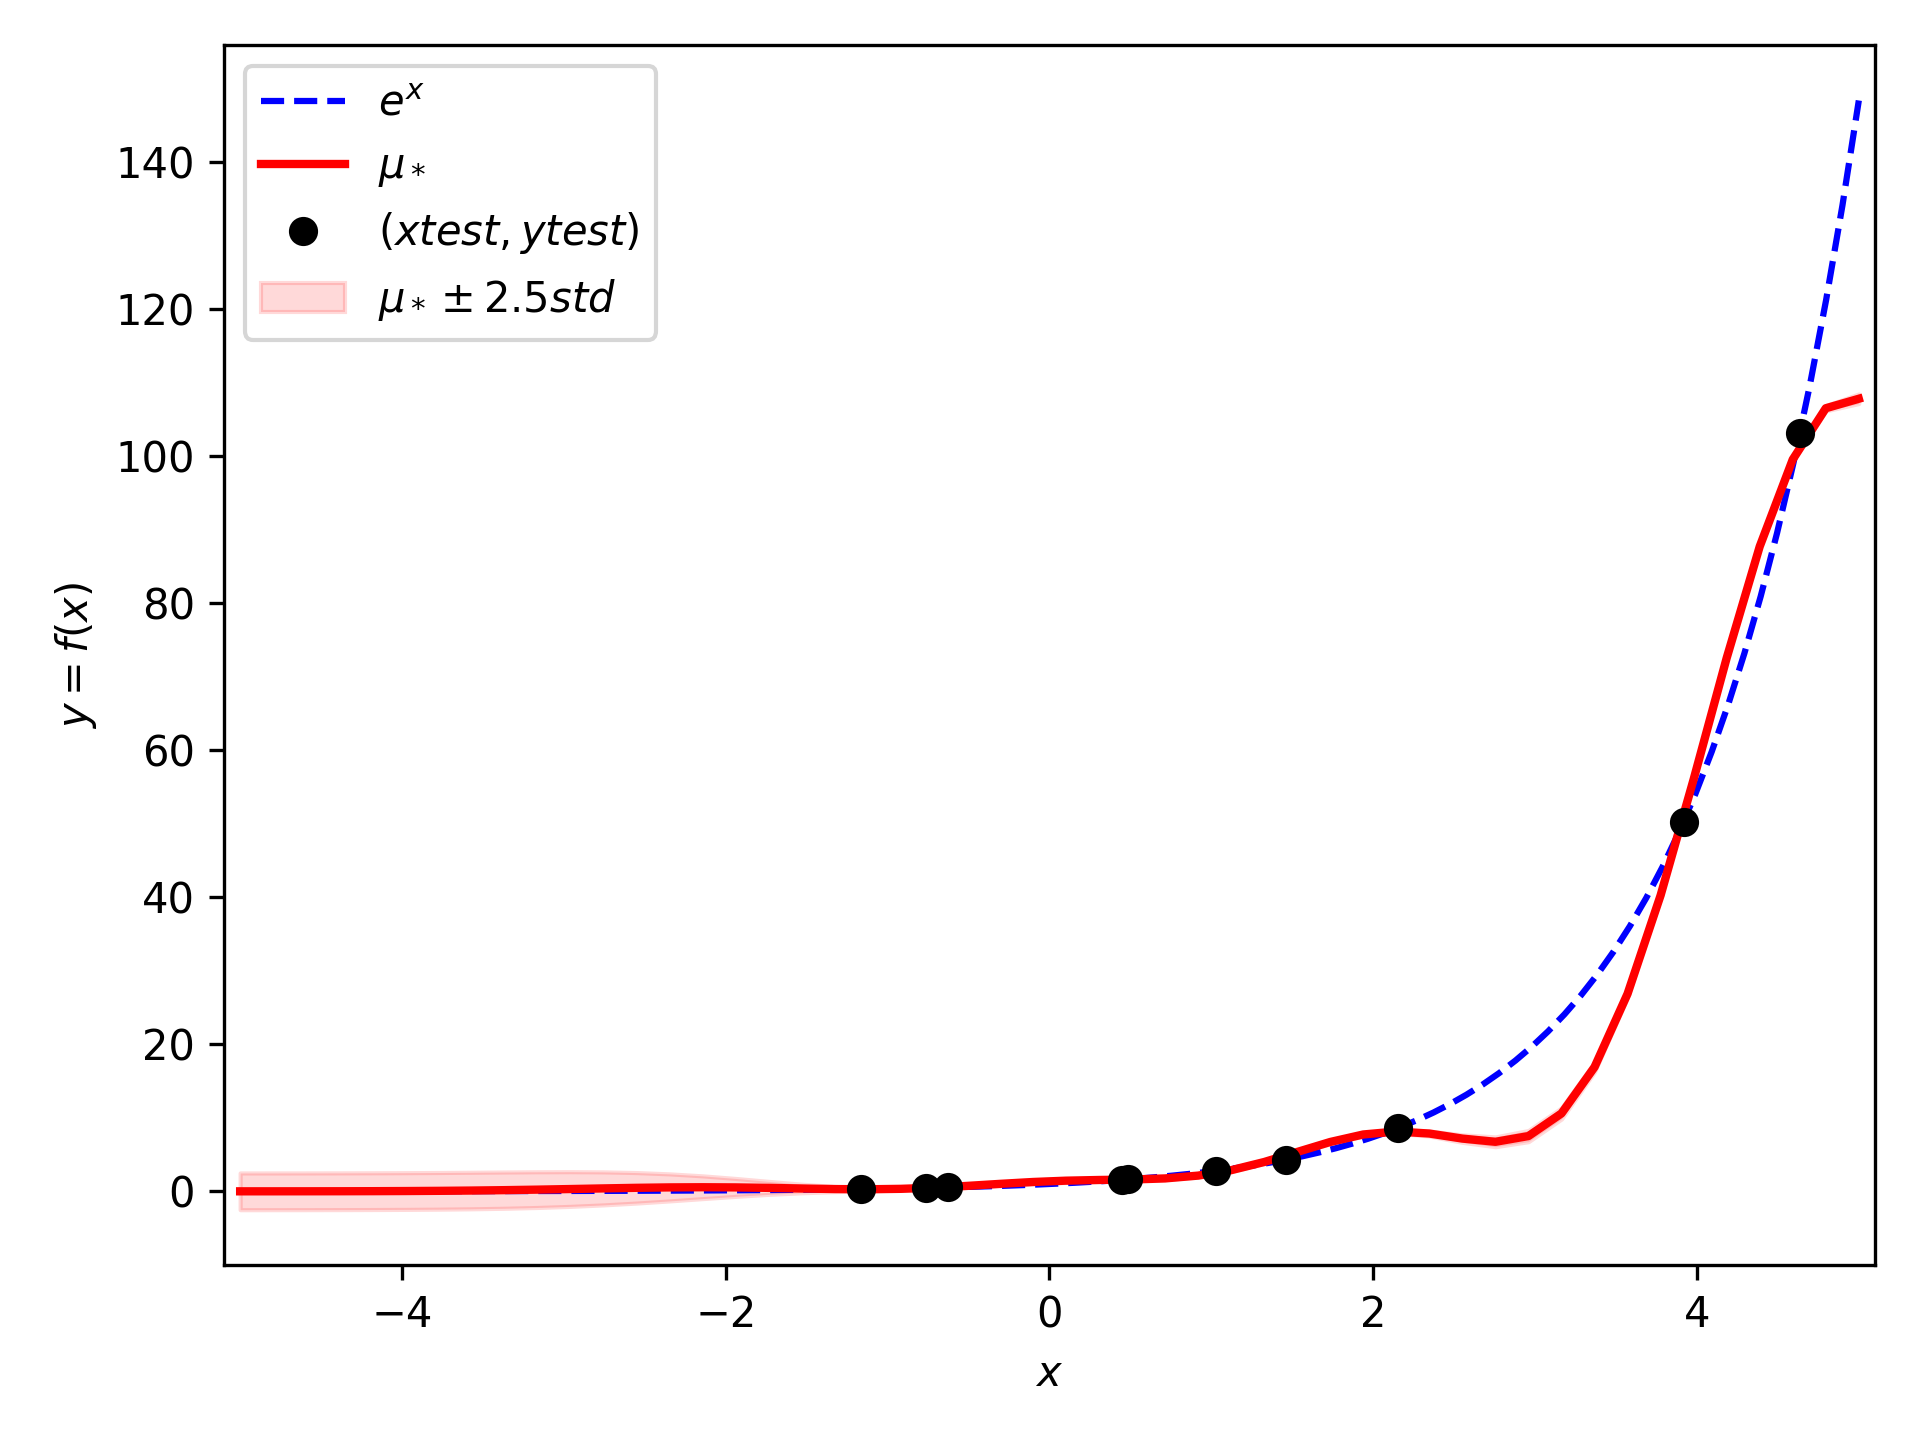
\includegraphics[width=\linewidth]{train_size/func3_10.png}
  \caption{$f_3; S = 10$}
\end{subfigure}
\begin{subfigure}{.33\textwidth}
  \centering
  \includegraphics[width=\linewidth]{train_size/func3_50.png}
  \caption{$f_3; S = 50$}
\end{subfigure}
\caption{Gaussian Processes with SE kernel with different training set sizes (S). The samples comes from three different functions (sine - $f_1$, cosine - $f_2$ and exponential - $f_3$).}
\label{fig:train_samples}
\end{figure}

\subsubsection{Test set}

We evaluated effects of the test set size on our predictions, keeping the training set size fixed in 50 samples (Fig \ref{fig:test_samples}). We observed that with more points in the test set, the uncertainty decreases in our prediction, \ie a smaller confidence interval; however, this effect is lesser when compared to the effect of varying the training set size. In addition, a small number of samples in the test set yields an incorrect prediction of our target, as can be seen for 5 samples, almost being possible to define which points where used in the test set. Then, with the increasing number of samples in the test set, our predictions gets relatively close to the target function. Finally, we suggest that the model appears to use the test samples to interpolate the fitted curve based on the training set information.

Therefore, we observed that 50 samples are a sufficient amount of test points to obtain a reliable curve in the studied range. However, the exponential curve had already achieved a reliable prediction with 10 samples, showing that there are no universal sample size for our model. 

\begin{figure}
  \begin{subfigure}{.33\textwidth}
    \centering
    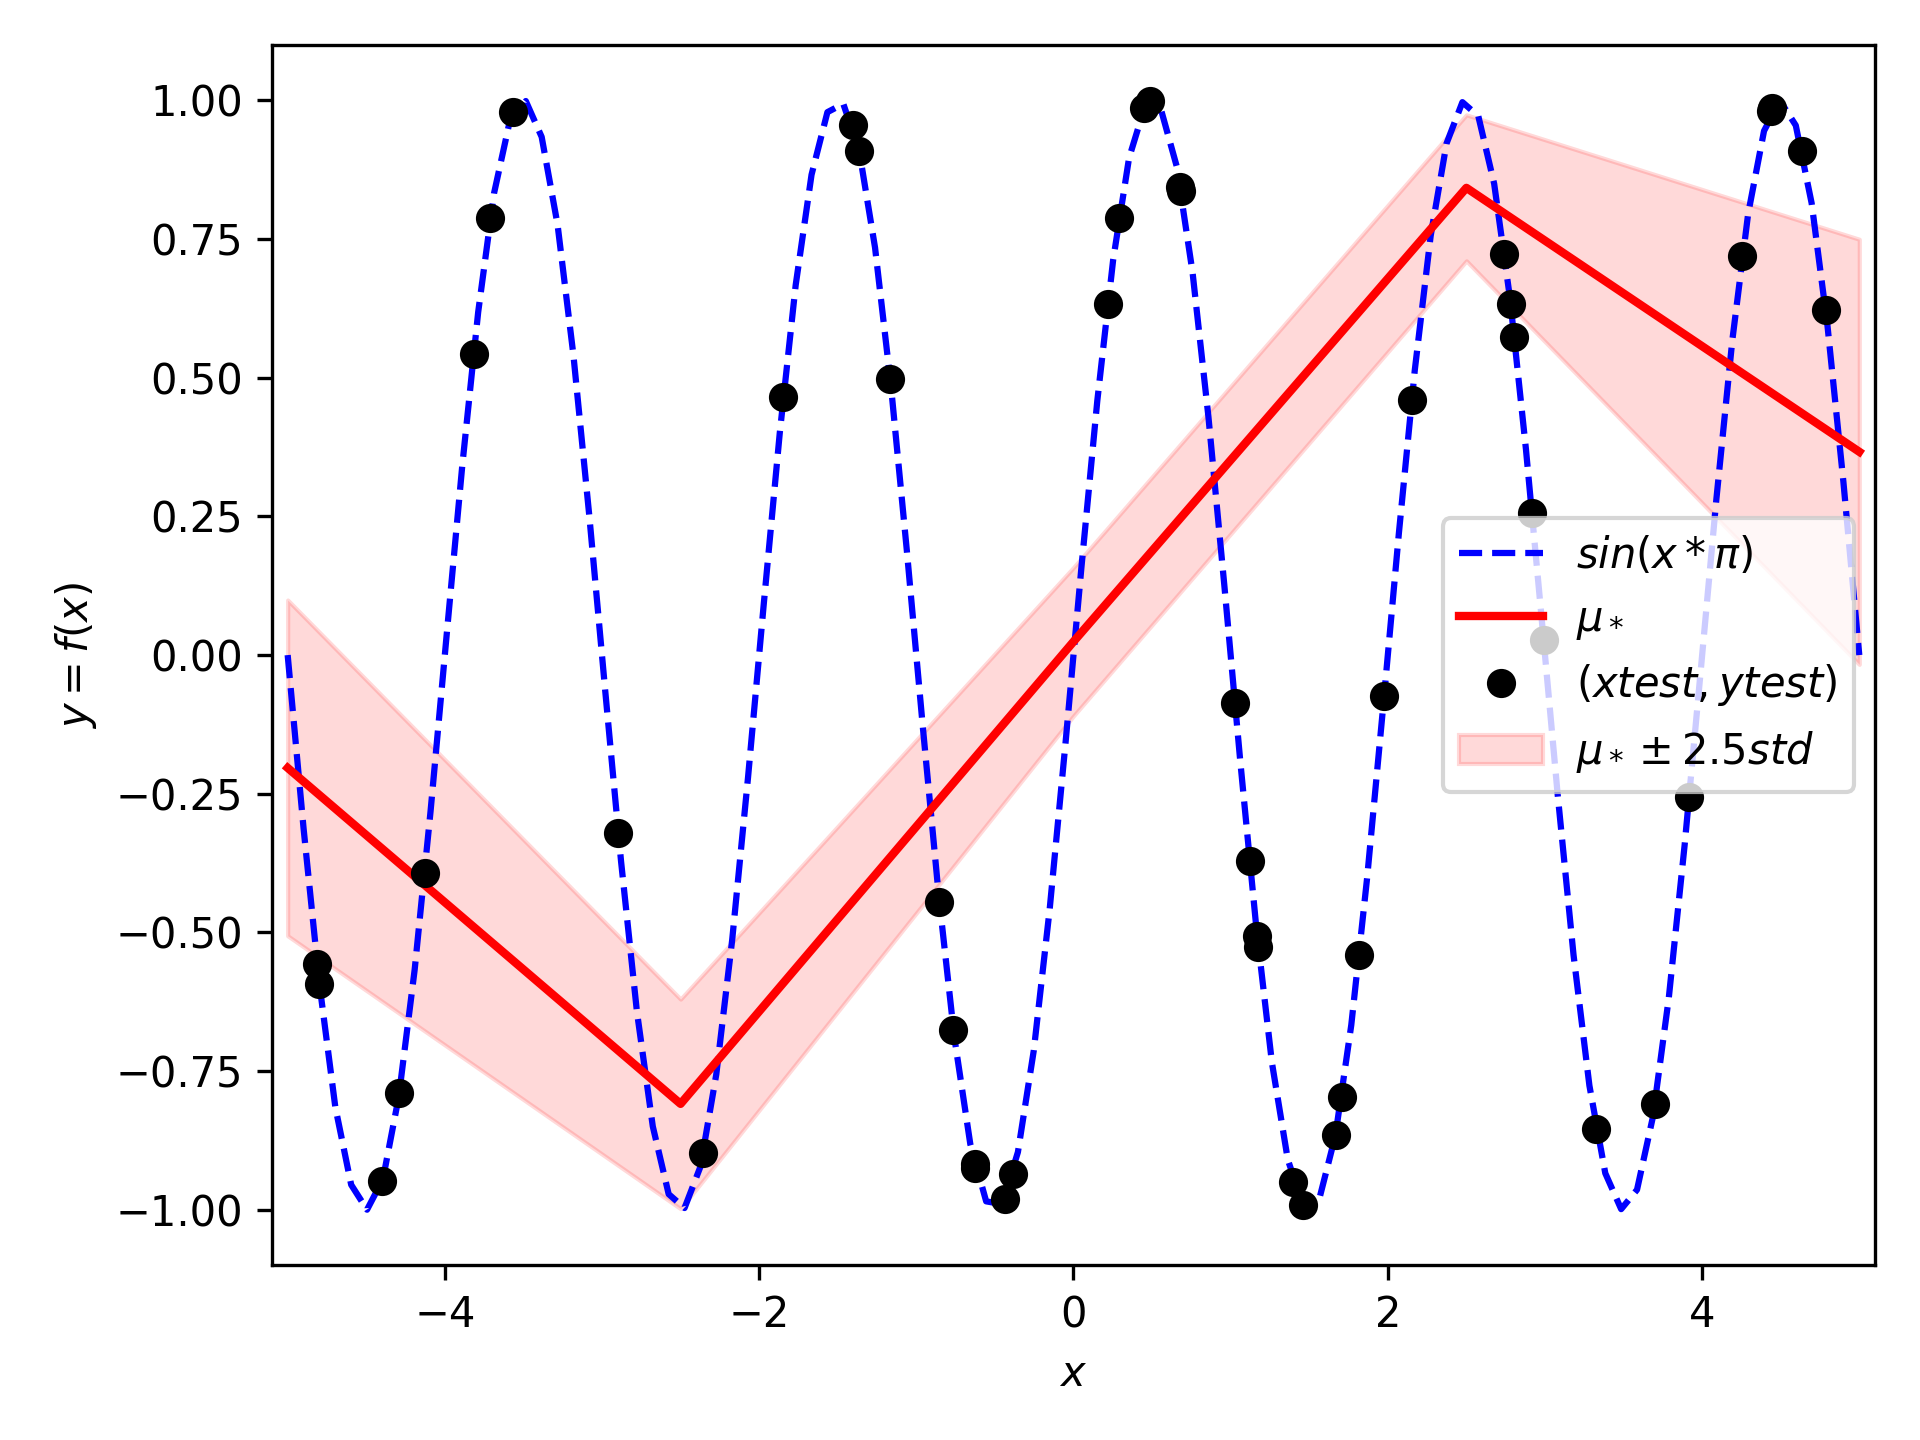
\includegraphics[width=\linewidth]{test_size/func1_5.png}
    \caption{$f_1; S = 5$}
  \end{subfigure}
  \begin{subfigure}{.33\textwidth}
    \centering
    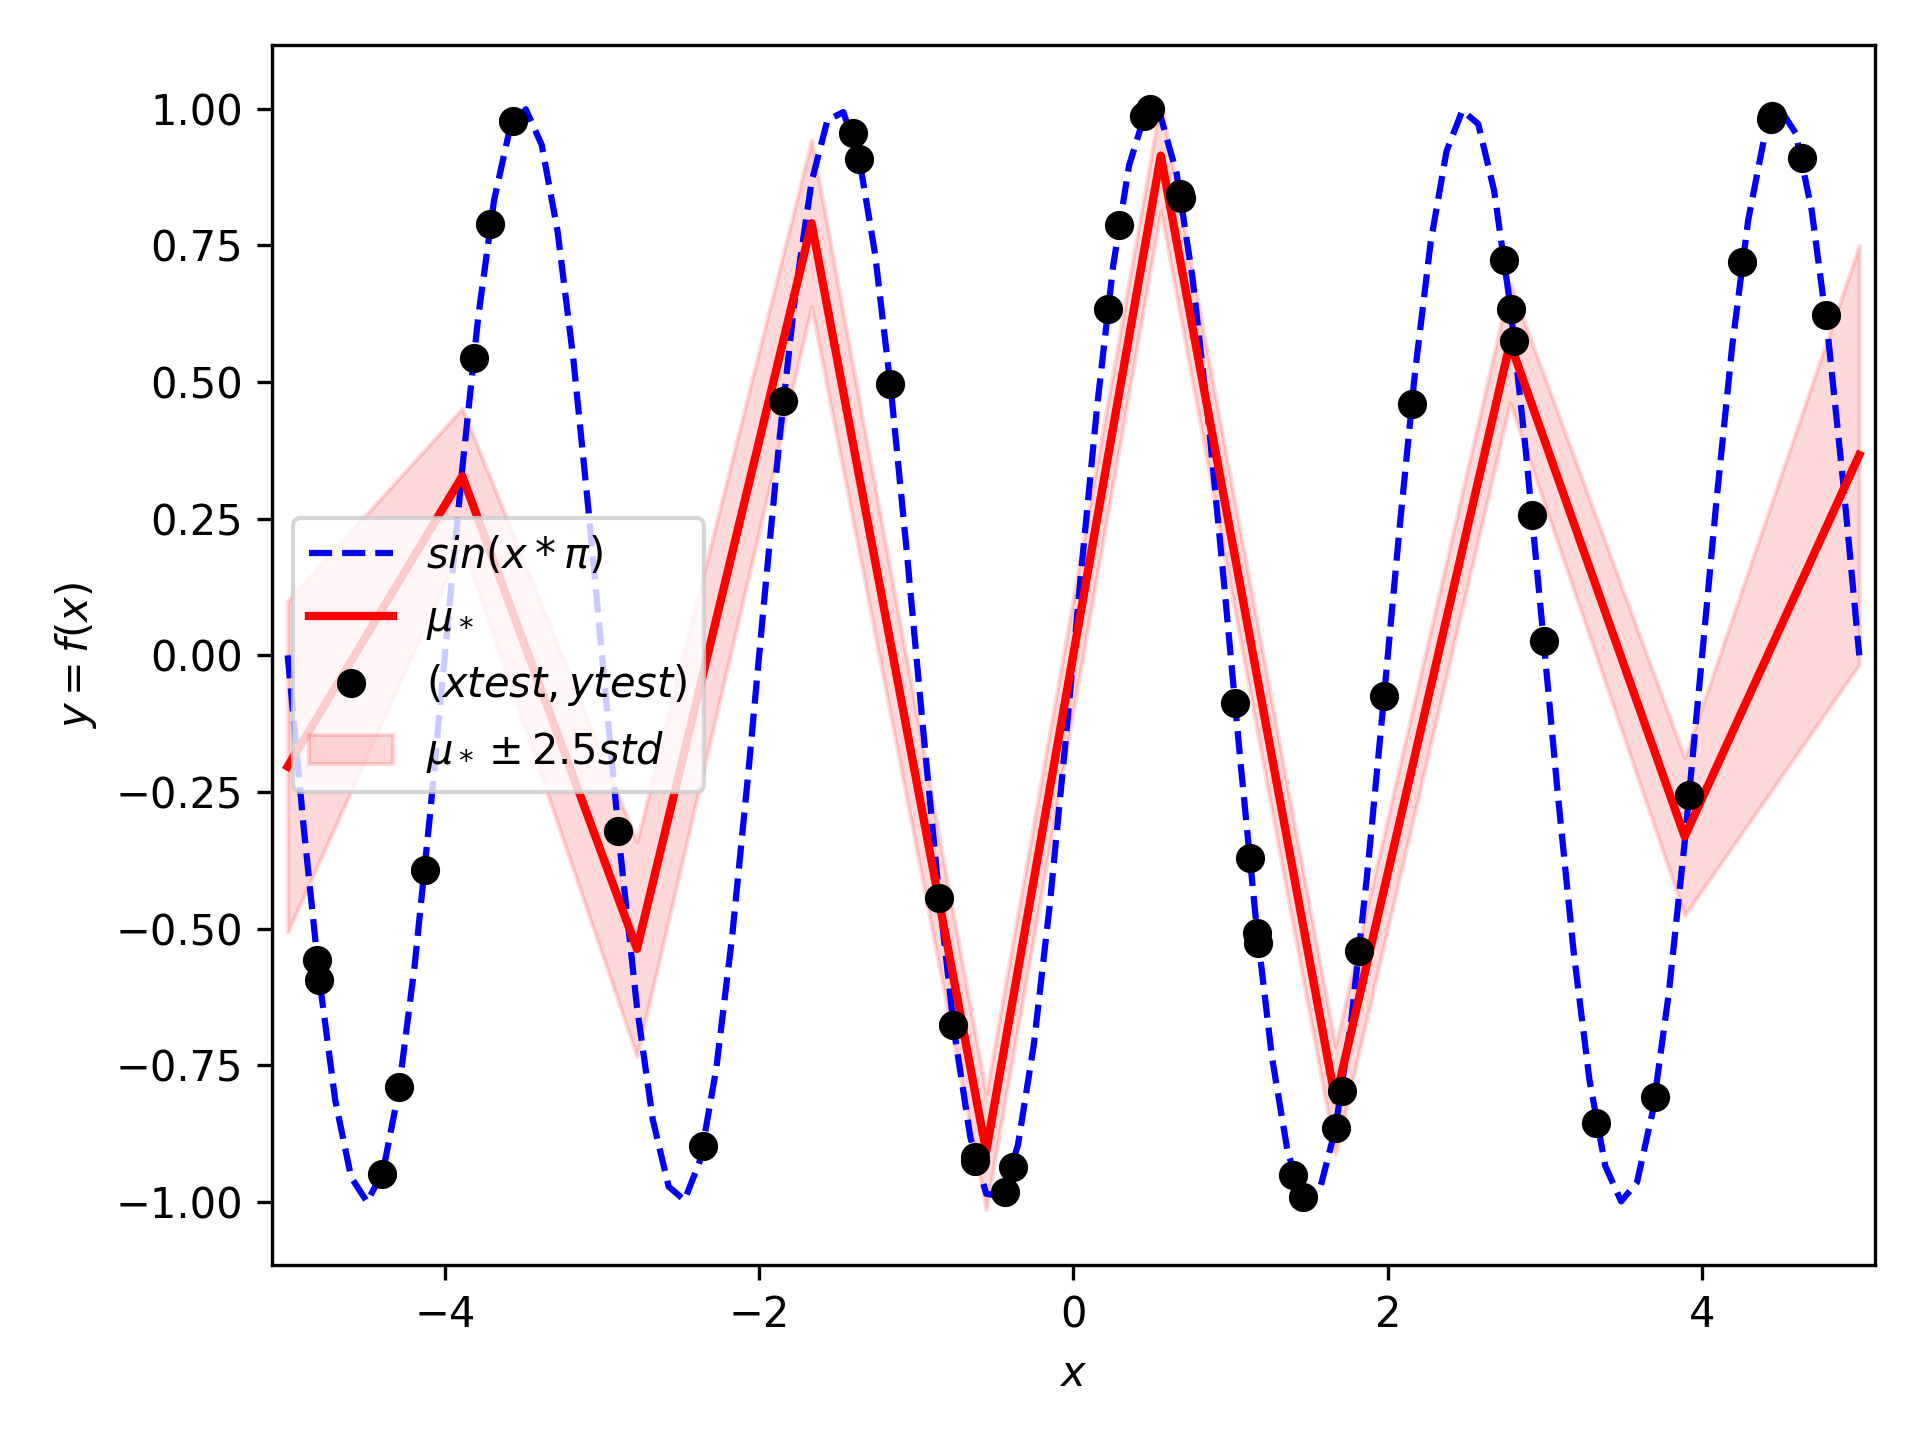
\includegraphics[width=\linewidth]{test_size/func1_10.png}
    \caption{$f_1; S = 10$}
  \end{subfigure}
  \begin{subfigure}{.33\textwidth}
    \centering
    \includegraphics[width=\linewidth]{test_size/func1_50.png}
    \caption{$f_1; S = 50$}
  \end{subfigure}
  \begin{subfigure}{.33\textwidth}
    \centering
    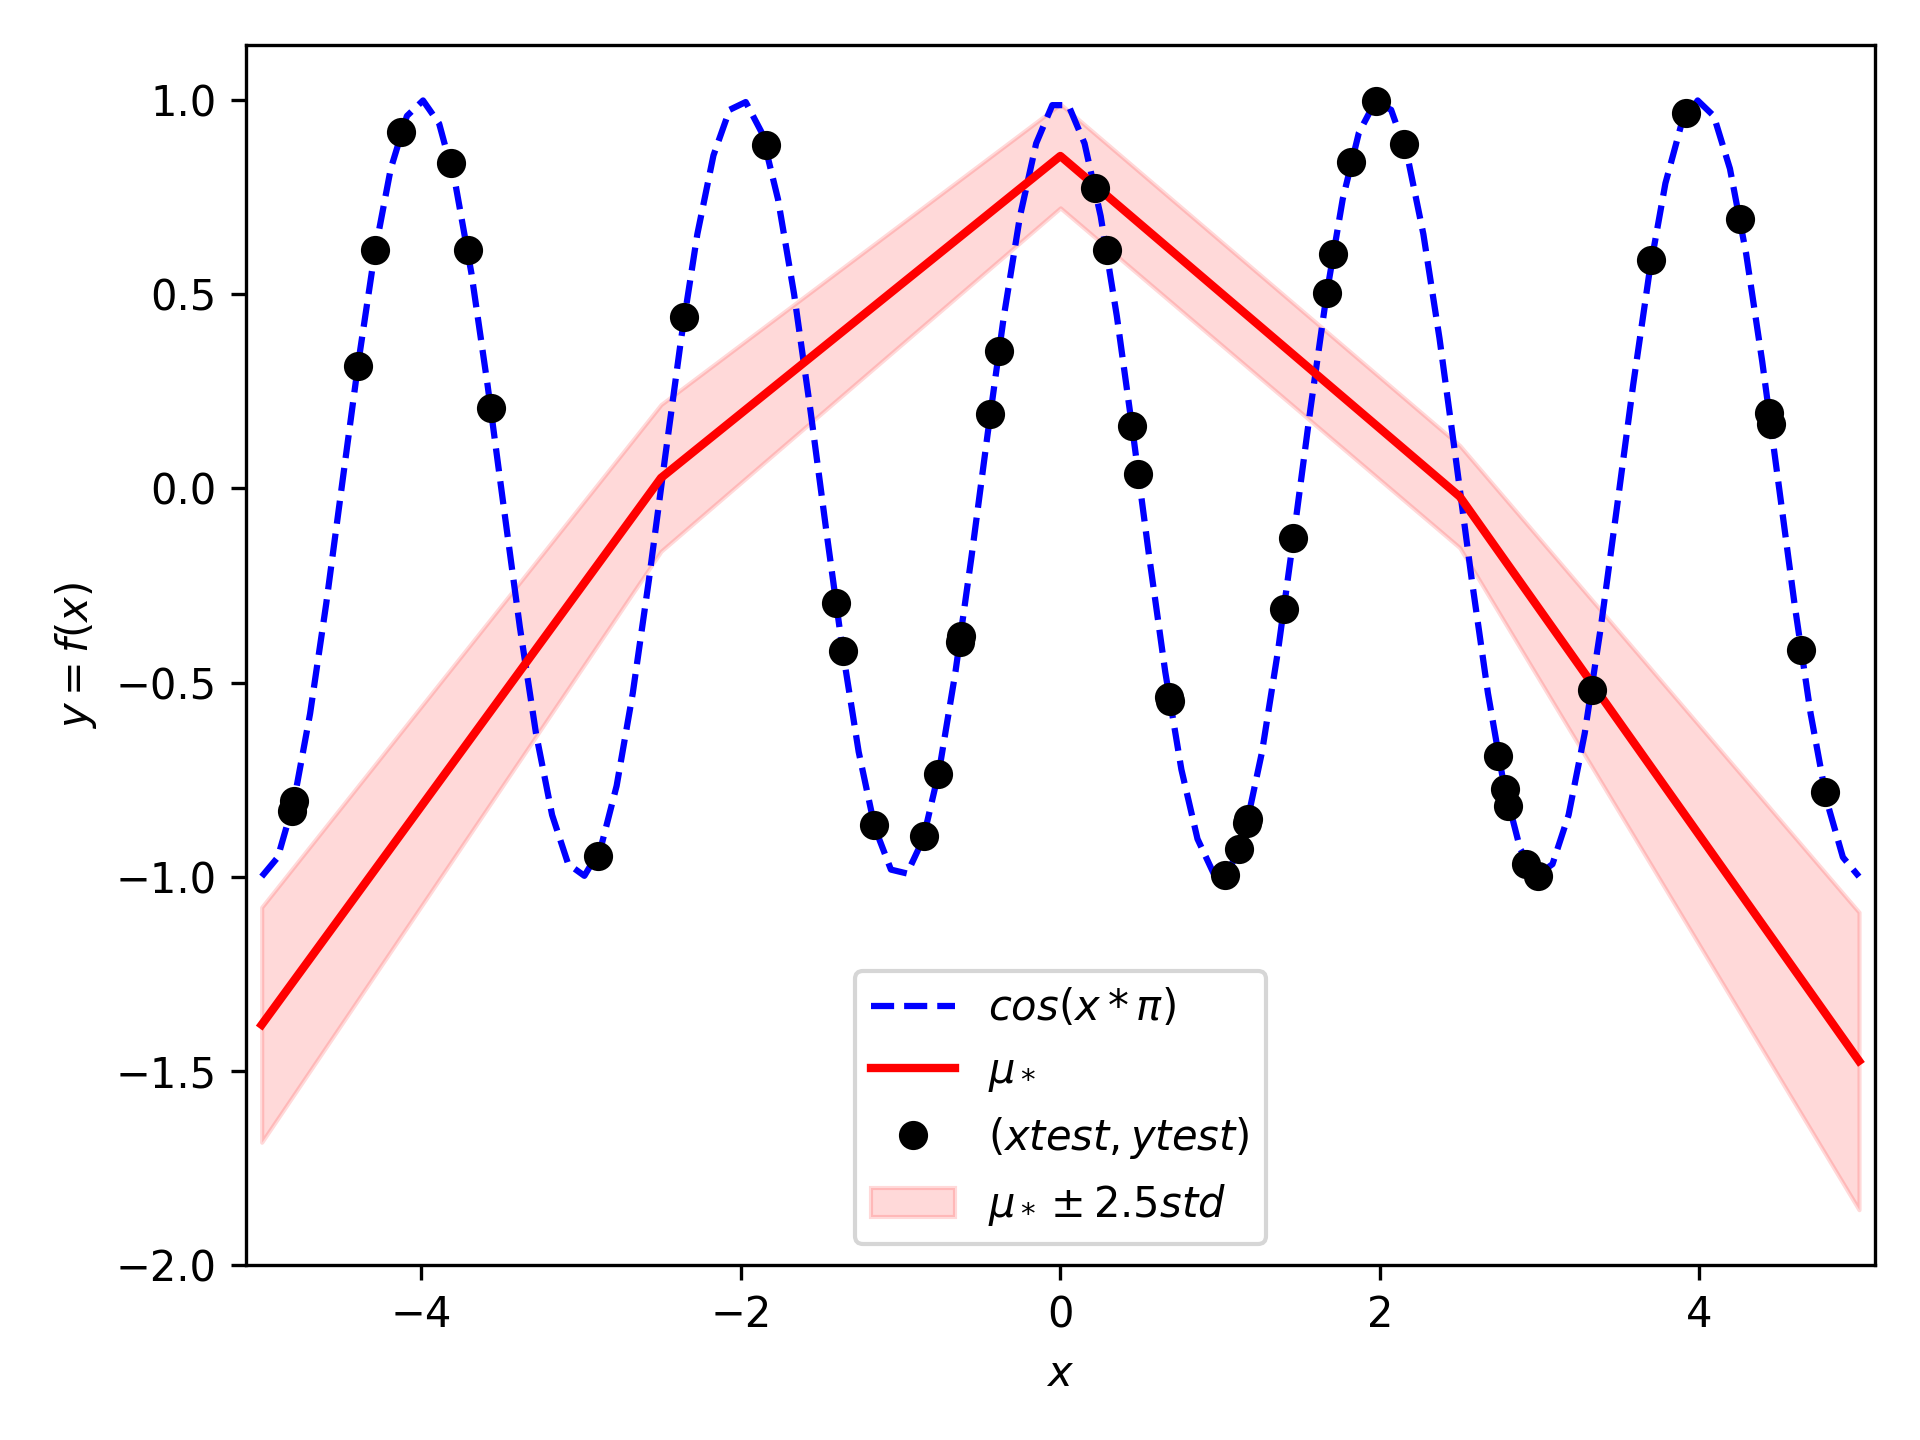
\includegraphics[width=\linewidth]{test_size/func2_5.png}
    \caption{$f_2; S = 5$}
  \end{subfigure}
  \begin{subfigure}{.33\textwidth}
    \centering
    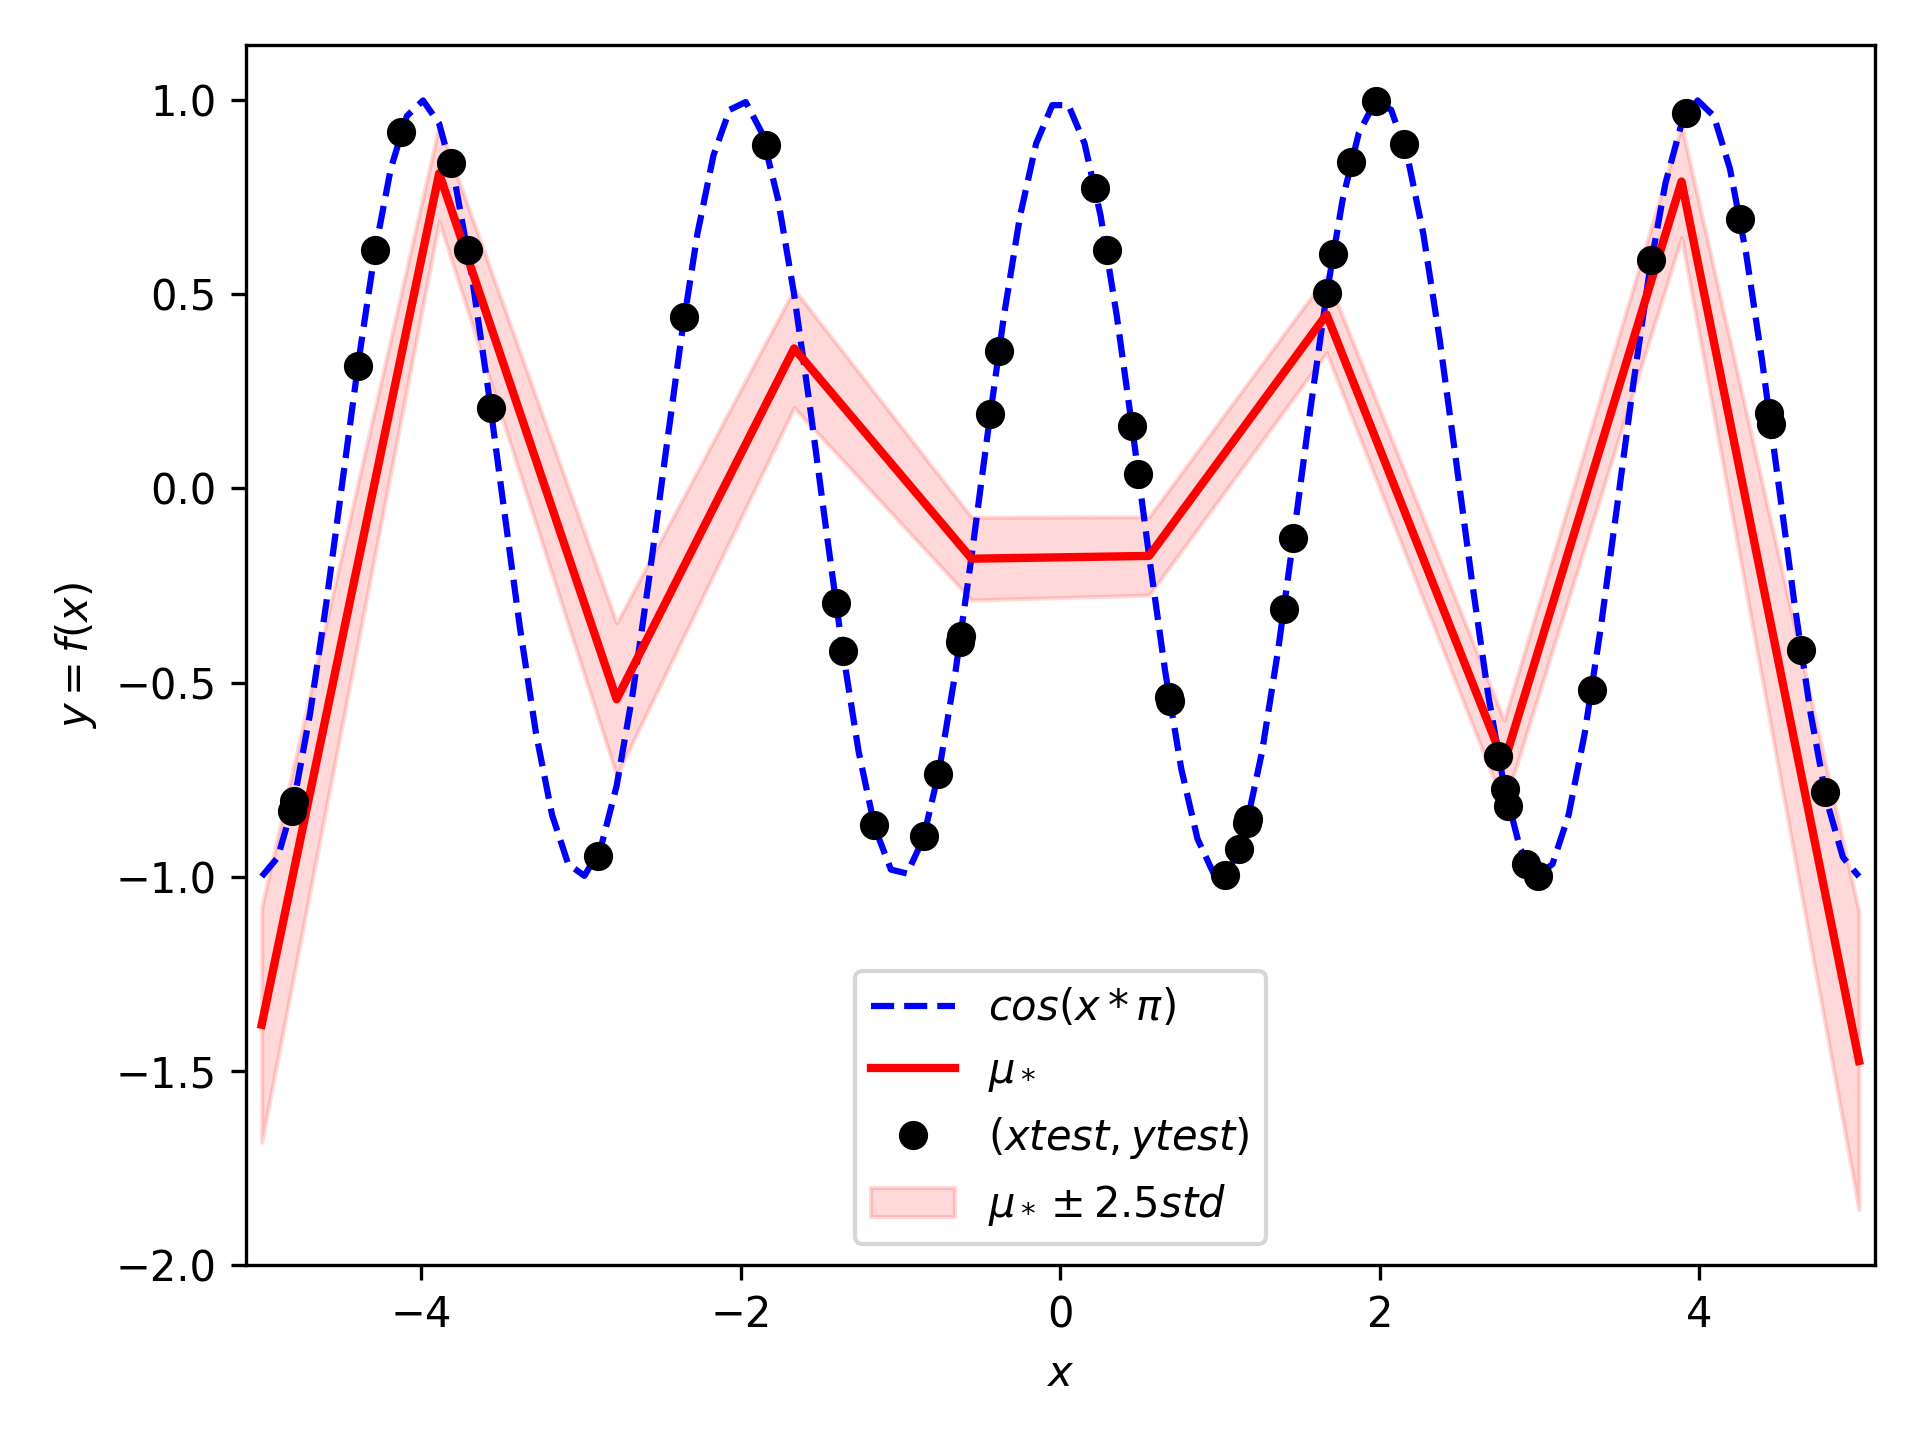
\includegraphics[width=\linewidth]{test_size/func2_10.png}
    \caption{$f_2; S = 10$}
  \end{subfigure}
  \begin{subfigure}{.33\textwidth}
    \centering
    \includegraphics[width=\linewidth]{test_size/func2_50.png}
    \caption{$f_2; S = 50$}
  \end{subfigure}
  \begin{subfigure}{.33\textwidth}
    \centering
    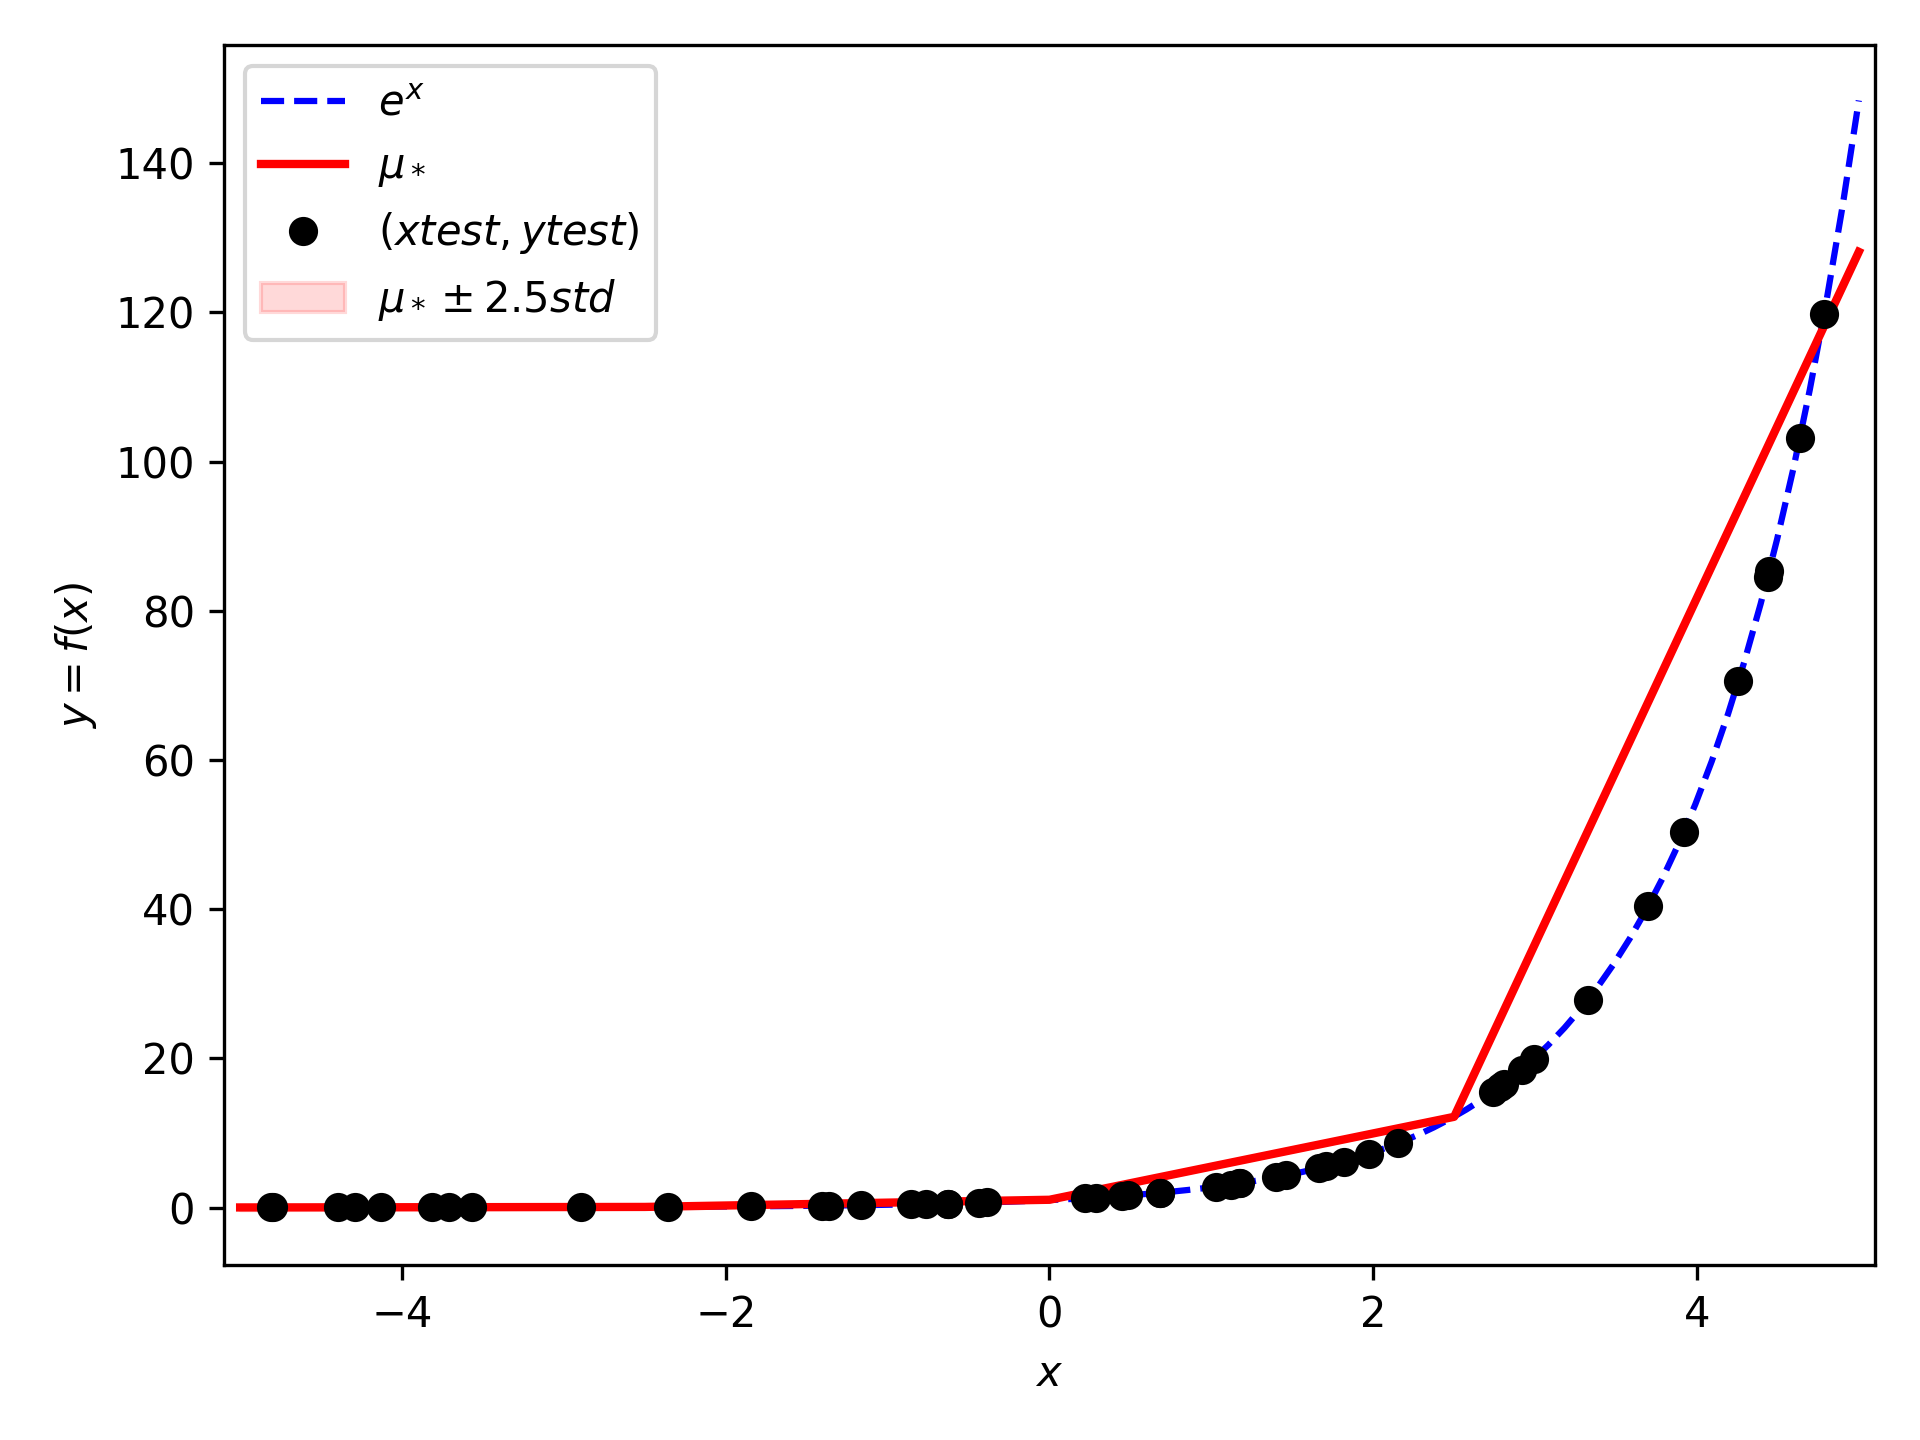
\includegraphics[width=\linewidth]{test_size/func3_5.png}
    \caption{$f_3; S = 5$}
  \end{subfigure}
  \begin{subfigure}{.33\textwidth}
    \centering
    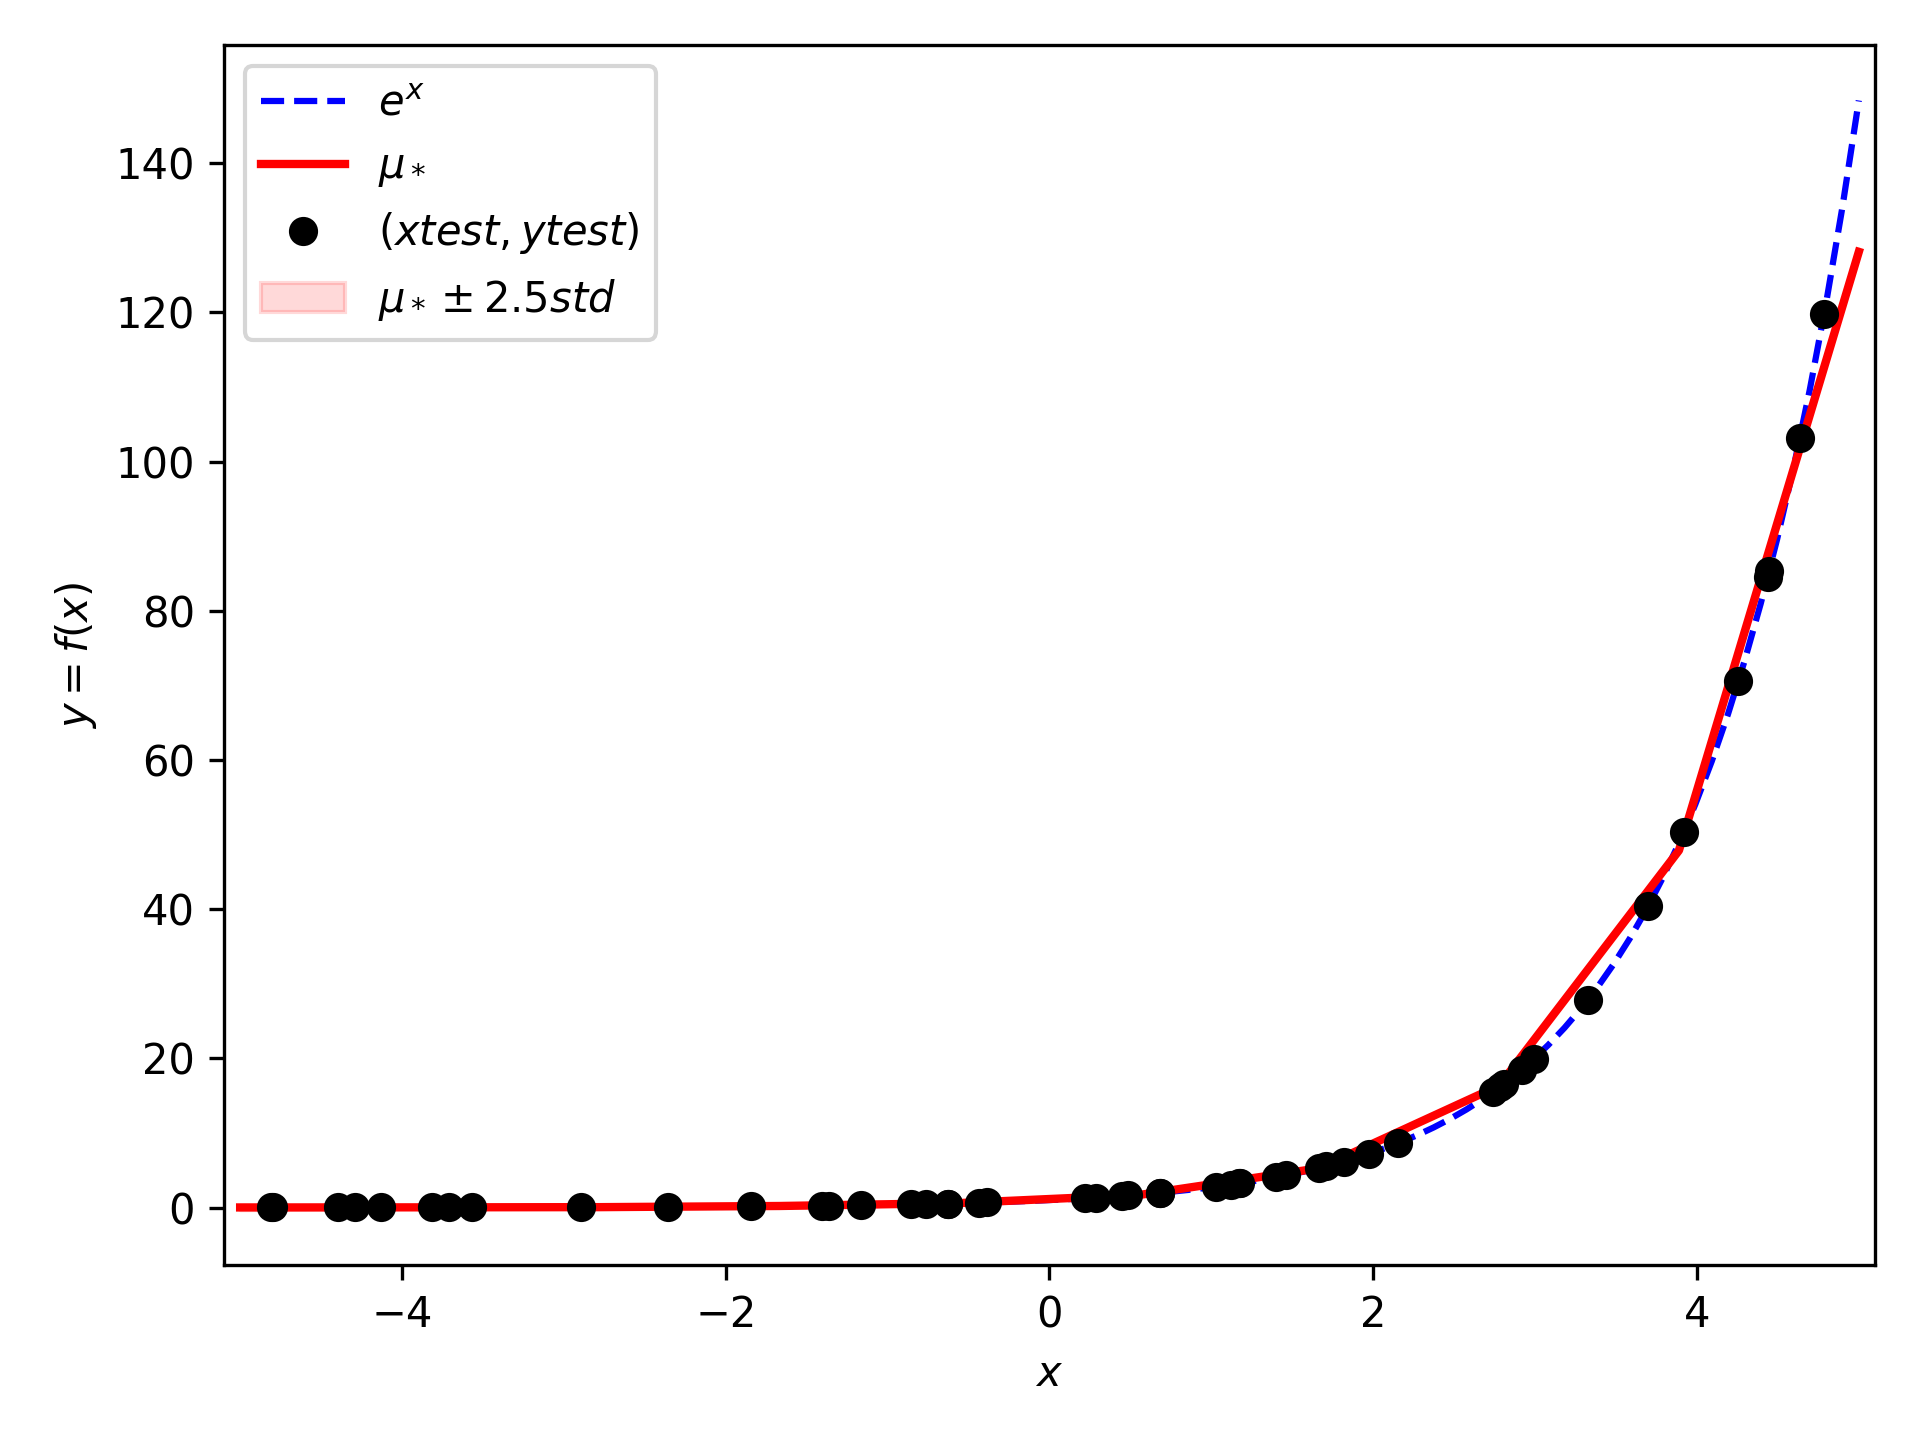
\includegraphics[width=\linewidth]{test_size/func3_10.png}
    \caption{$f_3; S = 10$}
  \end{subfigure}
  \begin{subfigure}{.33\textwidth}
    \centering
    \includegraphics[width=\linewidth]{test_size/func3_50.png}
    \caption{$f_3; S = 50$}
  \end{subfigure}
  \caption{Gaussian Processes with SE kernel with different test set sizes (S). The samples comes from three different functions (sine - $f_1$, cosine - $f_2$ and exponential - $f_3$).}
  \label{fig:test_samples}
  \end{figure}

\subsection{Effect of kernel parameters}

Here, we evaluate the different values for the kernel parameters: $\sigma$, $\ell$ and $\sigma_y^2$. All experiments in this section used 50 samples in the training and test sets, using the function sine as the target function.

\subsubsection{Parameters $\ell$}

We evaluated effects of the parameters $\ell$ of the SE kernel (Eq.\eqref{eq:kernelSE}) on our predictions, keeping the remaing parameters ($\sigma$ and $\sigma_y^2$) in their default value (Fig. \ref{fig:ell}).

As known, the parameter $\ell$ is the horizontal scale over which the target function changes. Based on Fig. \ref{fig:ell}, we observed that $\ell = 1$ is closer to the optimum value of the parameter. If we decrease its value, the curve becomes more wiggly and the uncertainty also increases (\ie wider confidence interval), since the effective distance from the training set samples increases more quickly. However, if we increase its value, it becomes smoother until it becomes a straight line. 

\begin{figure}[h]
  \begin{subfigure}{.33\textwidth}
    \centering
    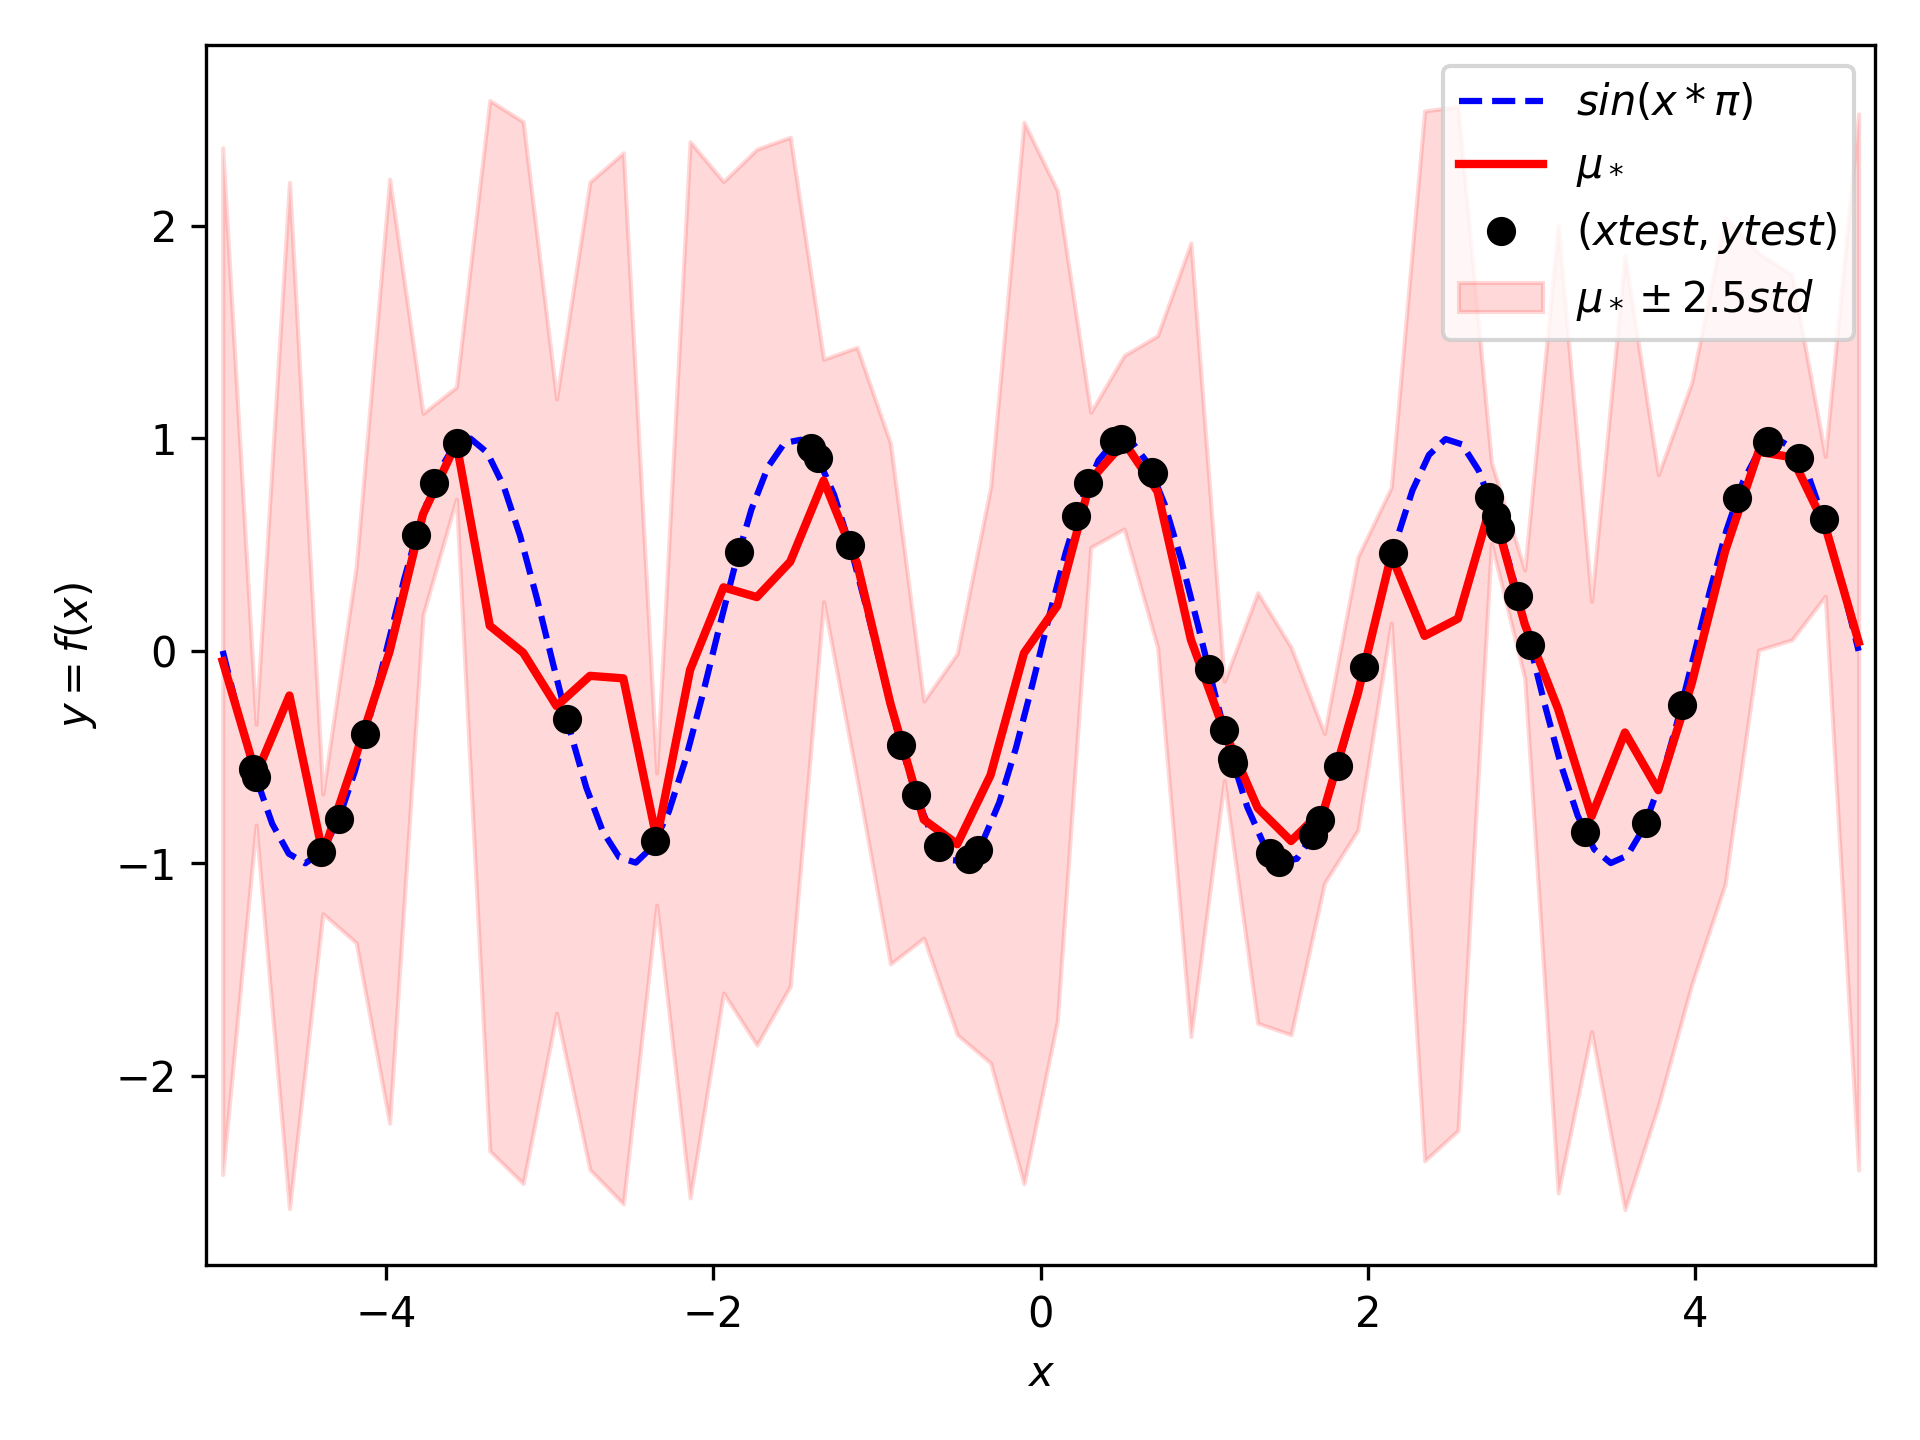
\includegraphics[width=\linewidth]{kernelSE/ell/0_1.png}
    \caption{$\ell = 0.1$}
    \label{fig:ell01}
  \end{subfigure}
  \begin{subfigure}{.33\textwidth}
    \centering
    \includegraphics[width=\linewidth]{kernelSE/ell/1.png}
    \caption{$\ell = 1$}
    \label{fig:ell1}
  \end{subfigure}
  \begin{subfigure}{.33\textwidth}
    \centering
    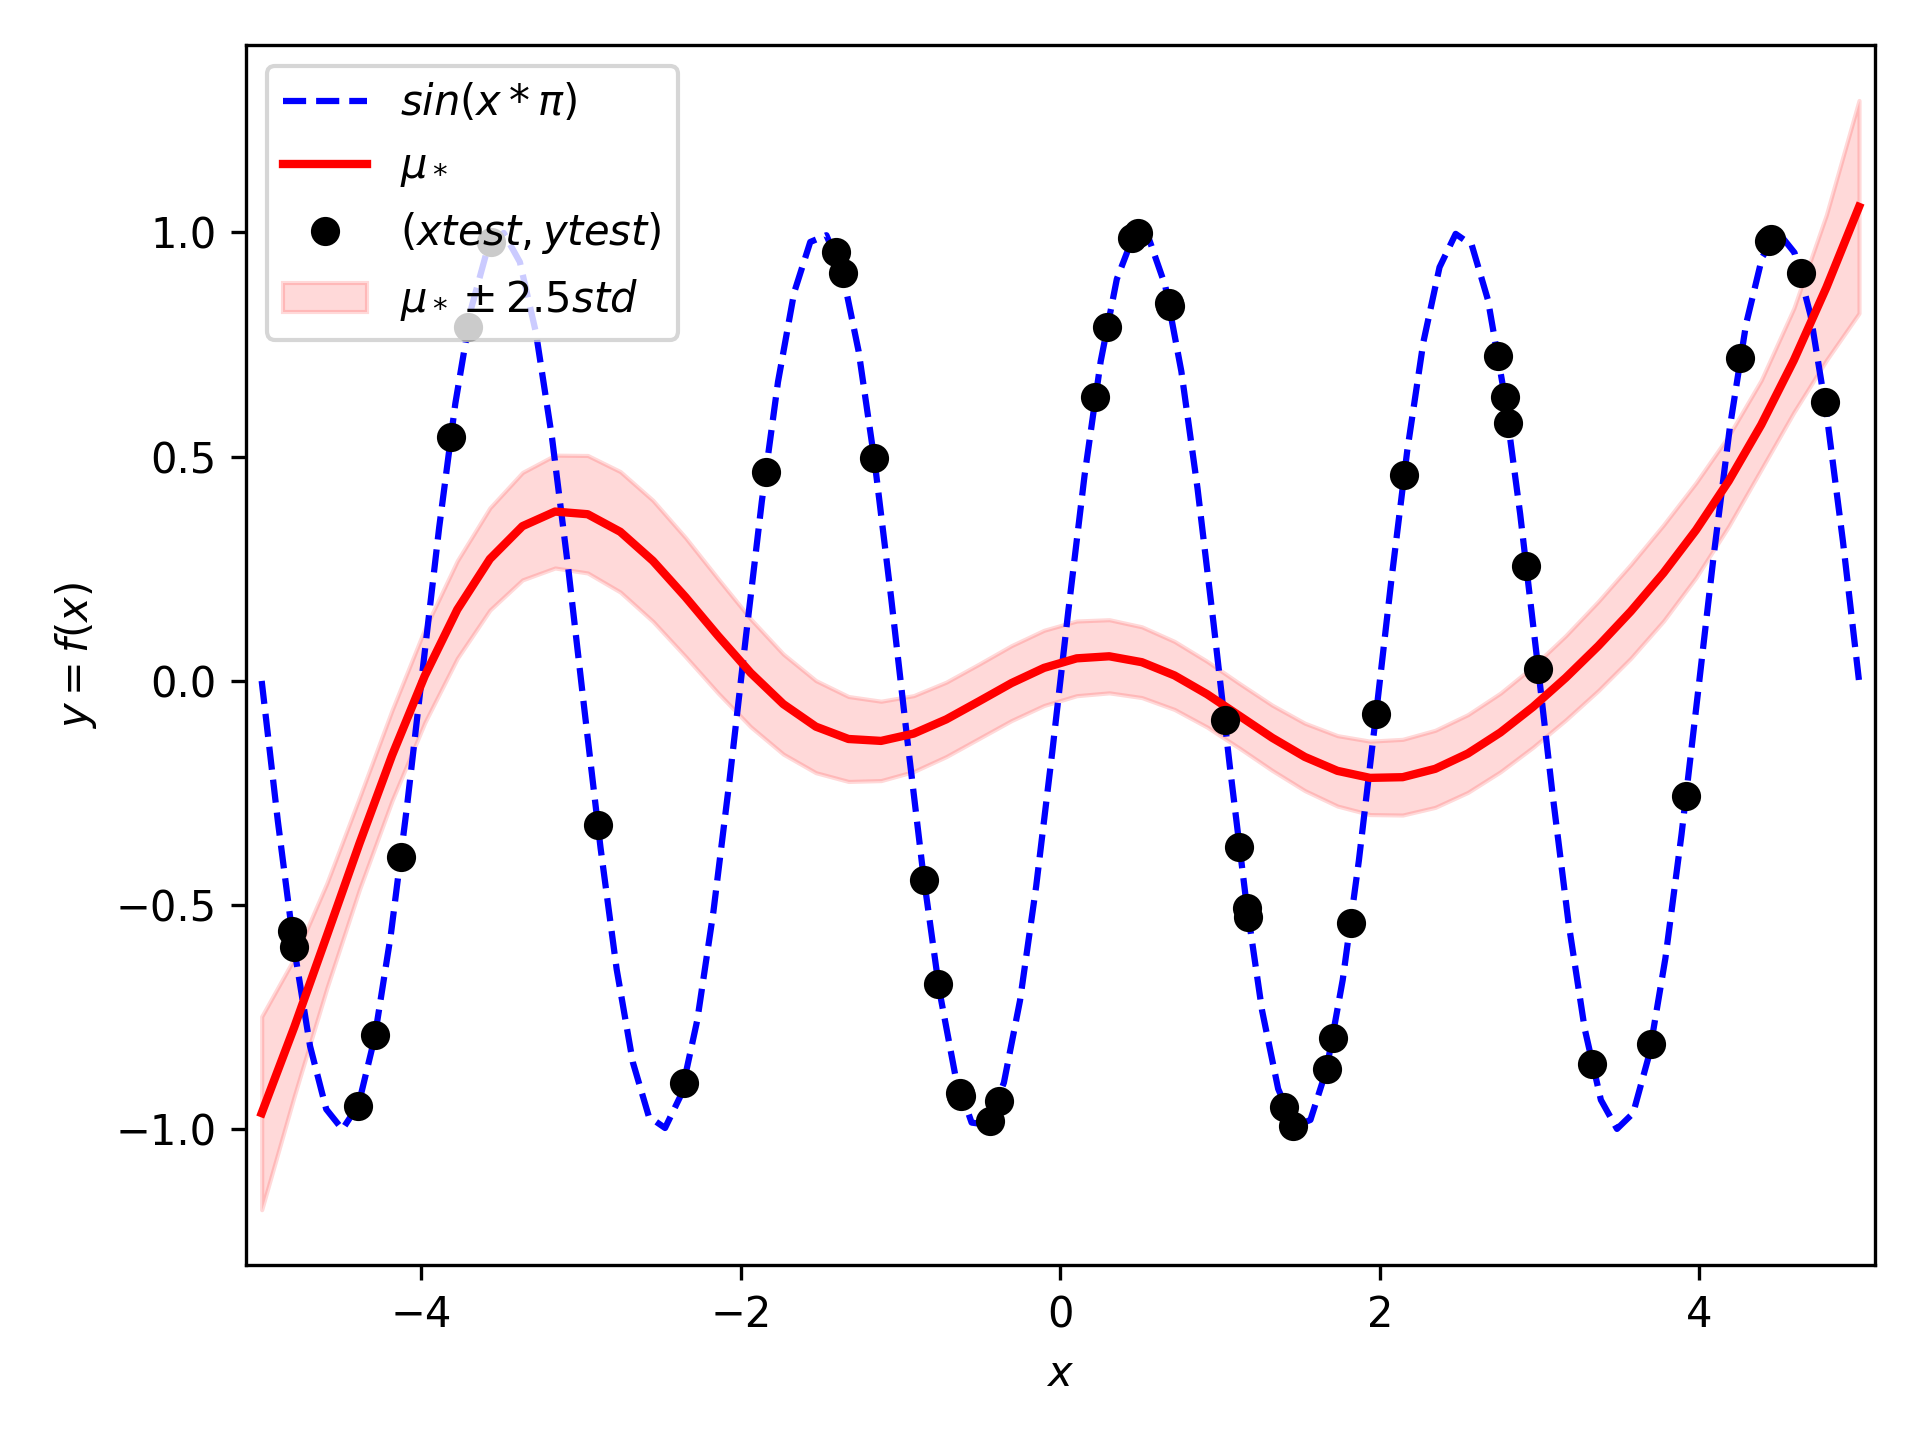
\includegraphics[width=\linewidth]{kernelSE/ell/2.png}
    \caption{$\ell = 2$}
    \label{fig:ell2}
  \end{subfigure}
  \begin{subfigure}{.33\textwidth}
    \centering
    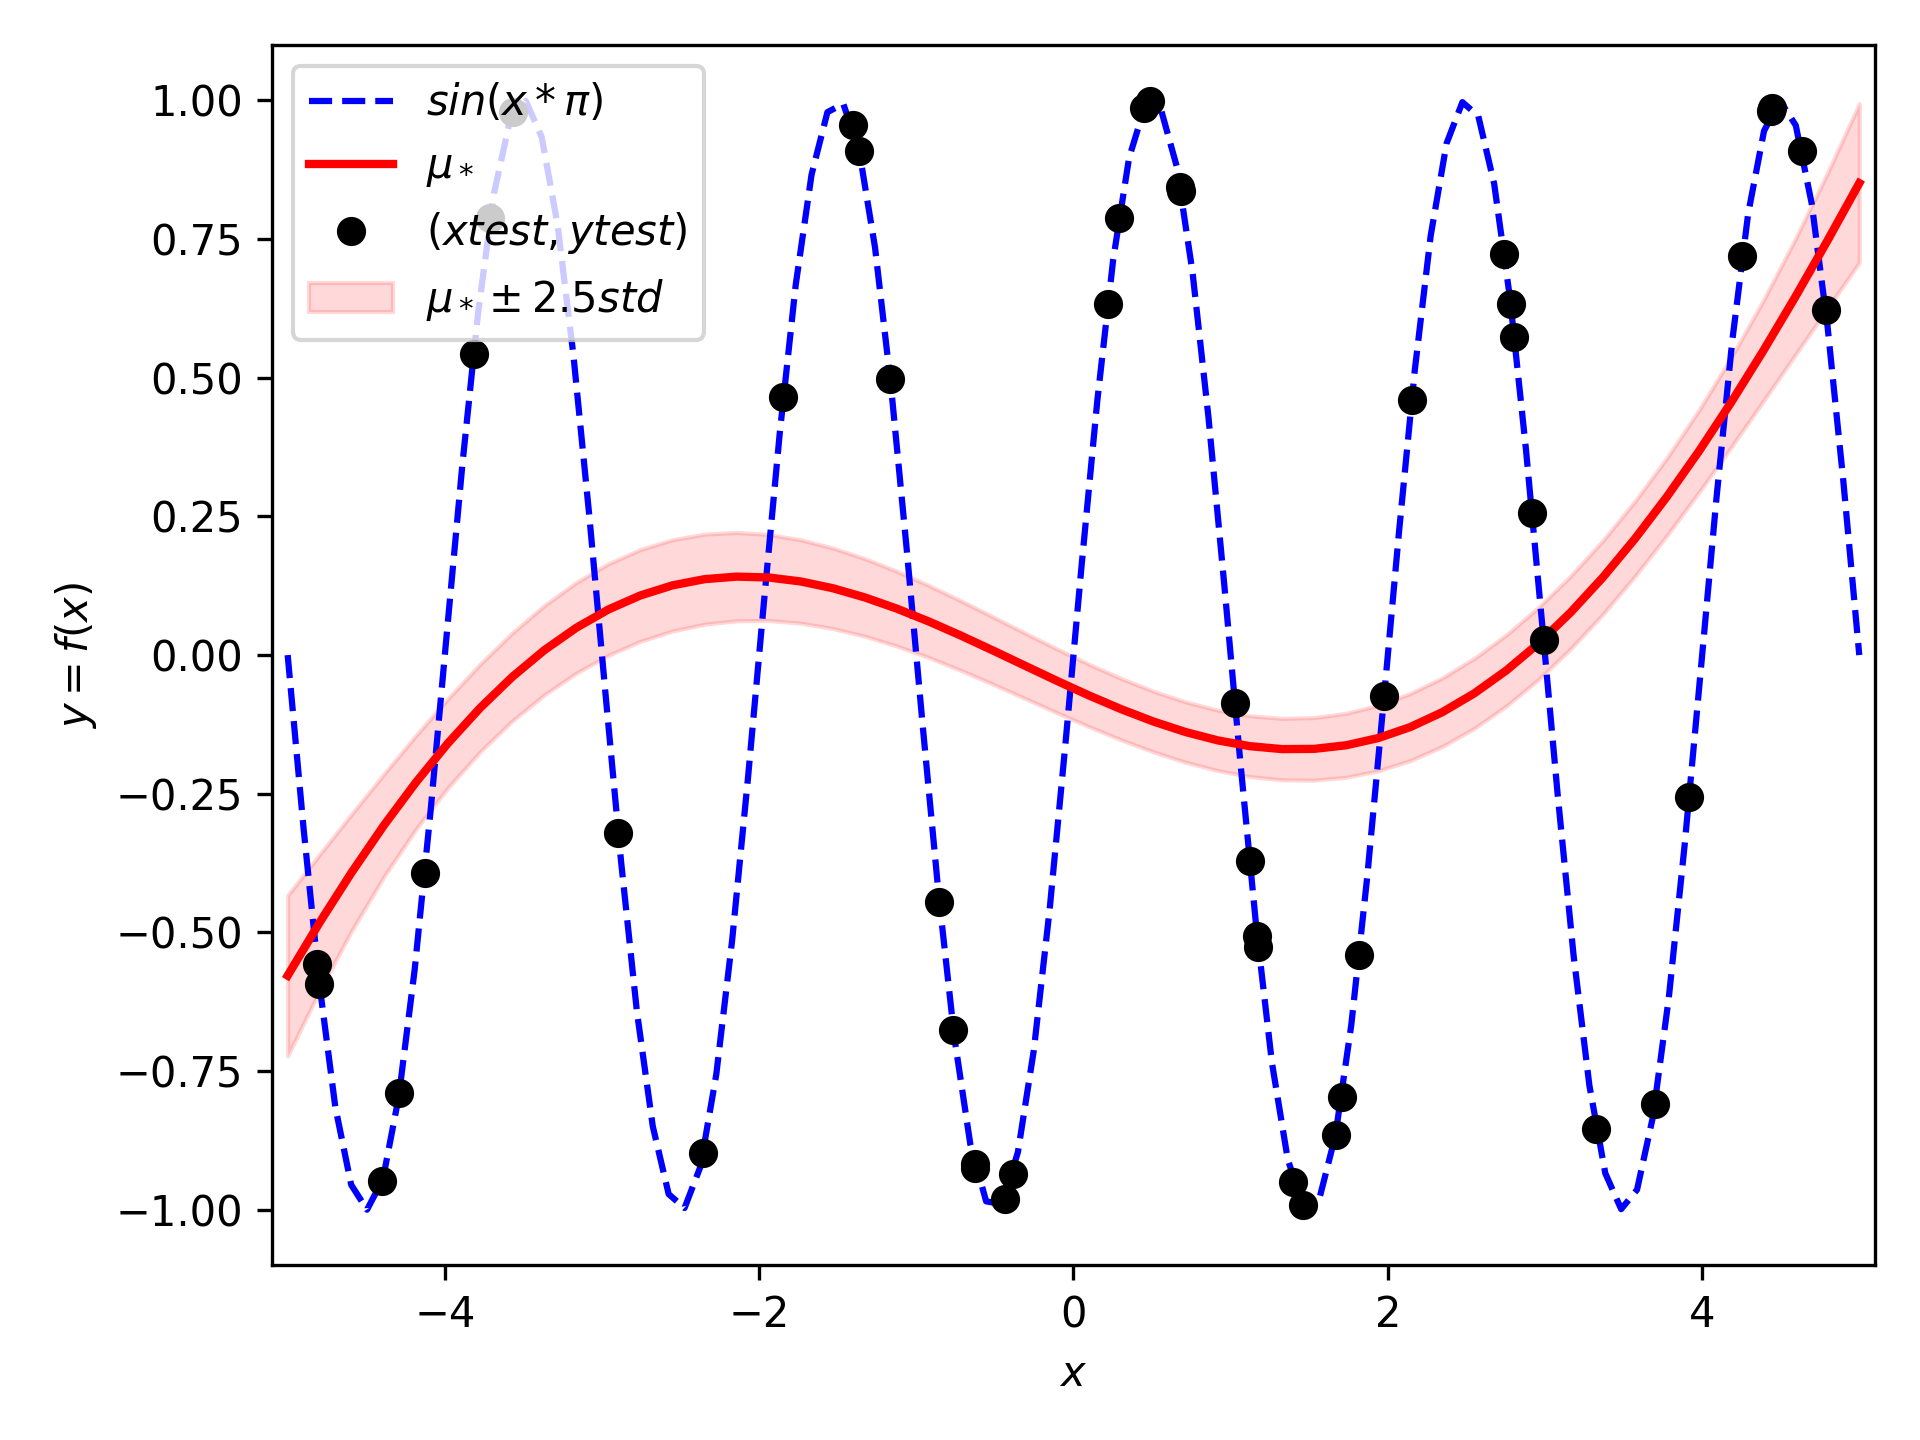
\includegraphics[width=\linewidth]{kernelSE/ell/5.png}
    \caption{$\ell = 5$}
    \label{fig:ell5}
  \end{subfigure}
  \begin{subfigure}{.33\textwidth}
    \centering
    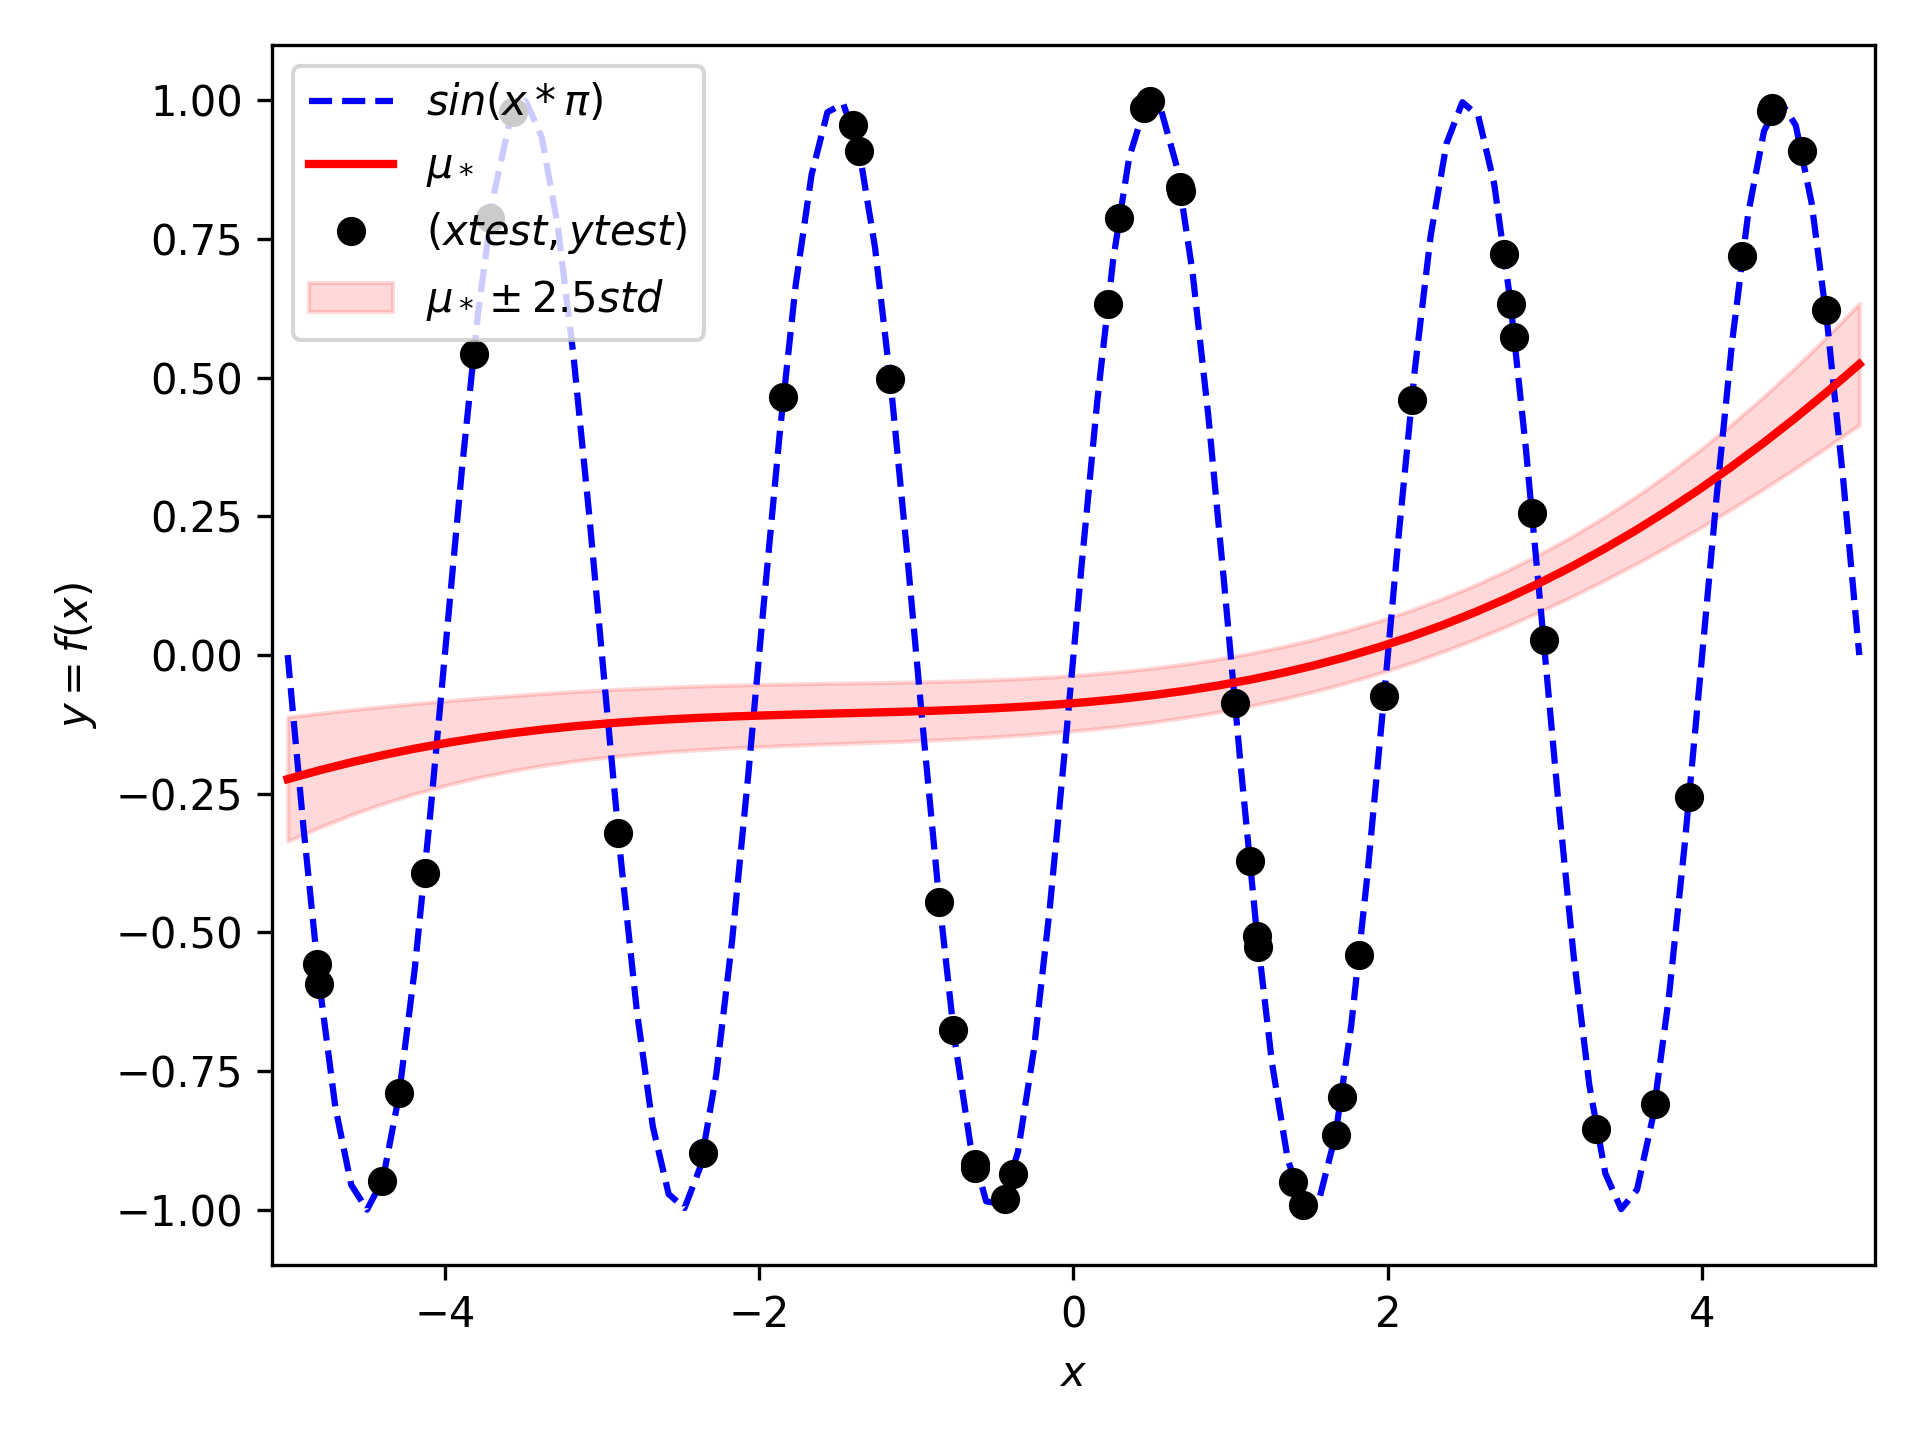
\includegraphics[width=\linewidth]{kernelSE/ell/10.png}
    \caption{$\ell = 10$}
    \label{fig:ell10}
  \end{subfigure}
  \begin{subfigure}{.33\textwidth}
    \centering
    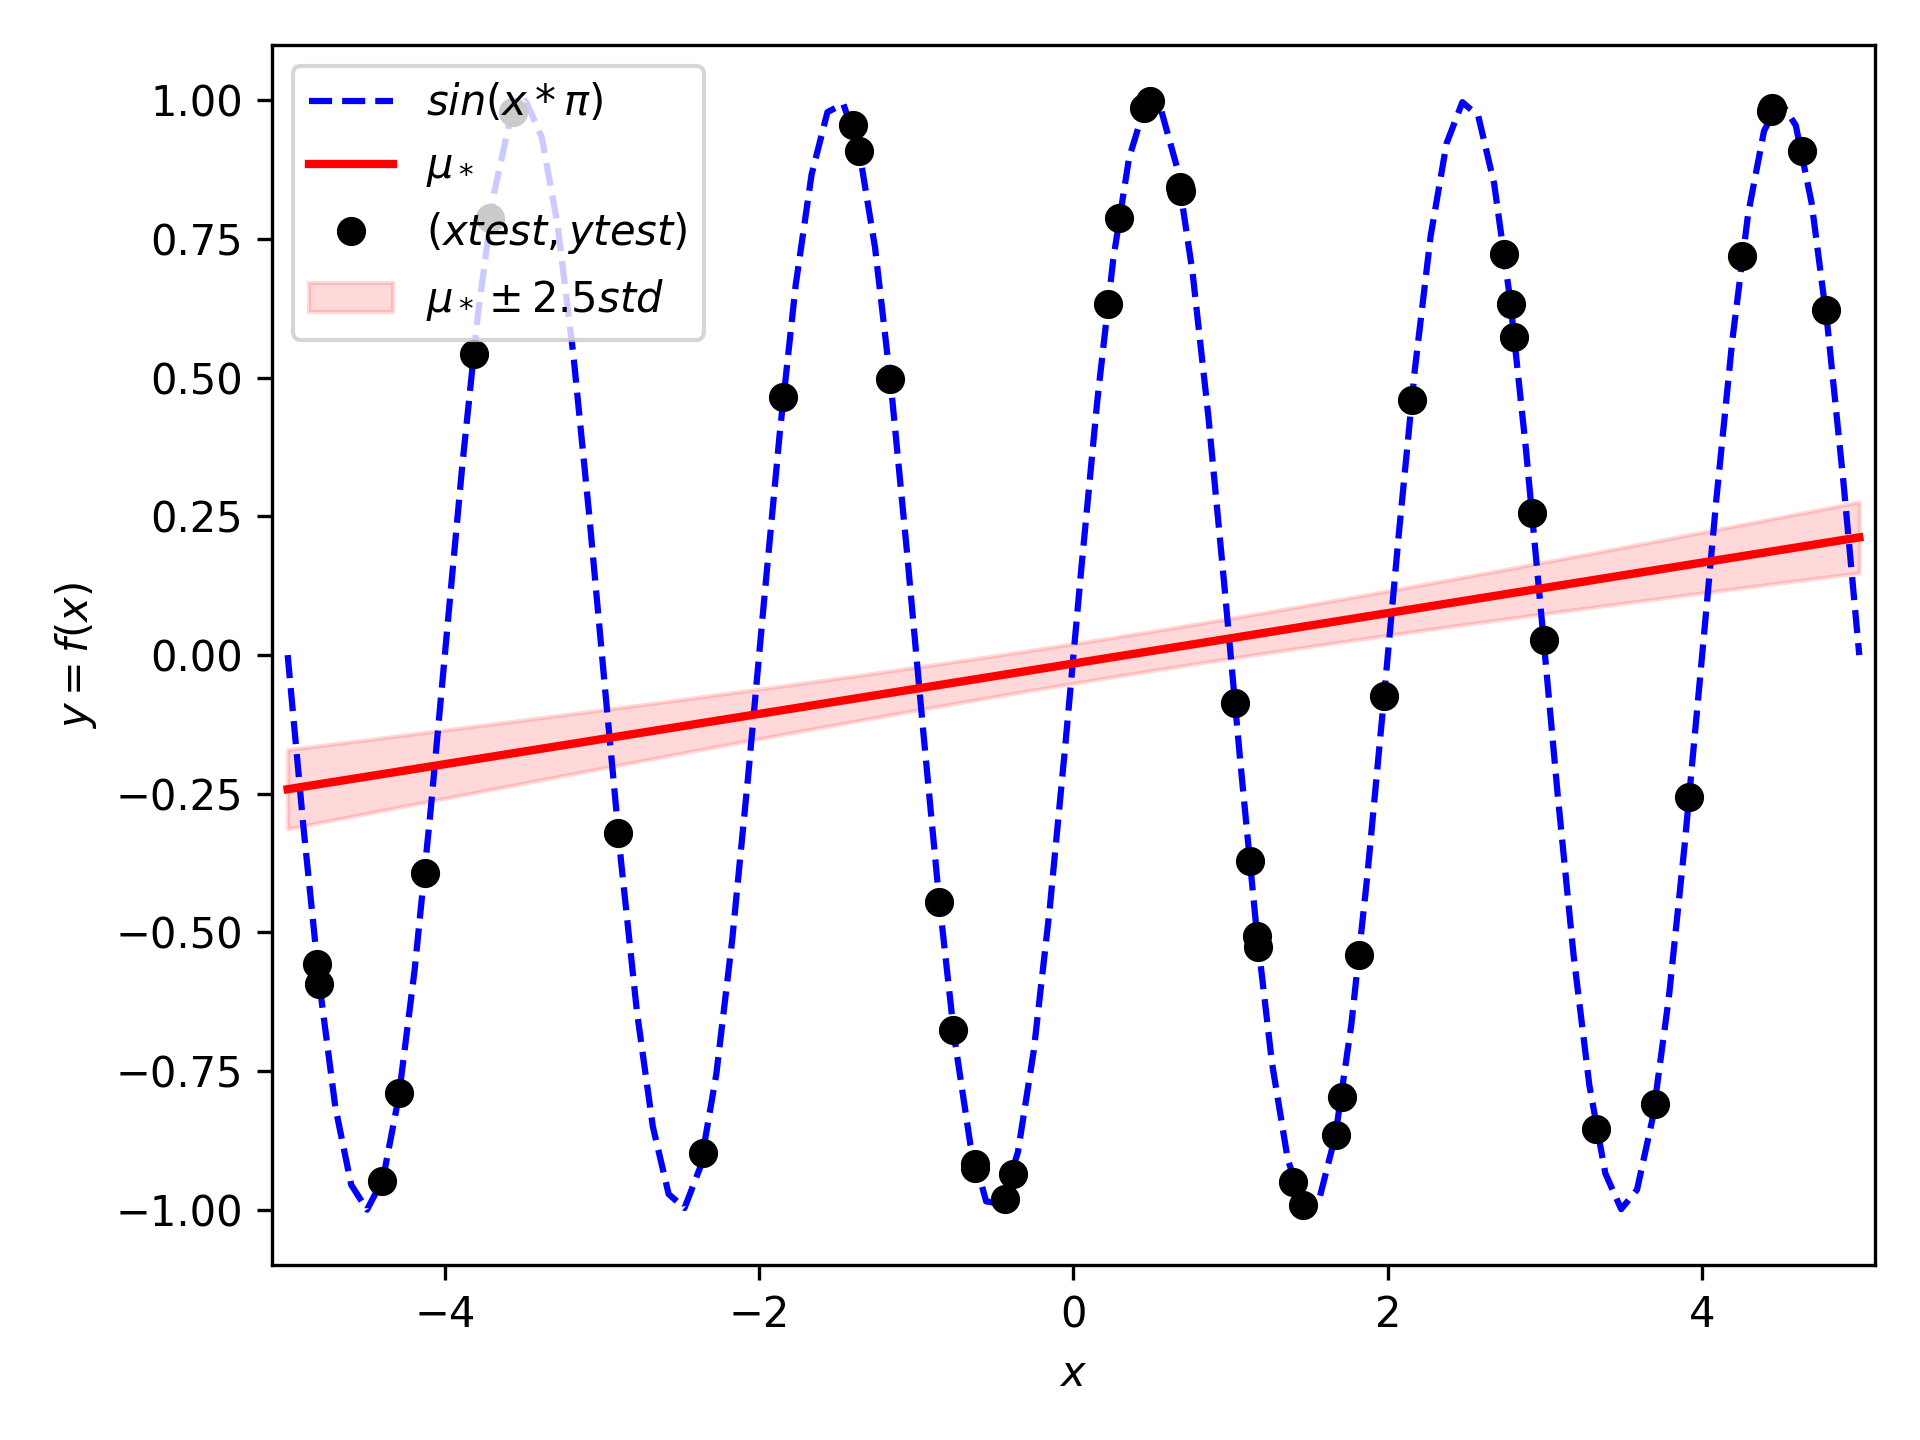
\includegraphics[width=\linewidth]{kernelSE/ell/100.png}
    \caption{$\ell = 100$}
    \label{fig:ell100}
  \end{subfigure}
  \caption{Gaussian Processes with SE kernel with different values of $\ell$. The remaining parameters of SE kernel are fixed ($\sigma = 1$ and $\sigma_y^2 = 0.01$).}
  \label{fig:ell}
\end{figure}

\subsubsection{Parameters $\sigma$}

We evaluated effects of the parameters $\sigma$ of the SE kernel (Eq.\eqref{eq:kernelSE}) on our predictions, keeping the remaing parameters ($\ell$ and $\sigma_y^2$) in their default value (Fig. \ref{fig:sigma}).

As we know, the parameter $\sigma$ is the vertical scale of the target function. Based on Fig. \ref{fig:sigma}, we observed that $\sigma = 1$ is closer to the optimum value of the parameter. If we decrease its value, the curve becomes smoother, until it becomes a straight line, and the uncertainty also decreases (\ie smaller confidence interval). On the other hand, if we increase its value, the regions where there are not training samples had an increase on their uncertainty (\ie wider confidence interval), this can be seen more clearly in the borders. Even so, there is a smaller increase in regions within the curve.

% sigma
\begin{figure}[ht]
  \begin{subfigure}{.33\textwidth}
    \centering
    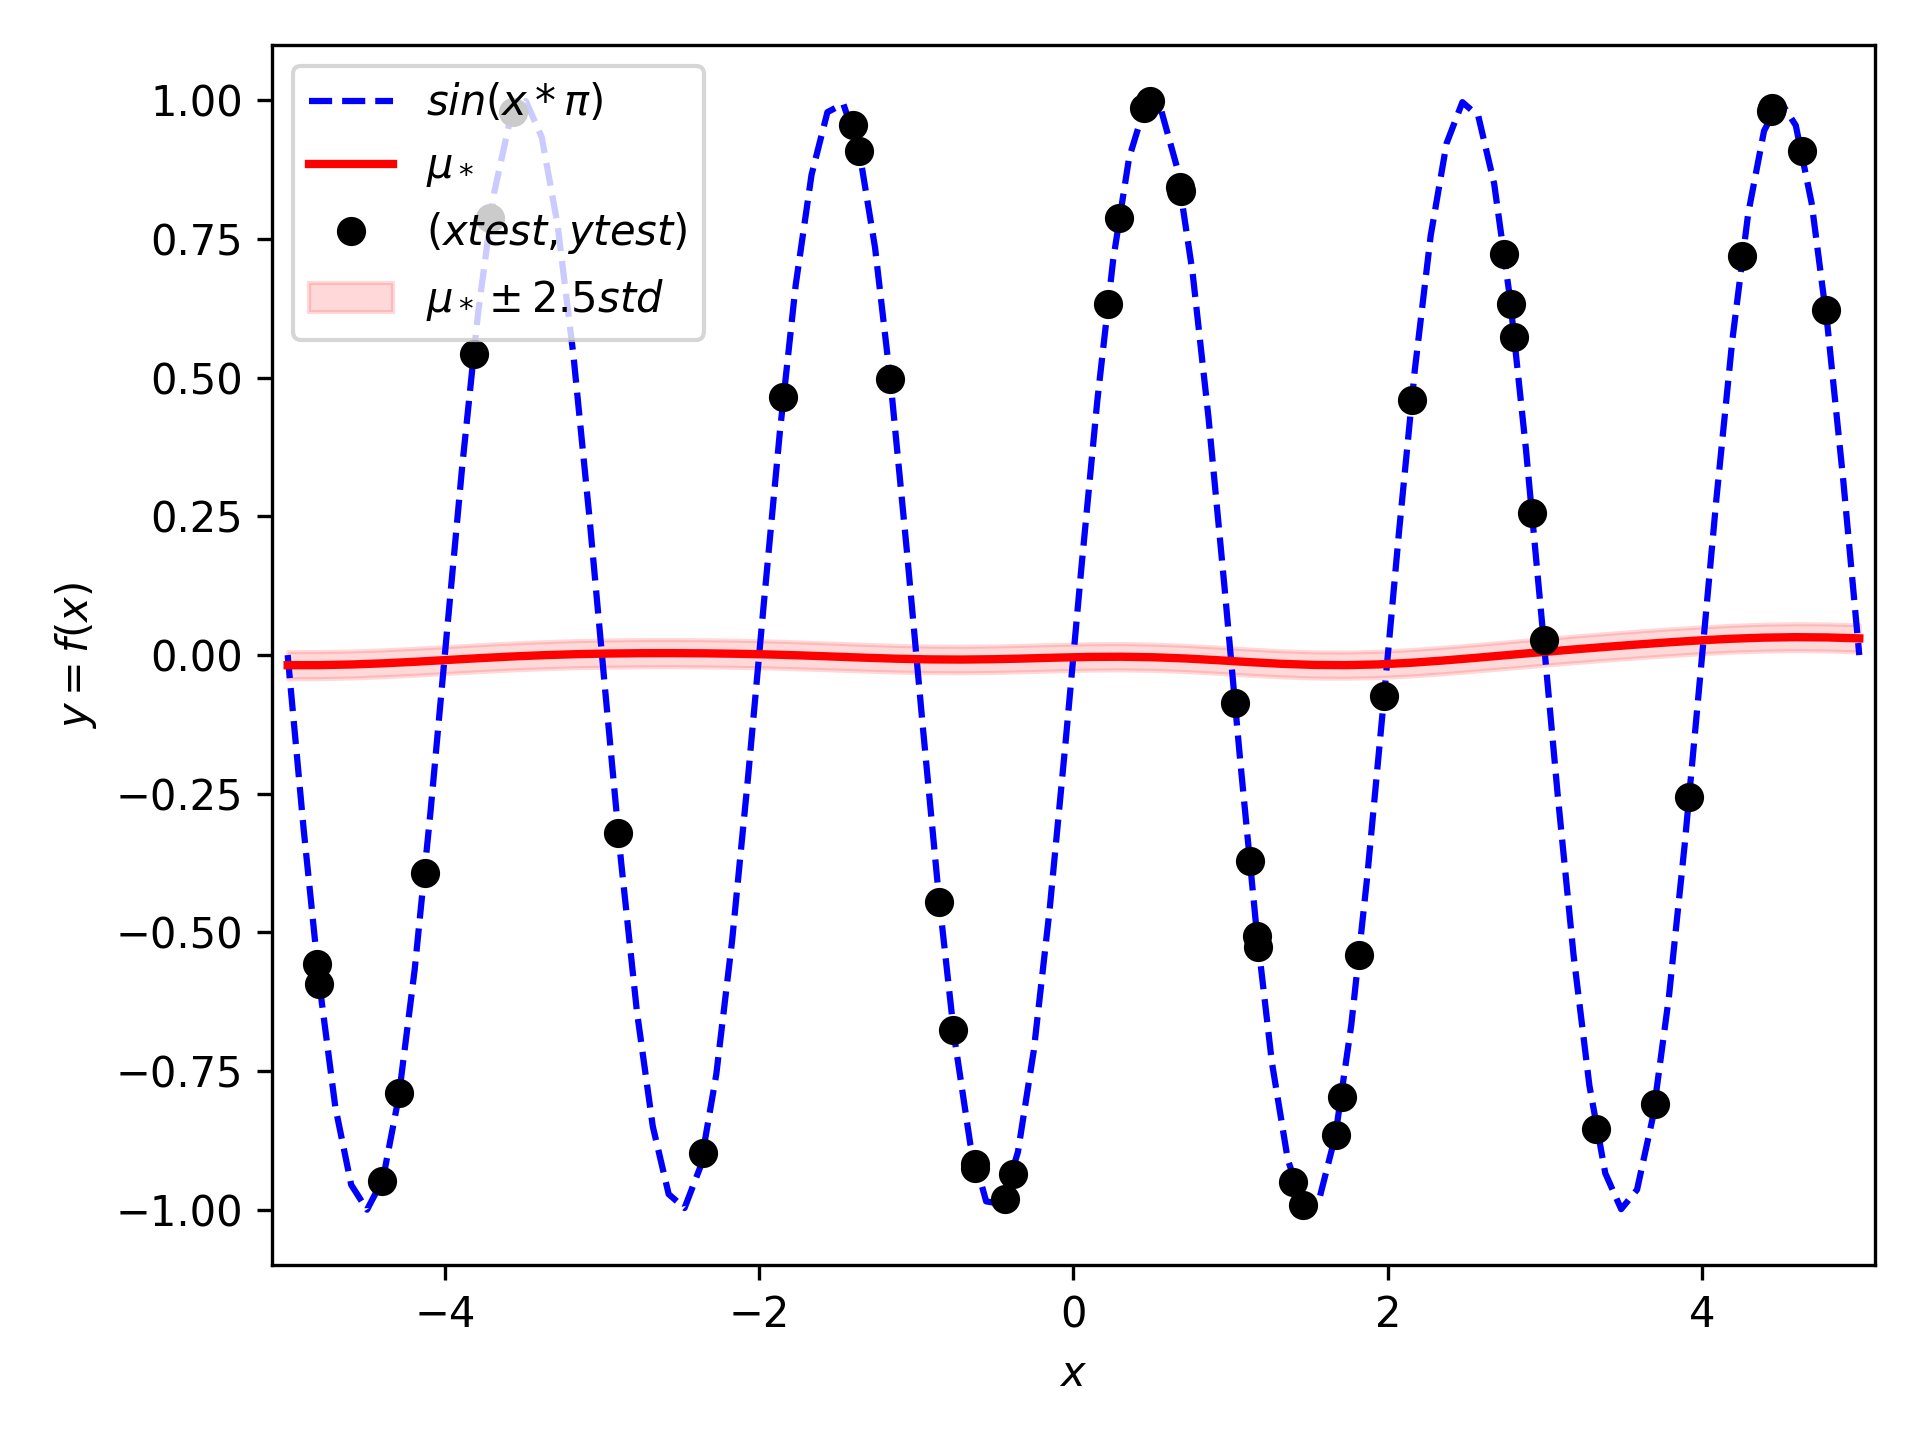
\includegraphics[width=\linewidth]{kernelSE/s/0_01.png}
    \caption{$\sigma = 0.01$}
    \label{fig:s001}
  \end{subfigure}
  \begin{subfigure}{.33\textwidth}
    \centering
    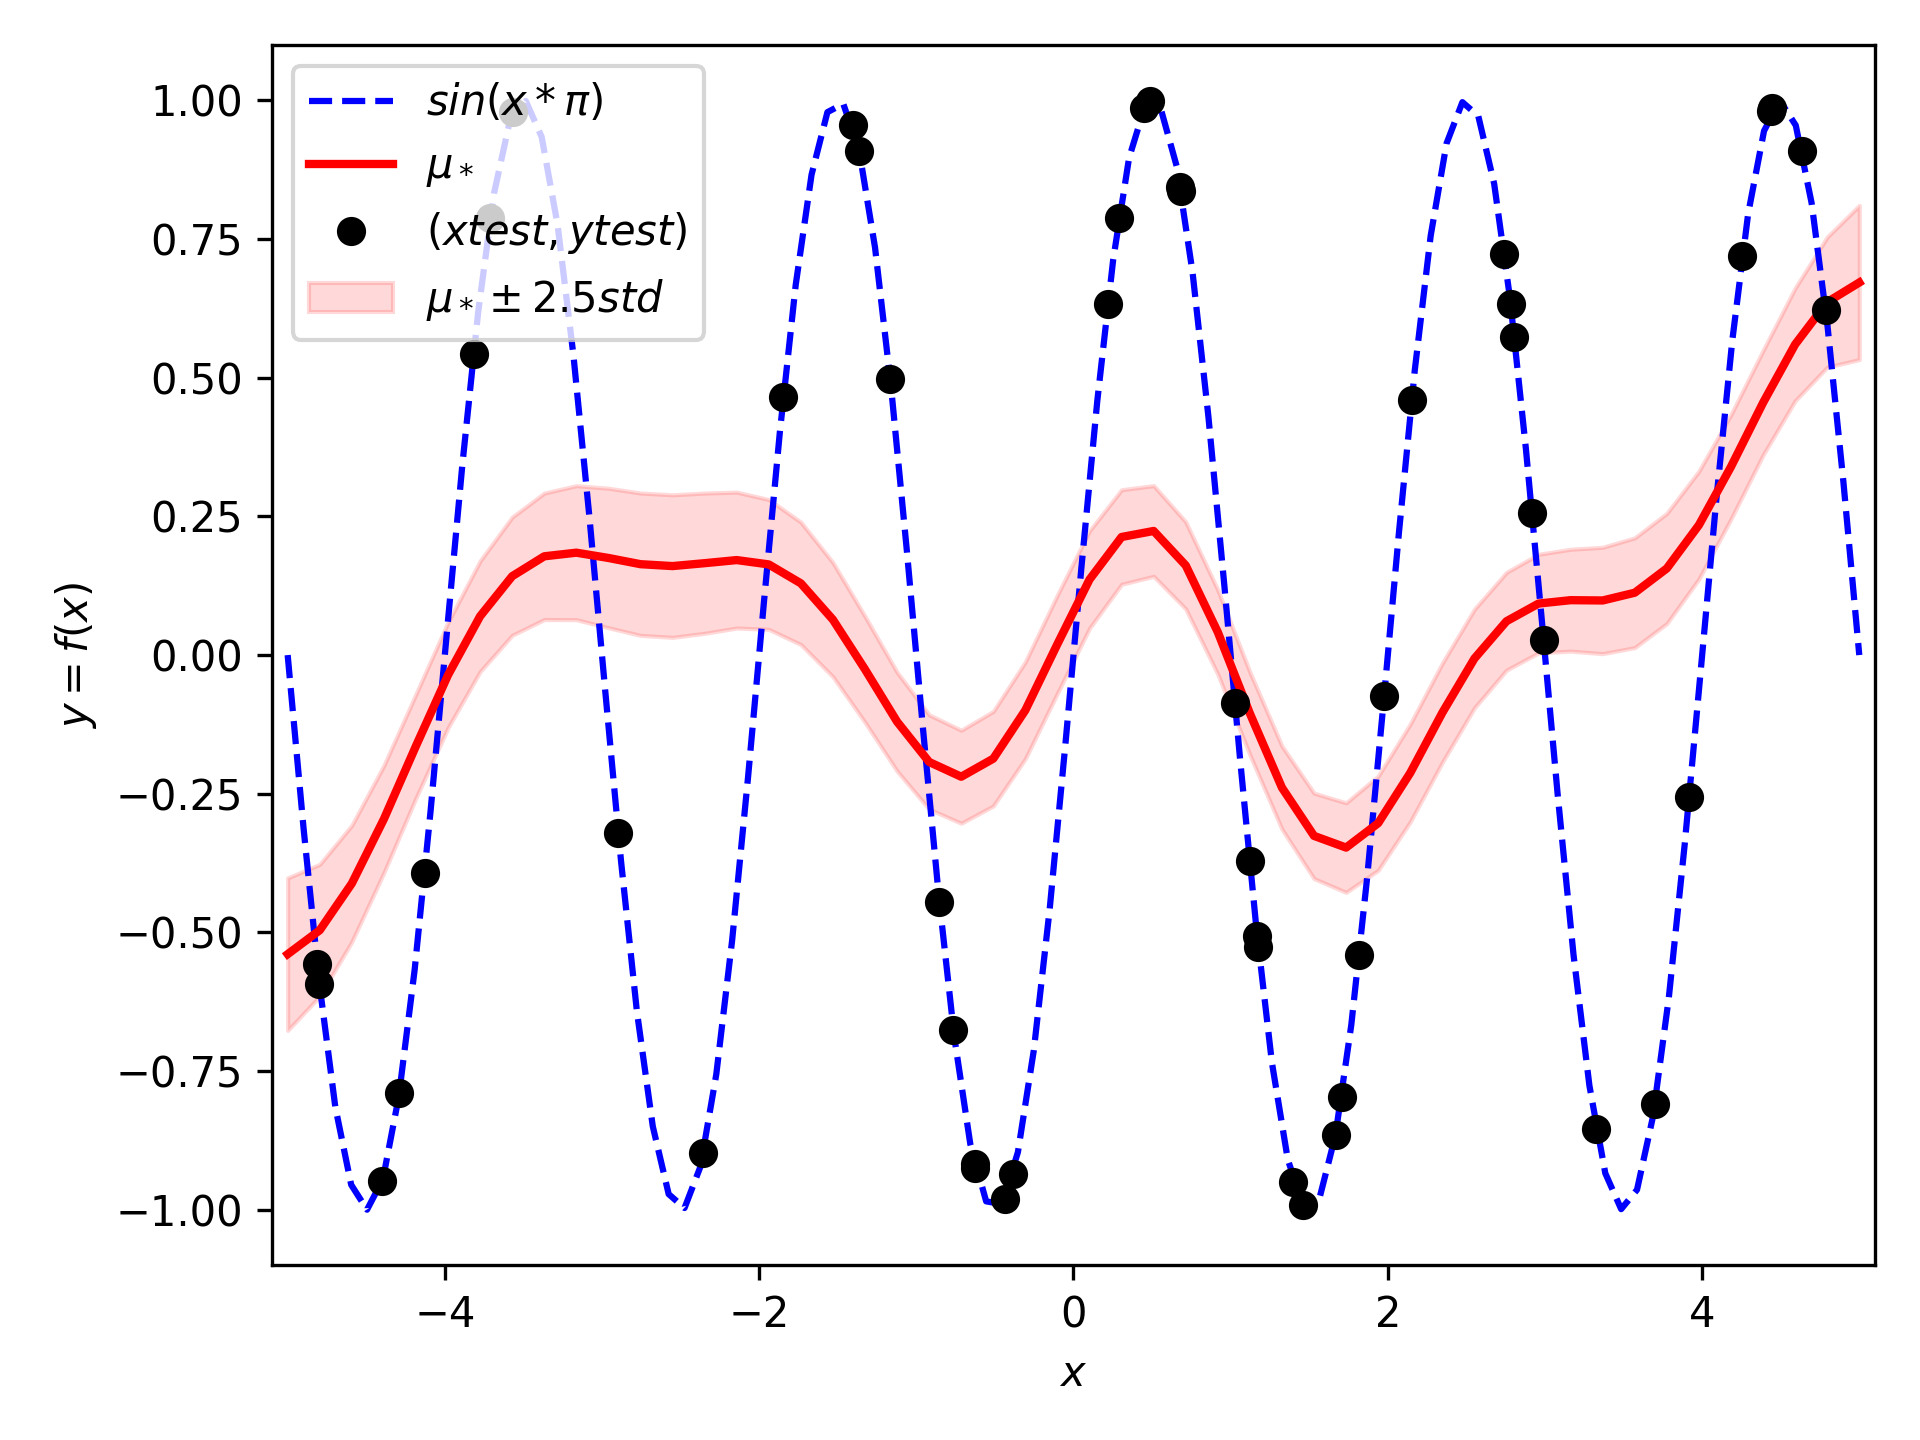
\includegraphics[width=\linewidth]{kernelSE/s/0_1.png}
    \caption{$\sigma = 0.1$}
    \label{fig:s01}
  \end{subfigure}
  \begin{subfigure}{.33\textwidth}
    \centering
    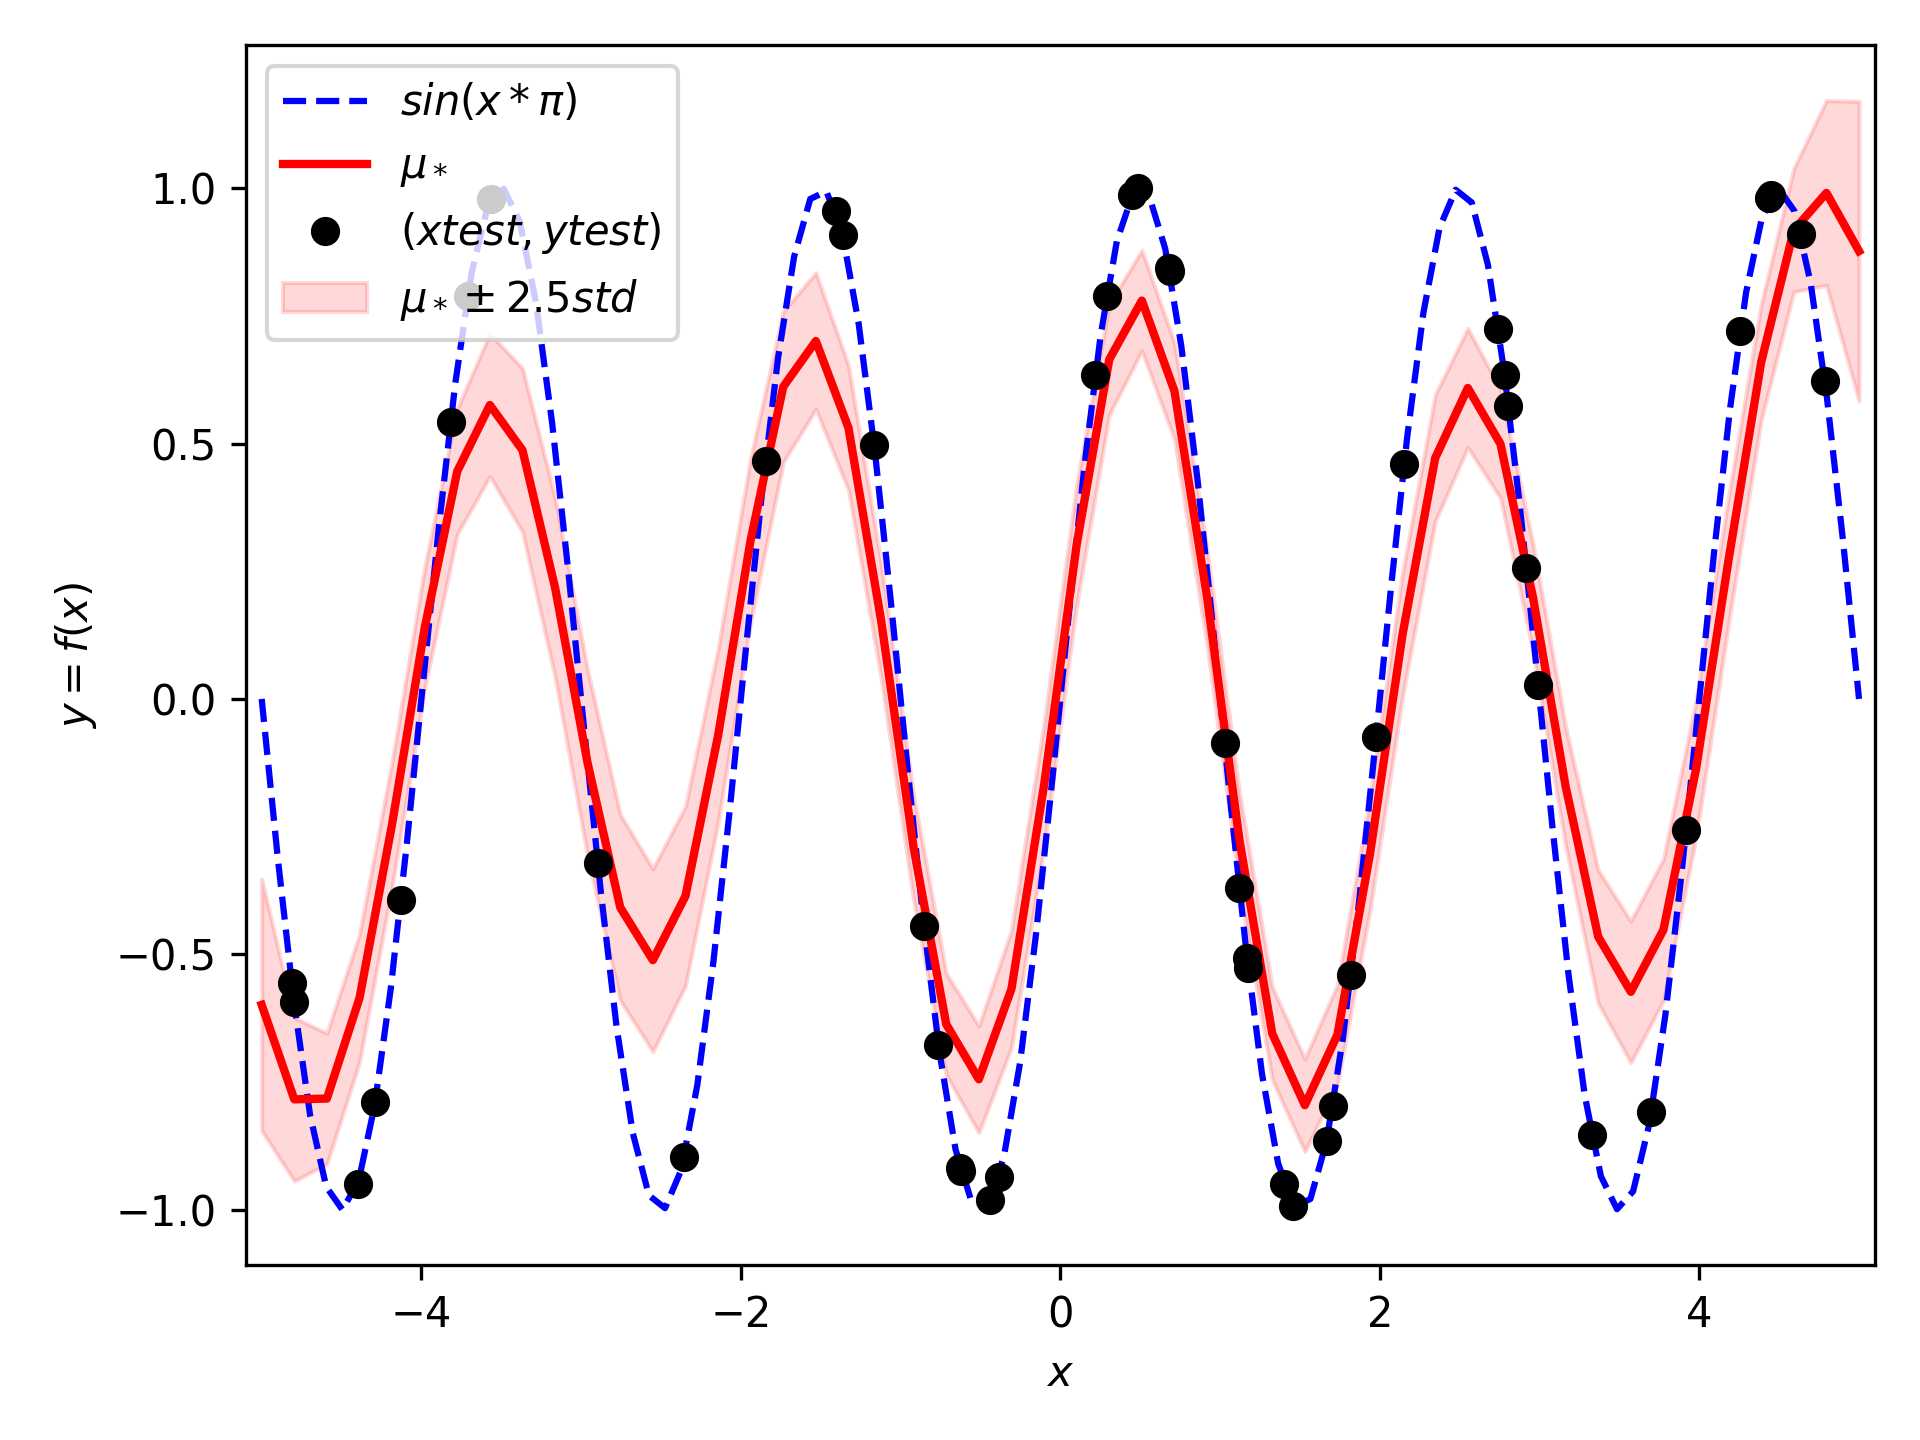
\includegraphics[width=\linewidth]{kernelSE/s/0_5.png}
    \caption{$\sigma = 0.5$}
    \label{fig:s025}
  \end{subfigure}
  \begin{subfigure}{.33\textwidth}
    \centering
    \includegraphics[width=\linewidth]{kernelSE/s/1.png}
    \caption{$\sigma = 1$}
    \label{fig:s05}
  \end{subfigure}
  \begin{subfigure}{.33\textwidth}
    \centering
    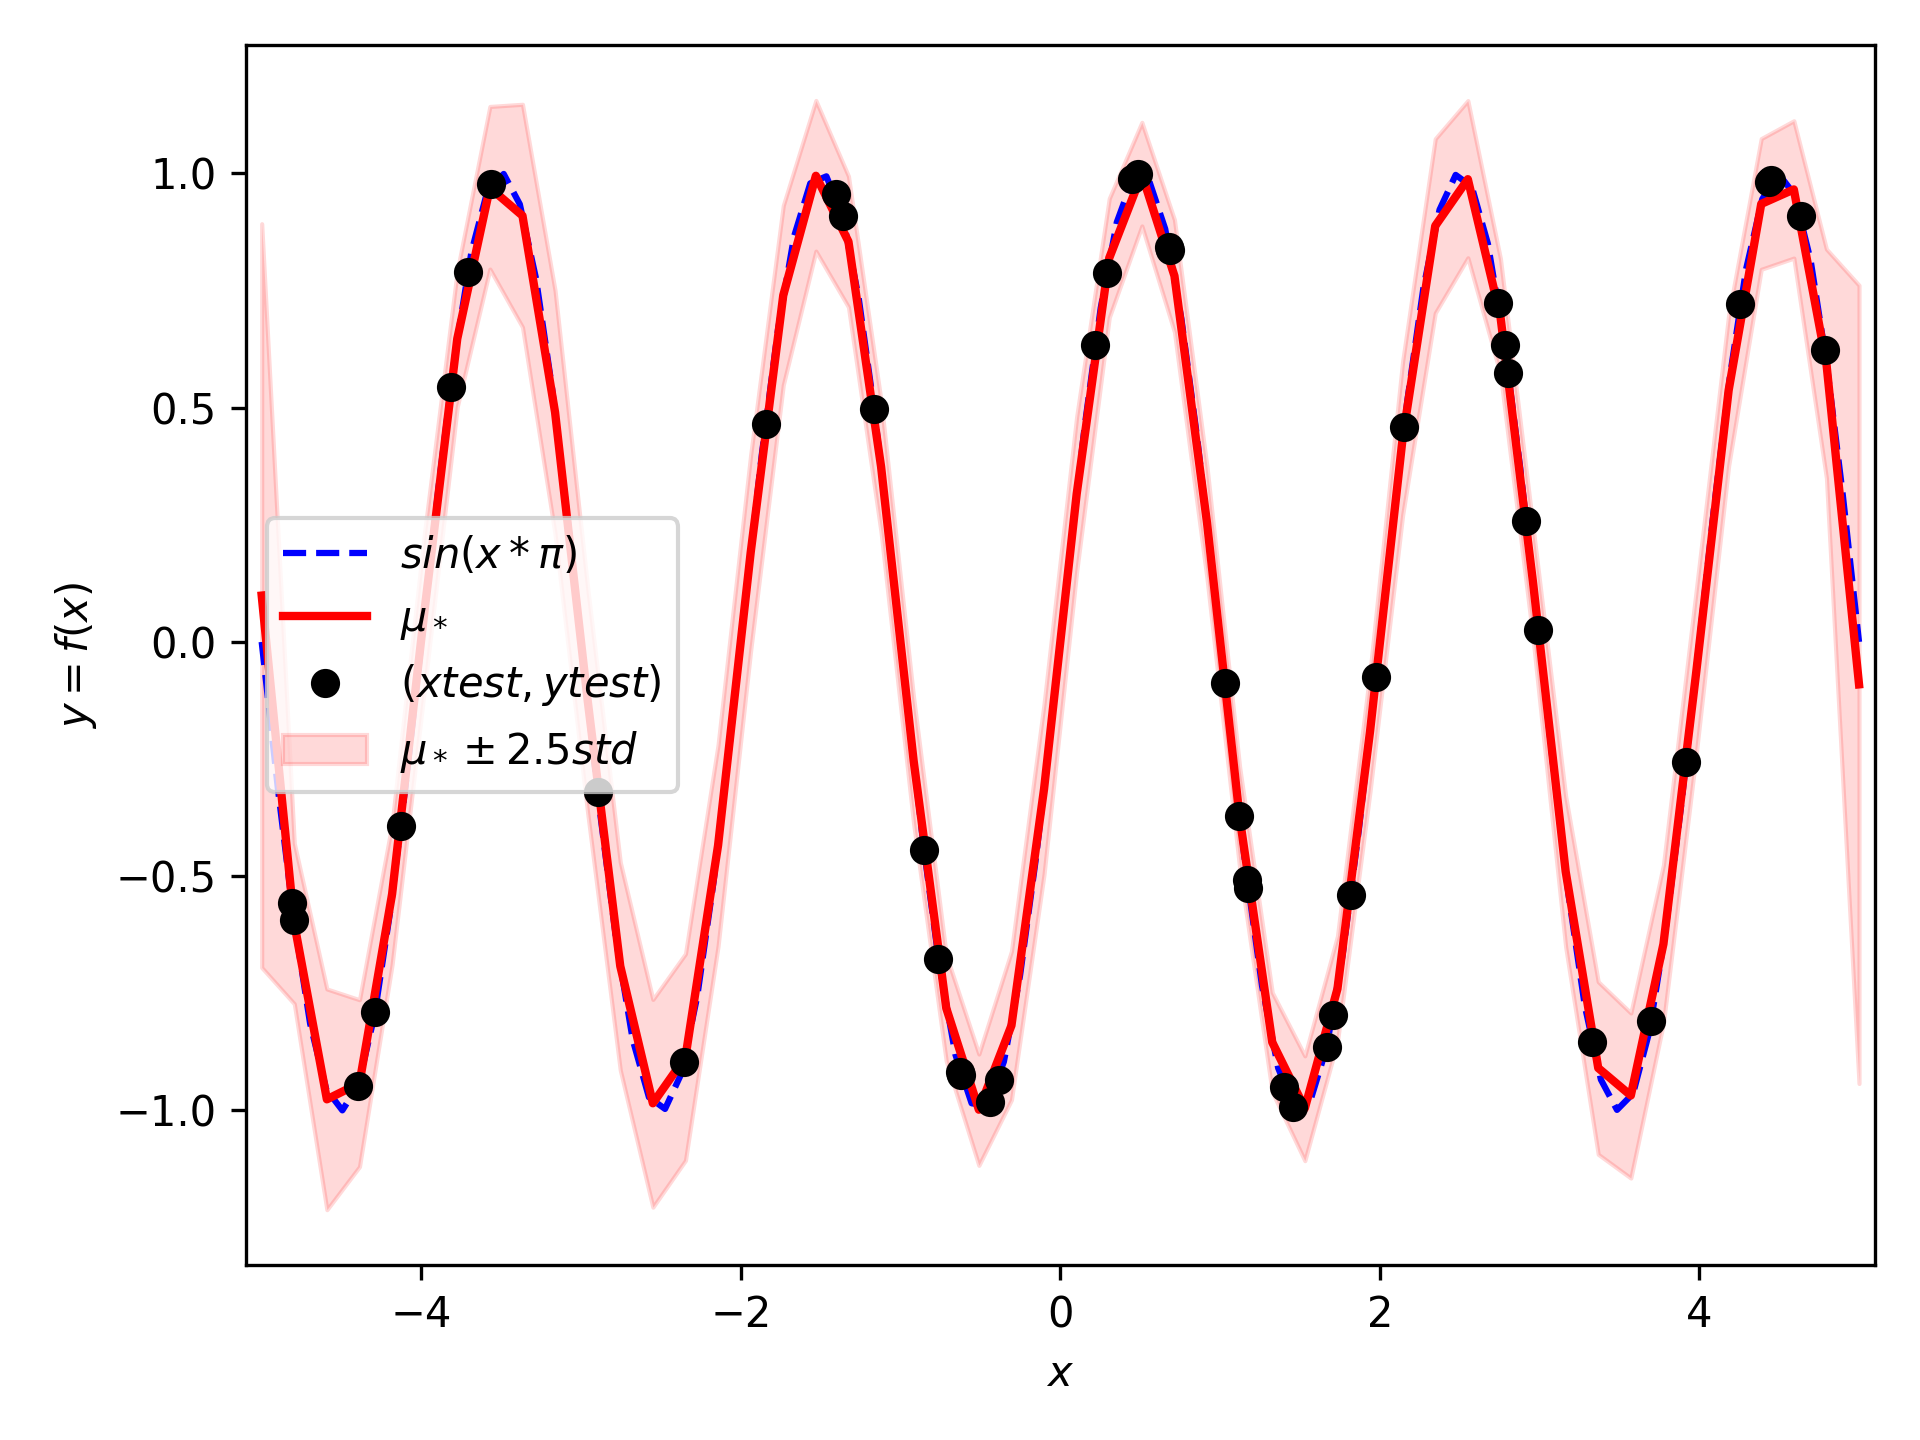
\includegraphics[width=\linewidth]{kernelSE/s/10.png}
    \caption{$\sigma = 10$}
    \label{fig:s075}
  \end{subfigure}
  \begin{subfigure}{.33\textwidth}
    \centering
    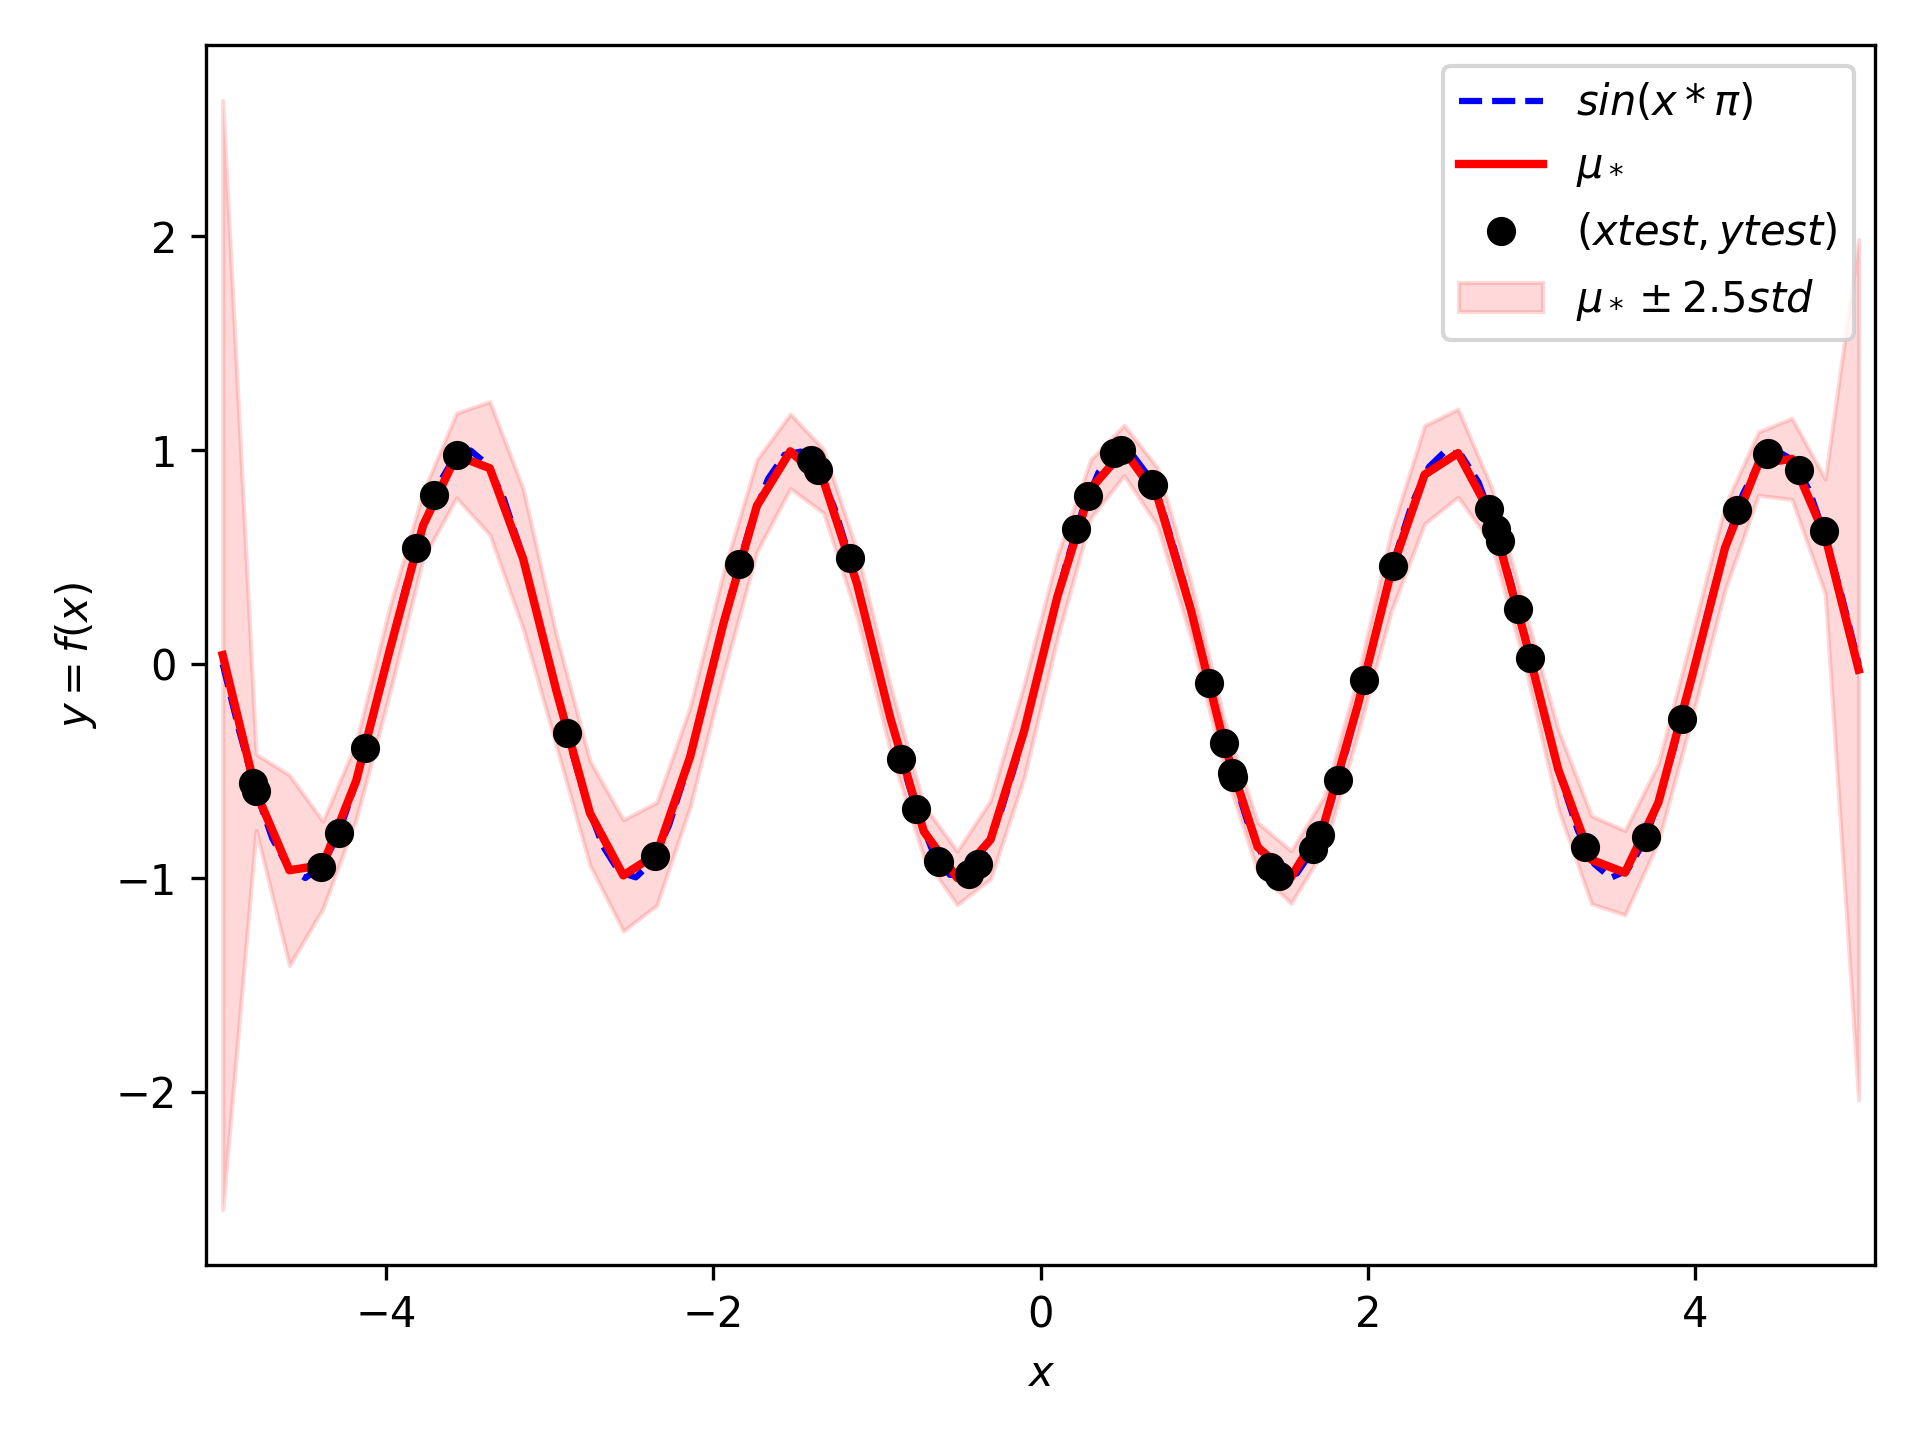
\includegraphics[width=\linewidth]{kernelSE/s/100.png}
    \caption{$\sigma = 100$}
    \label{fig:s1}
  \end{subfigure}
  \caption{Gaussian Processes with SE kernel with different values of $\sigma$. The remaining parameters of SE kernel are fixed ($\ell = 1$ and $\sigma_y^2 = 0.01$).}
  \label{fig:sigma}
\end{figure}

\subsubsection{Parameters $\sigma_y^2$}

We evaluated effects of the parameters $\sigma_y^2$ on our predictions, keeping the remaing parameters ($\ell$ and $\sigma$) in their default value (Fig. \ref{fig:noise}).

As observed in Fig. \ref{fig:noise}, when the noise is small, the curve has a good fit to our target function and the uncertainty becomes really small (\ie small confidence interval). As the noise increase, the curve becomes smoother, until it becomes a straight line, and, at the same time, the uncertainty increases (\ie wider confidence interval). Therefore, the ideal scenario is to make observations with as little noise as possible for the best results.

% noise
\begin{figure}[ht]
  \begin{subfigure}{.33\textwidth}
    \centering
    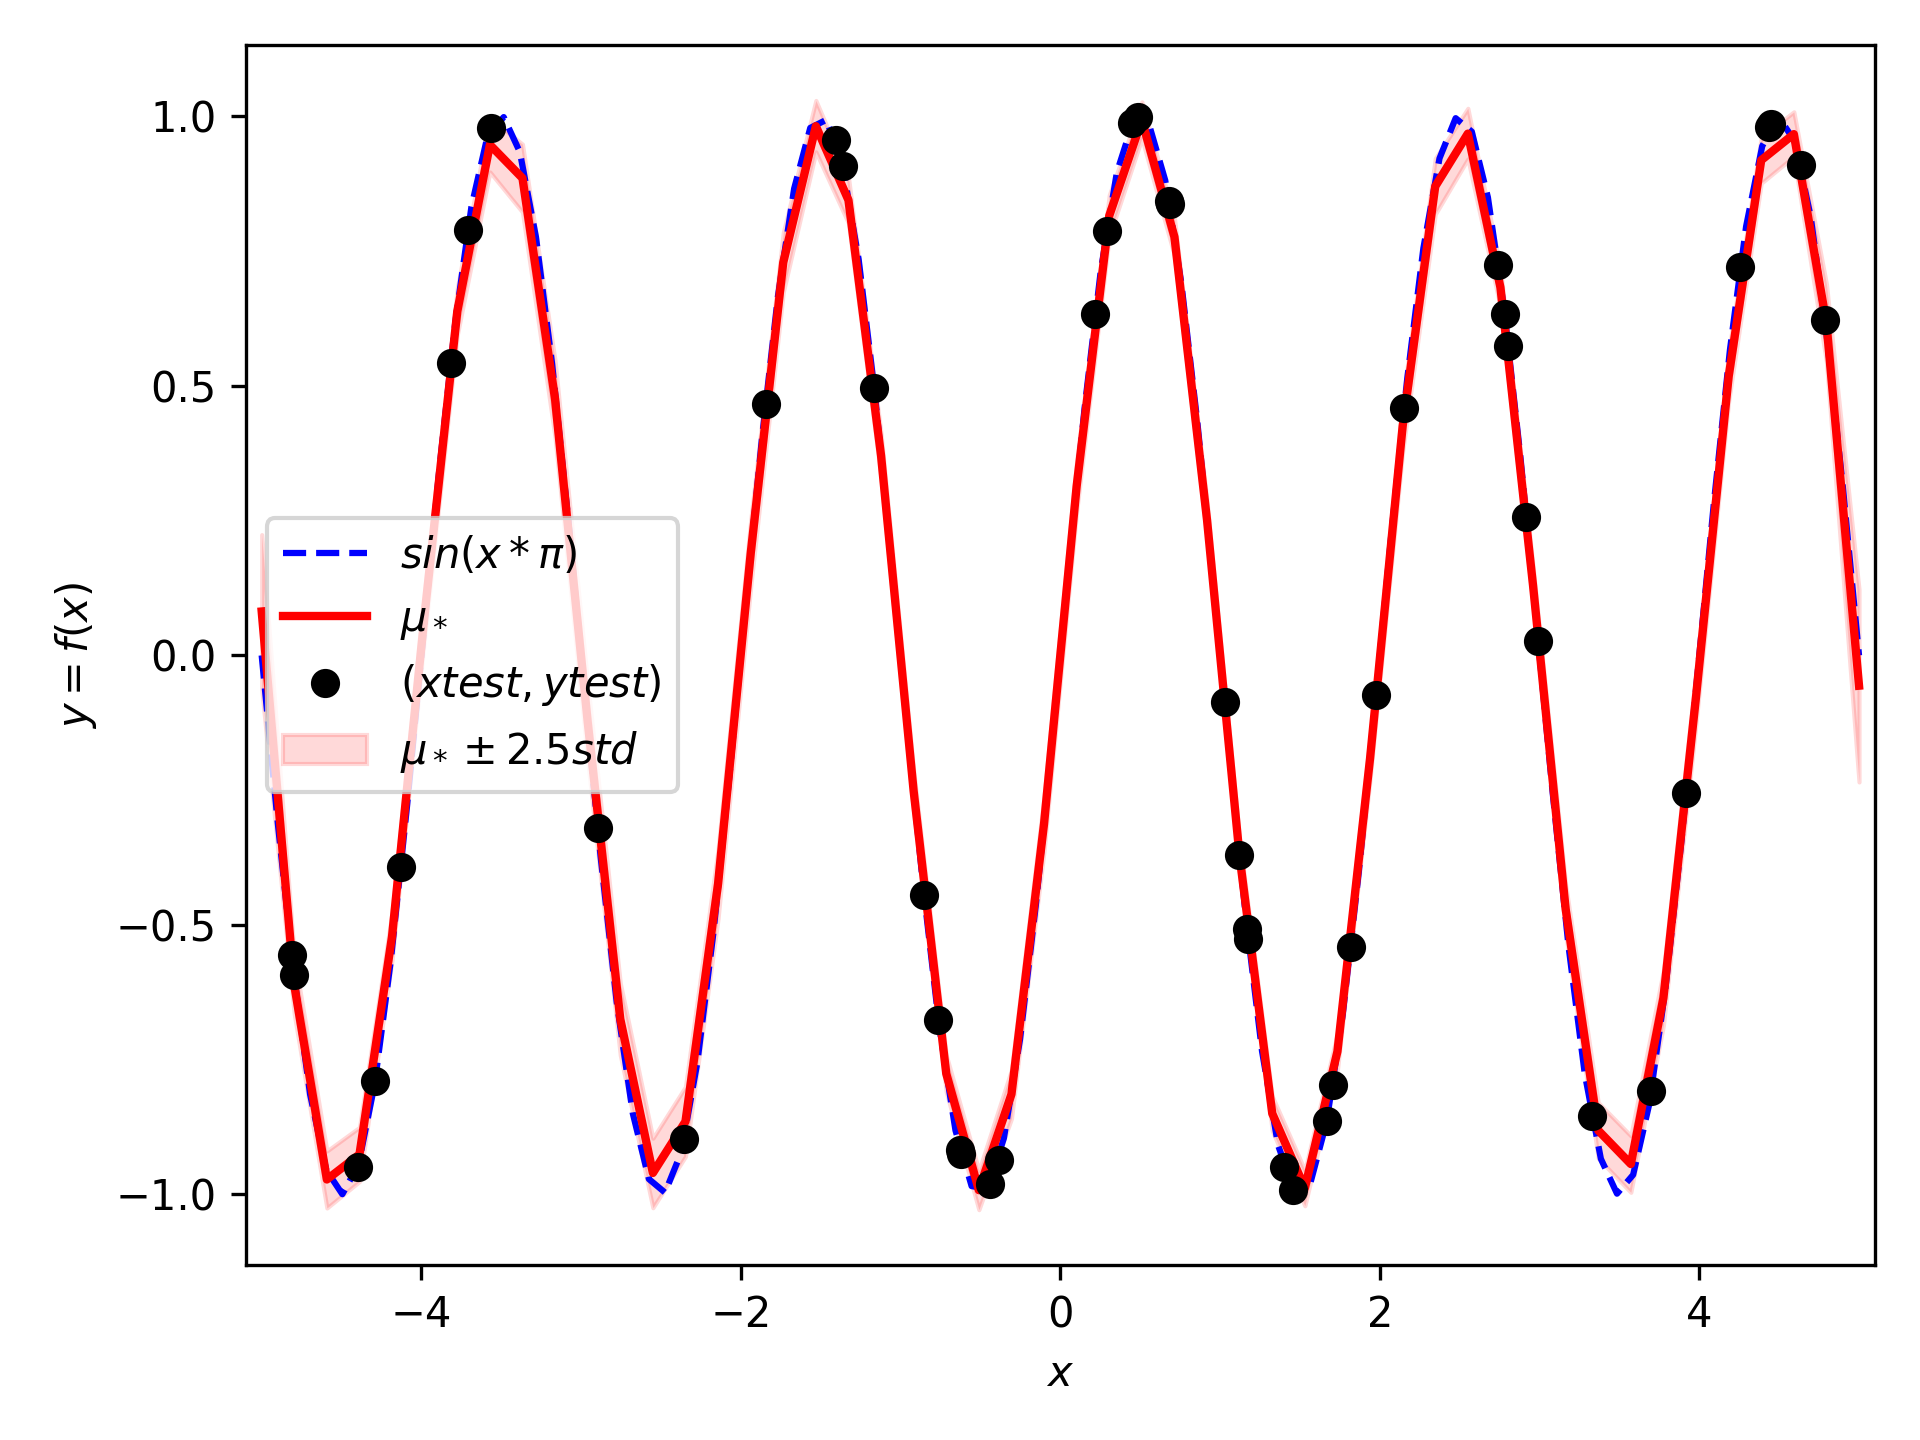
\includegraphics[width=\linewidth]{kernelSE/noise/0_001.png}
    \caption{$\sigma_y^2 = 0.001$}
    \label{fig:noise0001}
  \end{subfigure}
  \begin{subfigure}{.33\textwidth}
    \centering
    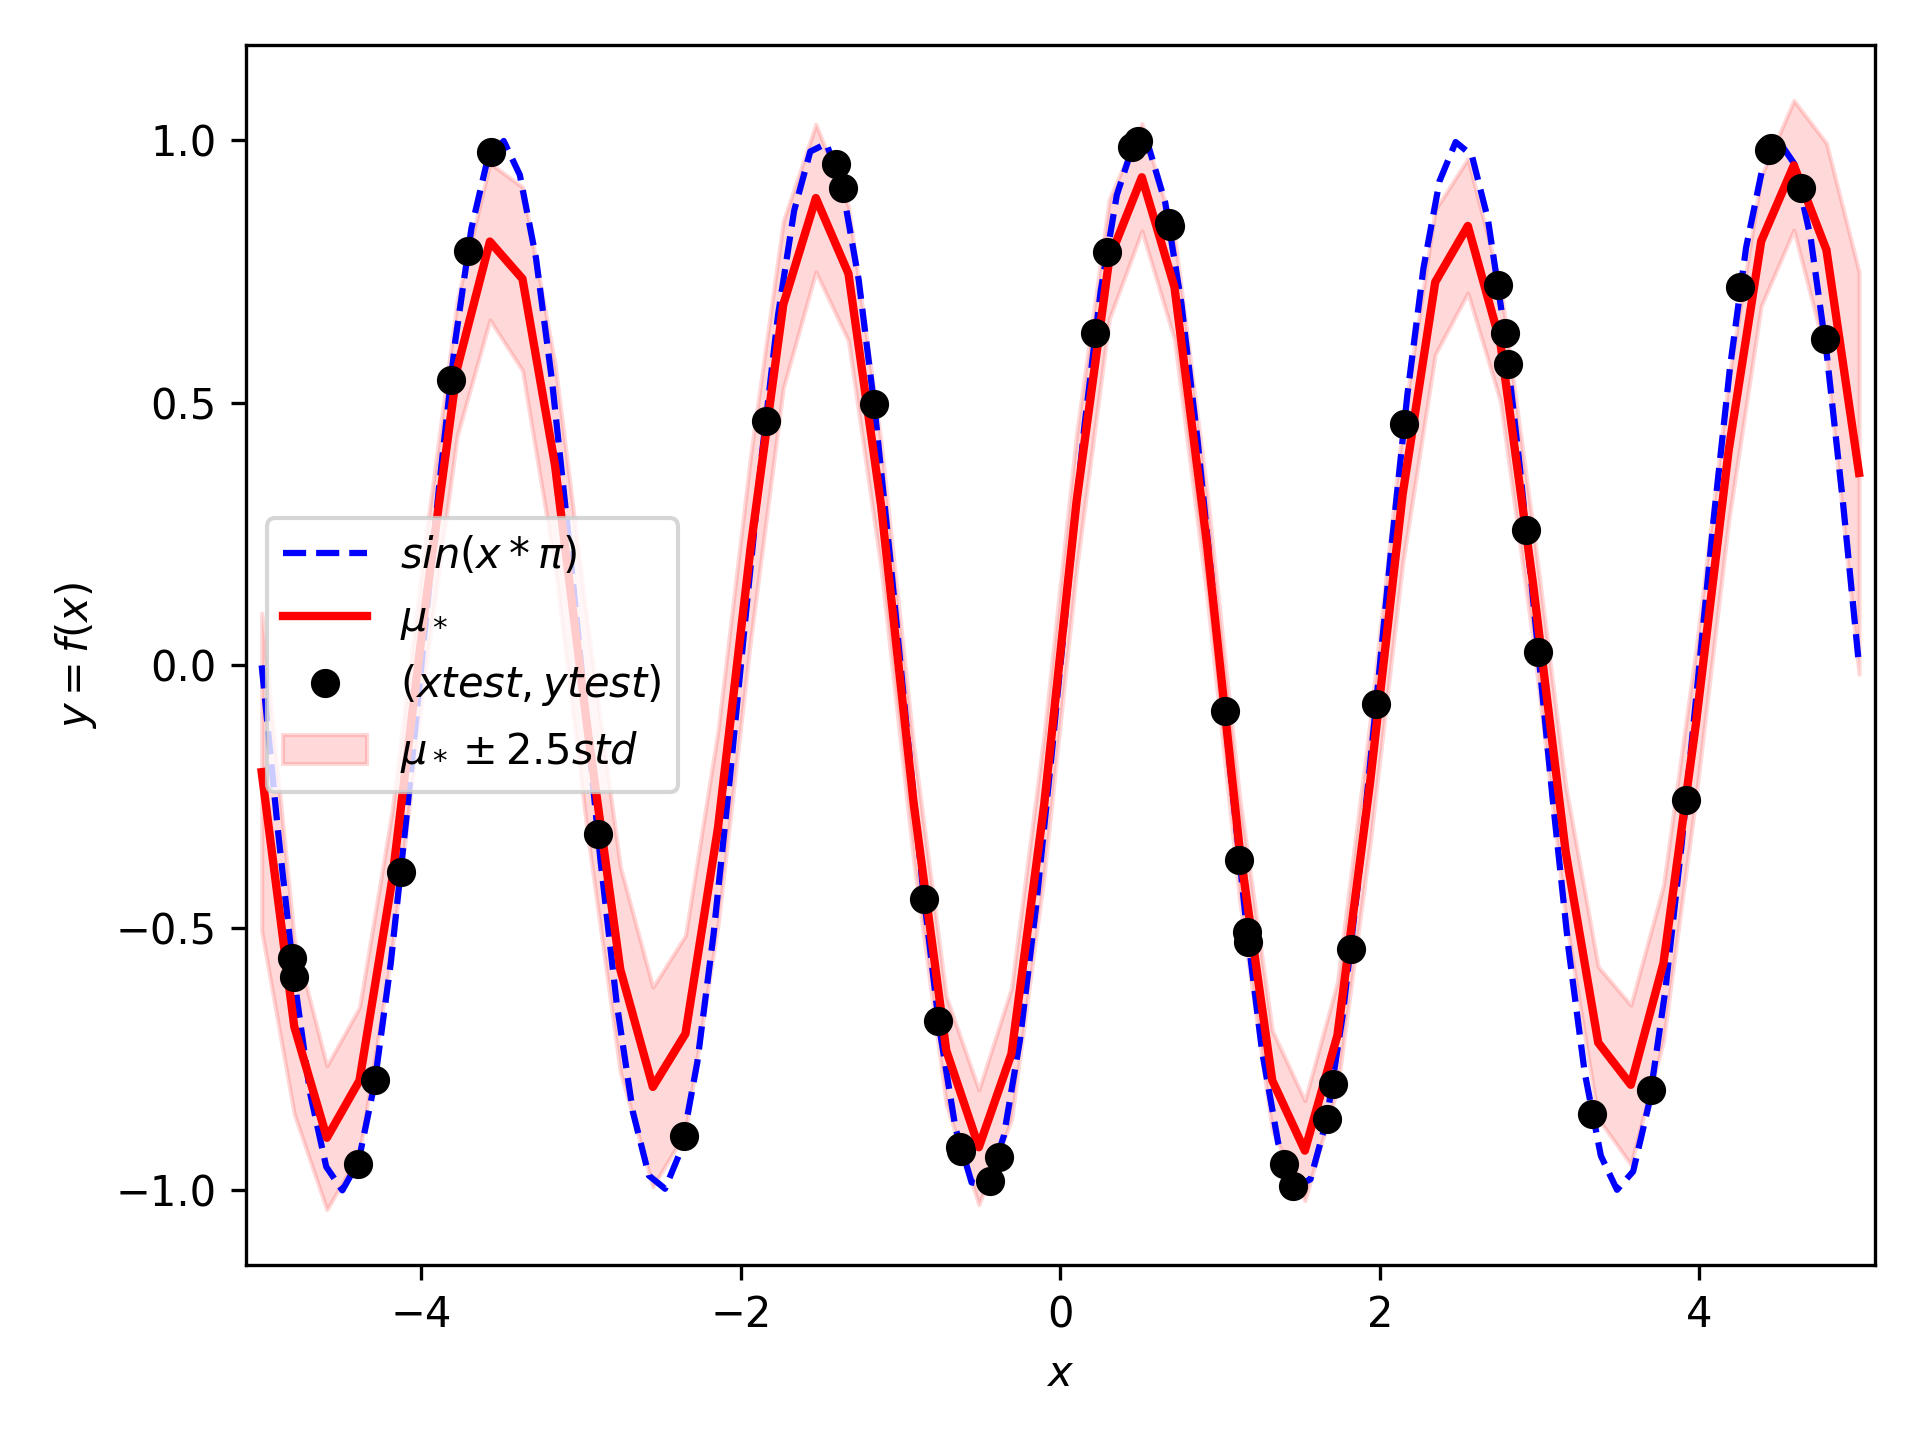
\includegraphics[width=\linewidth]{kernelSE/noise/0_01.png}
    \caption{$\sigma_y^2 = 0.01$}
    \label{fig:noise001}
  \end{subfigure}
  \begin{subfigure}{.33\textwidth}
    \centering
    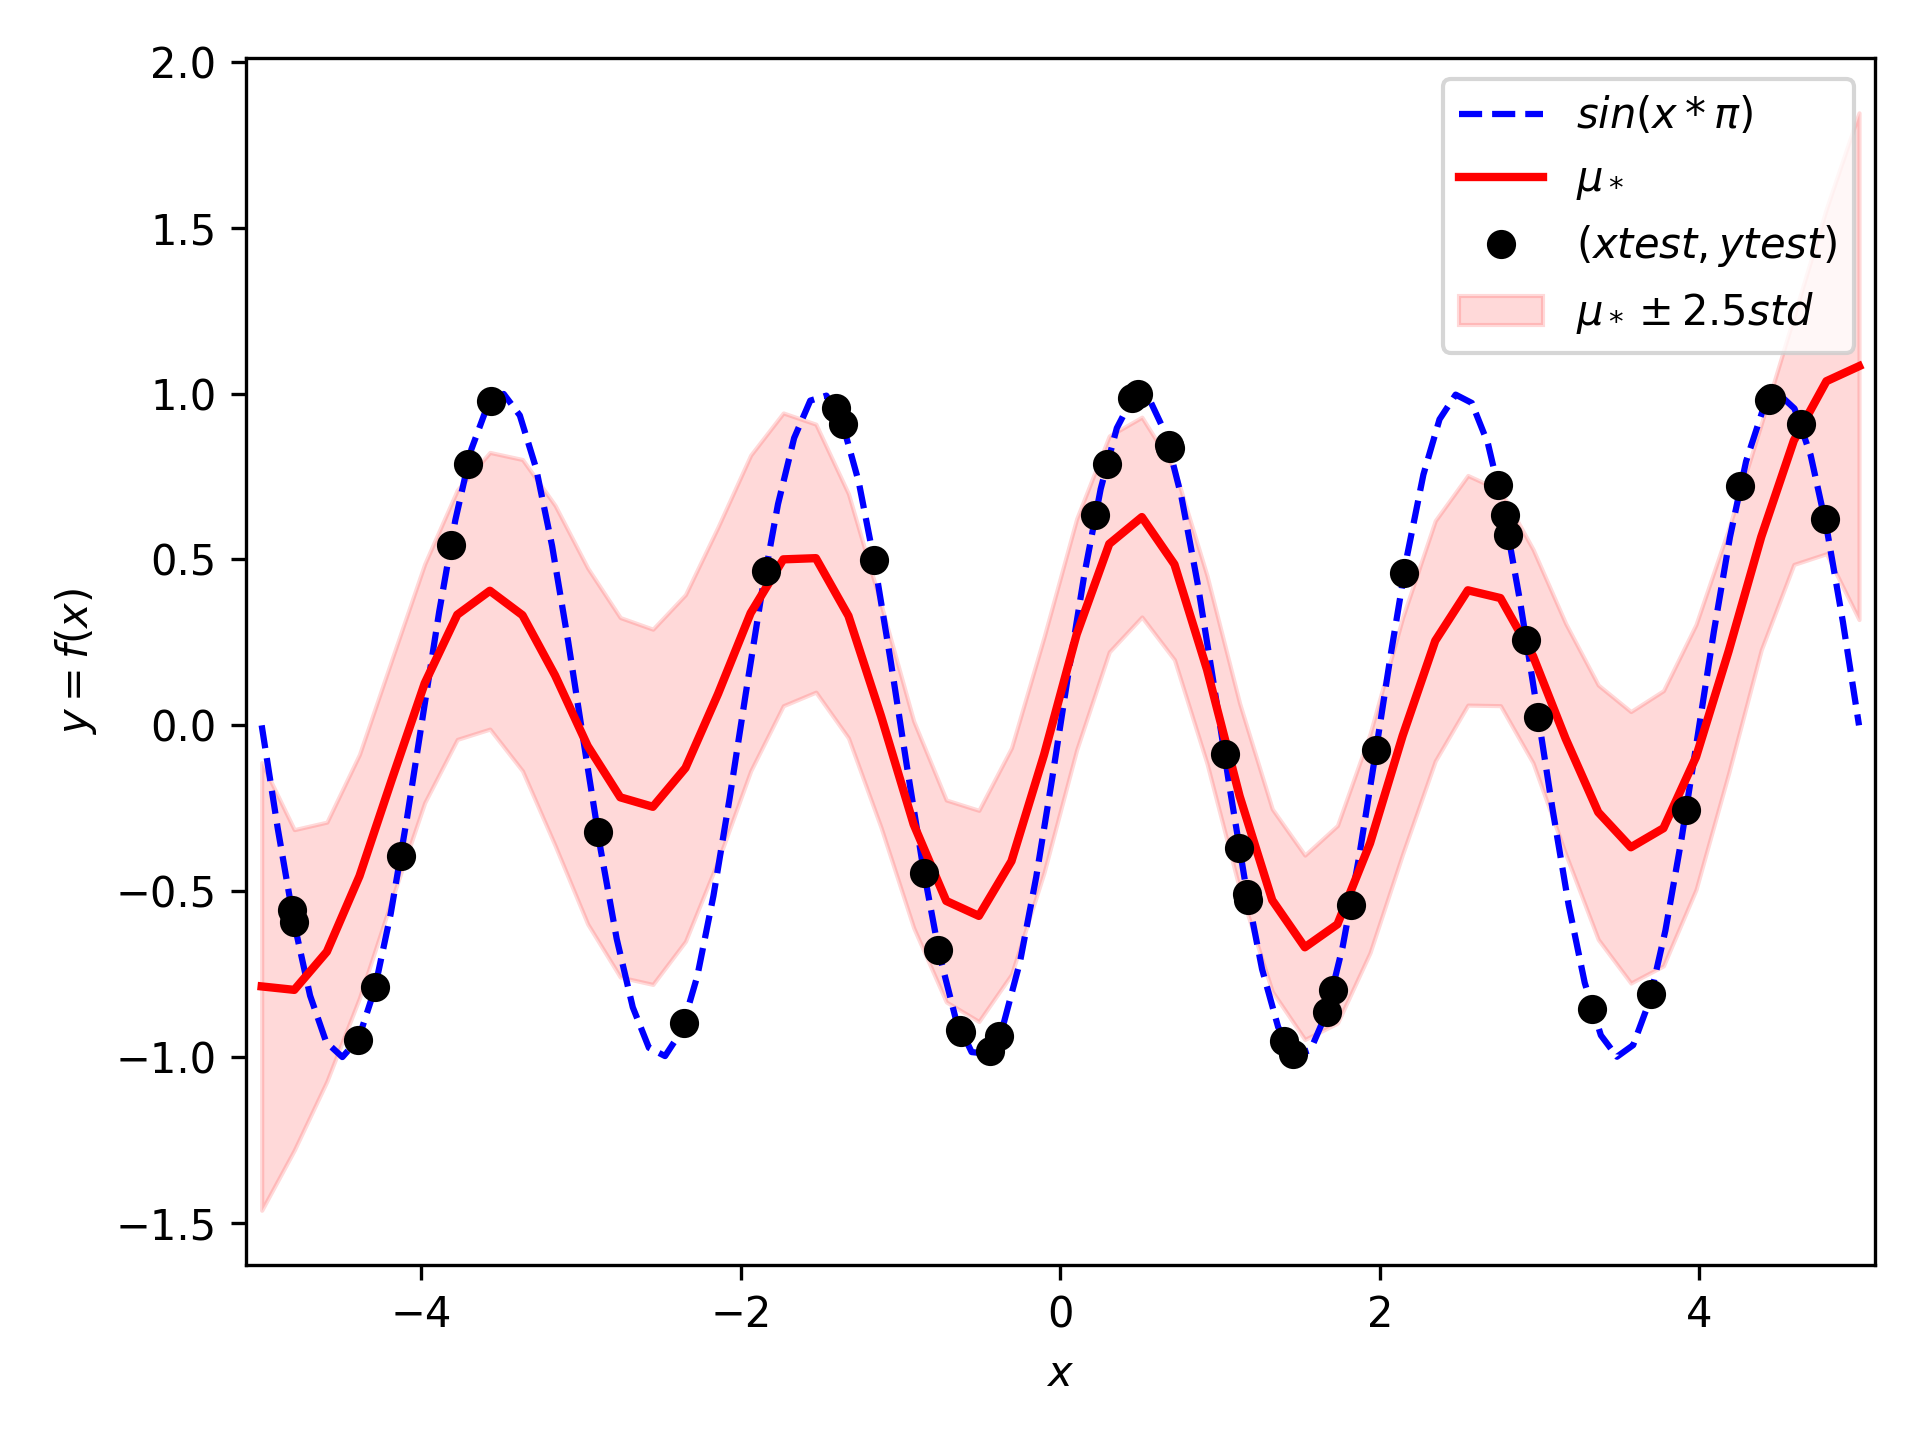
\includegraphics[width=\linewidth]{kernelSE/noise/0_1.png}
    \caption{$\sigma_y^2 = 0.1$}
    \label{fig:noise01}
  \end{subfigure}
  \begin{subfigure}{.33\textwidth}
    \centering
    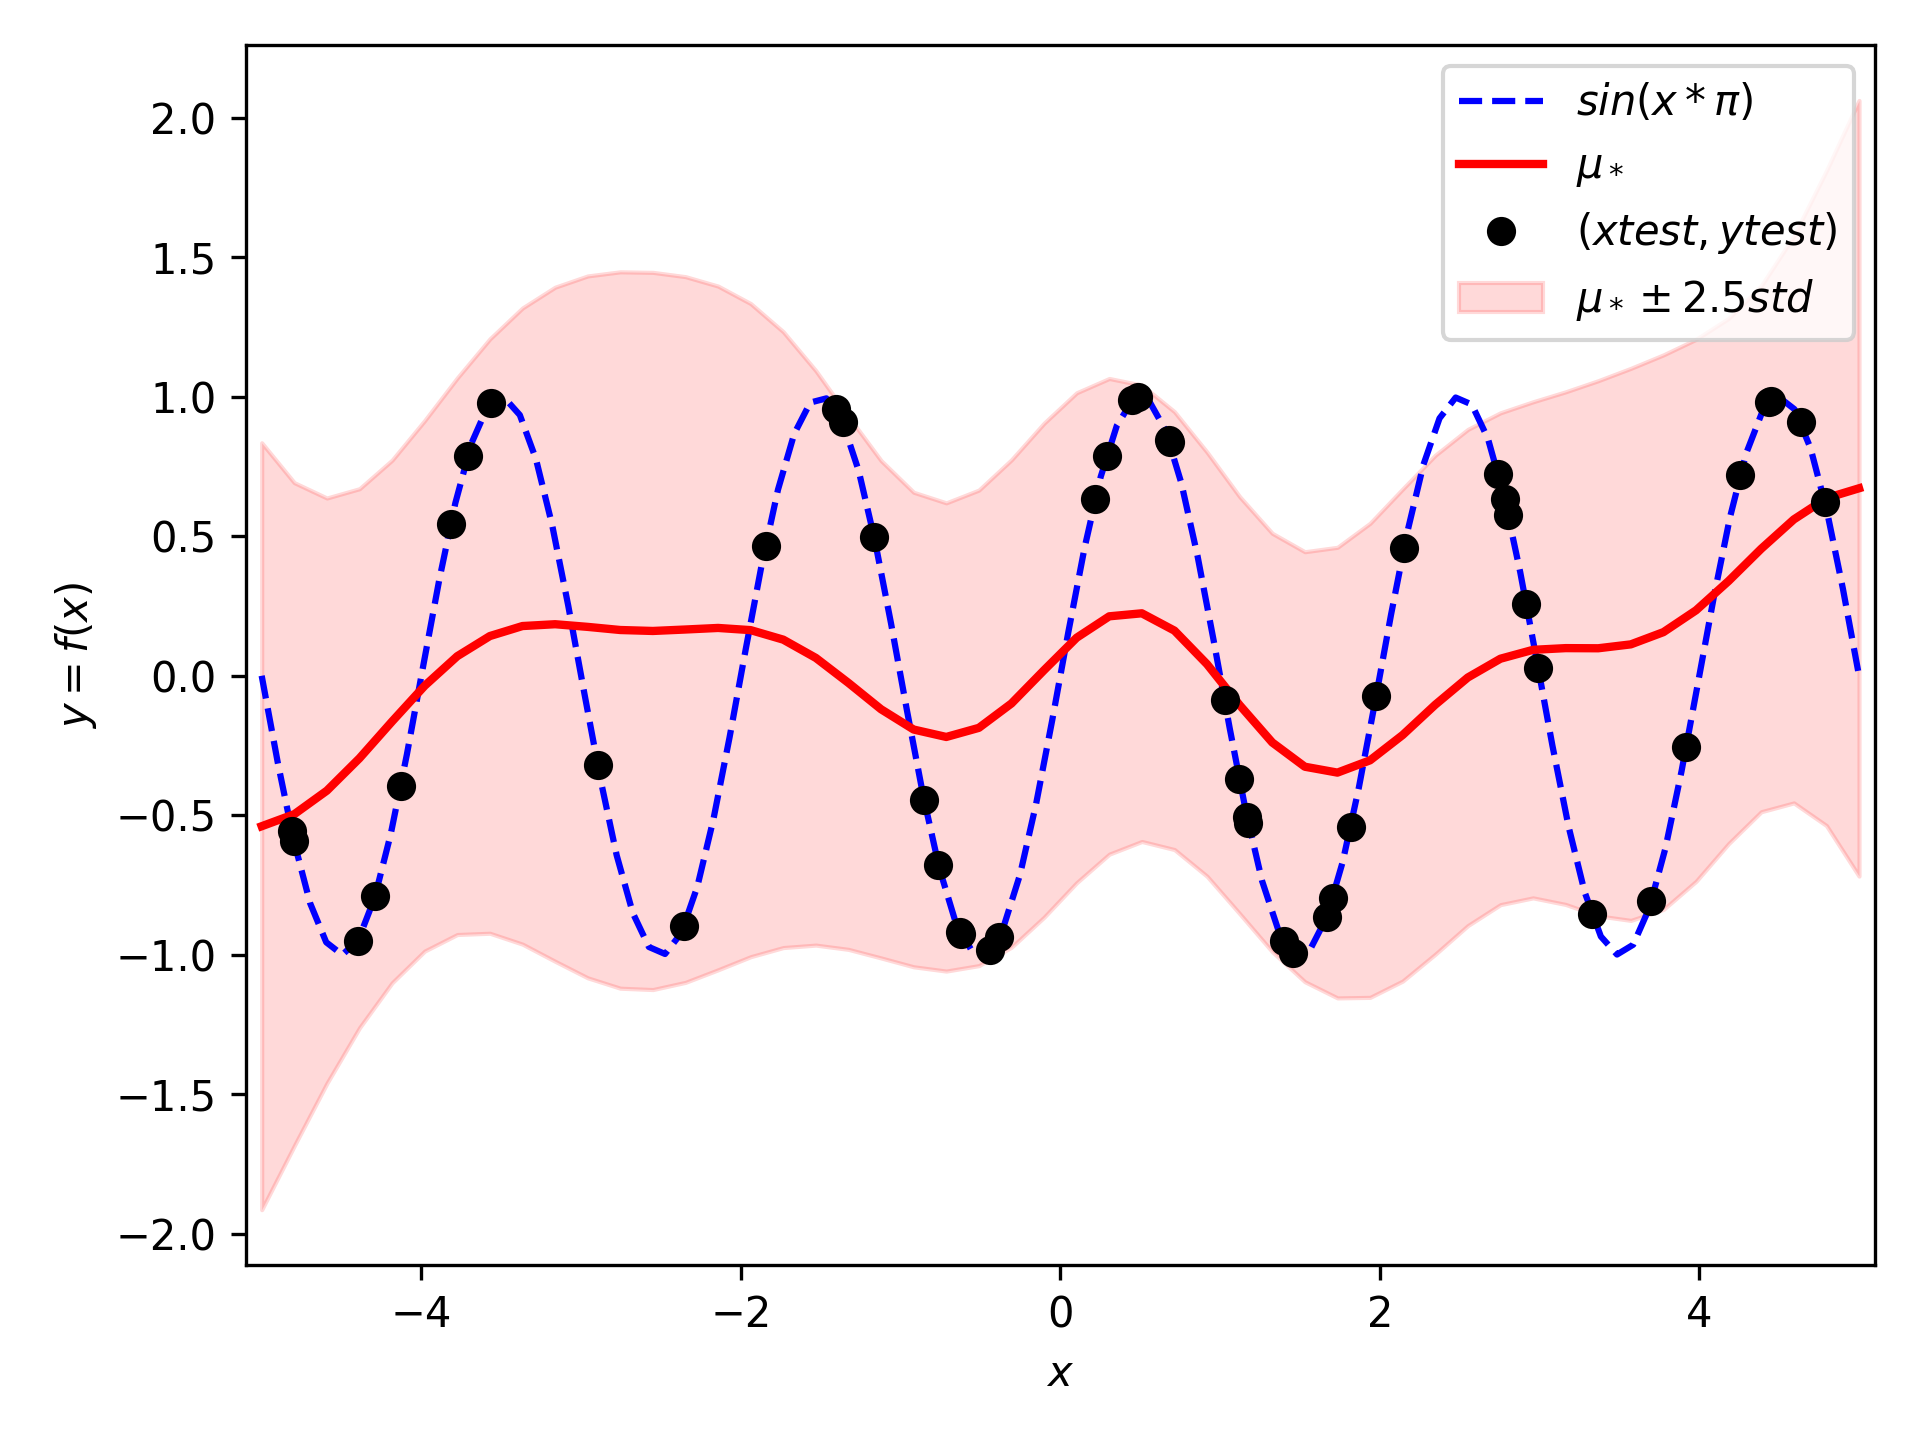
\includegraphics[width=\linewidth]{kernelSE/noise/1.png}
    \caption{$\sigma_y^2 = 1$}
    \label{fig:noise1}
  \end{subfigure}
  \begin{subfigure}{.33\textwidth}
    \centering
    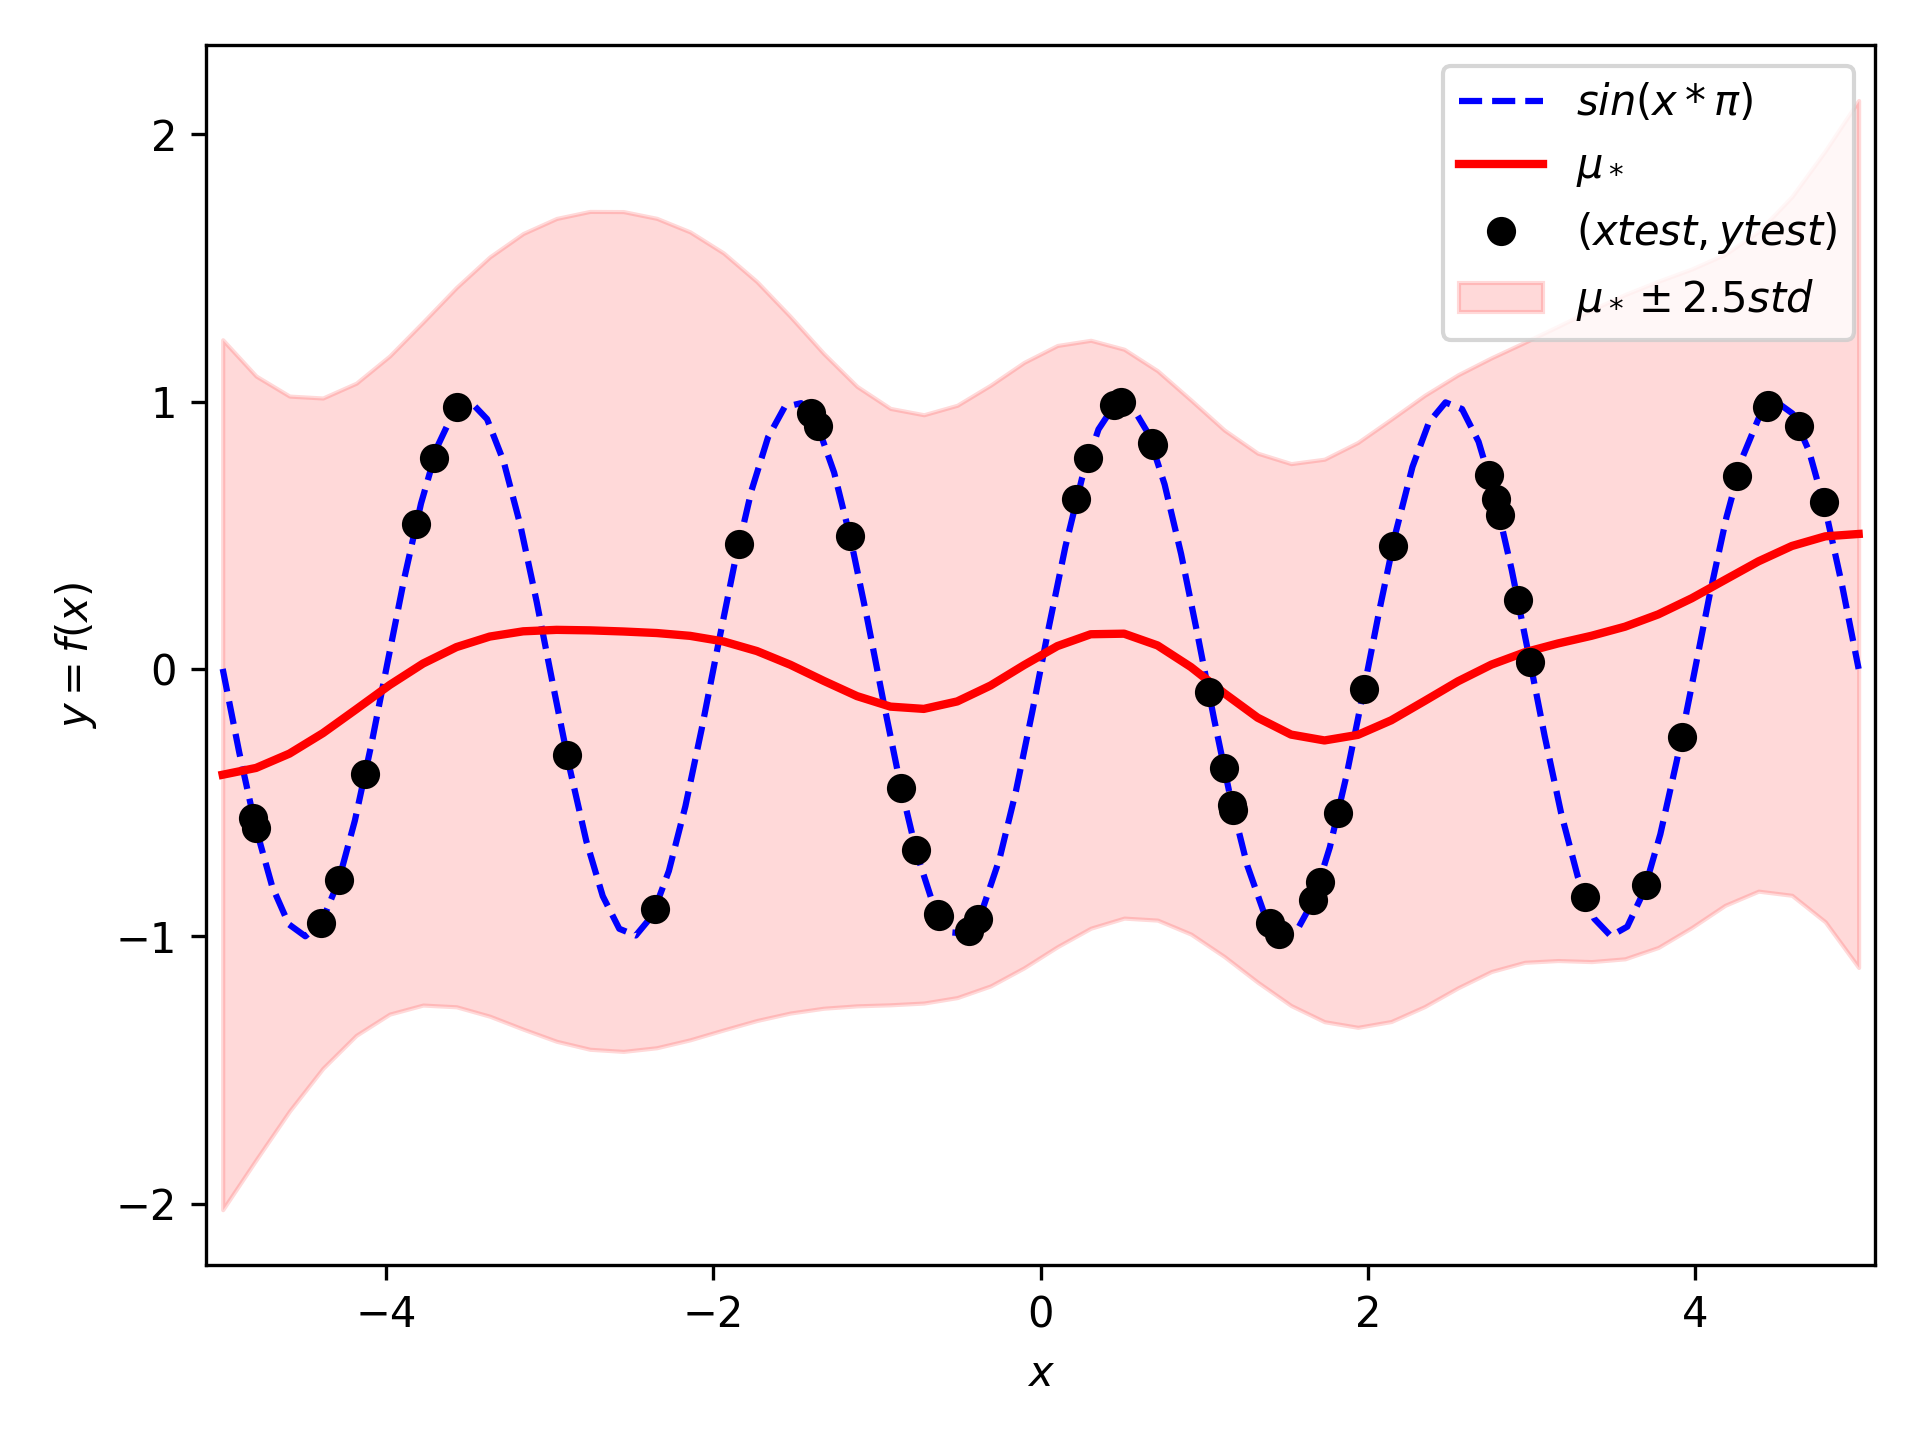
\includegraphics[width=\linewidth]{kernelSE/noise/2.png}
    \caption{$\sigma_y^2 = 2$}
    \label{fig:noise2}
  \end{subfigure}
  \begin{subfigure}{.33\textwidth}
    \centering
    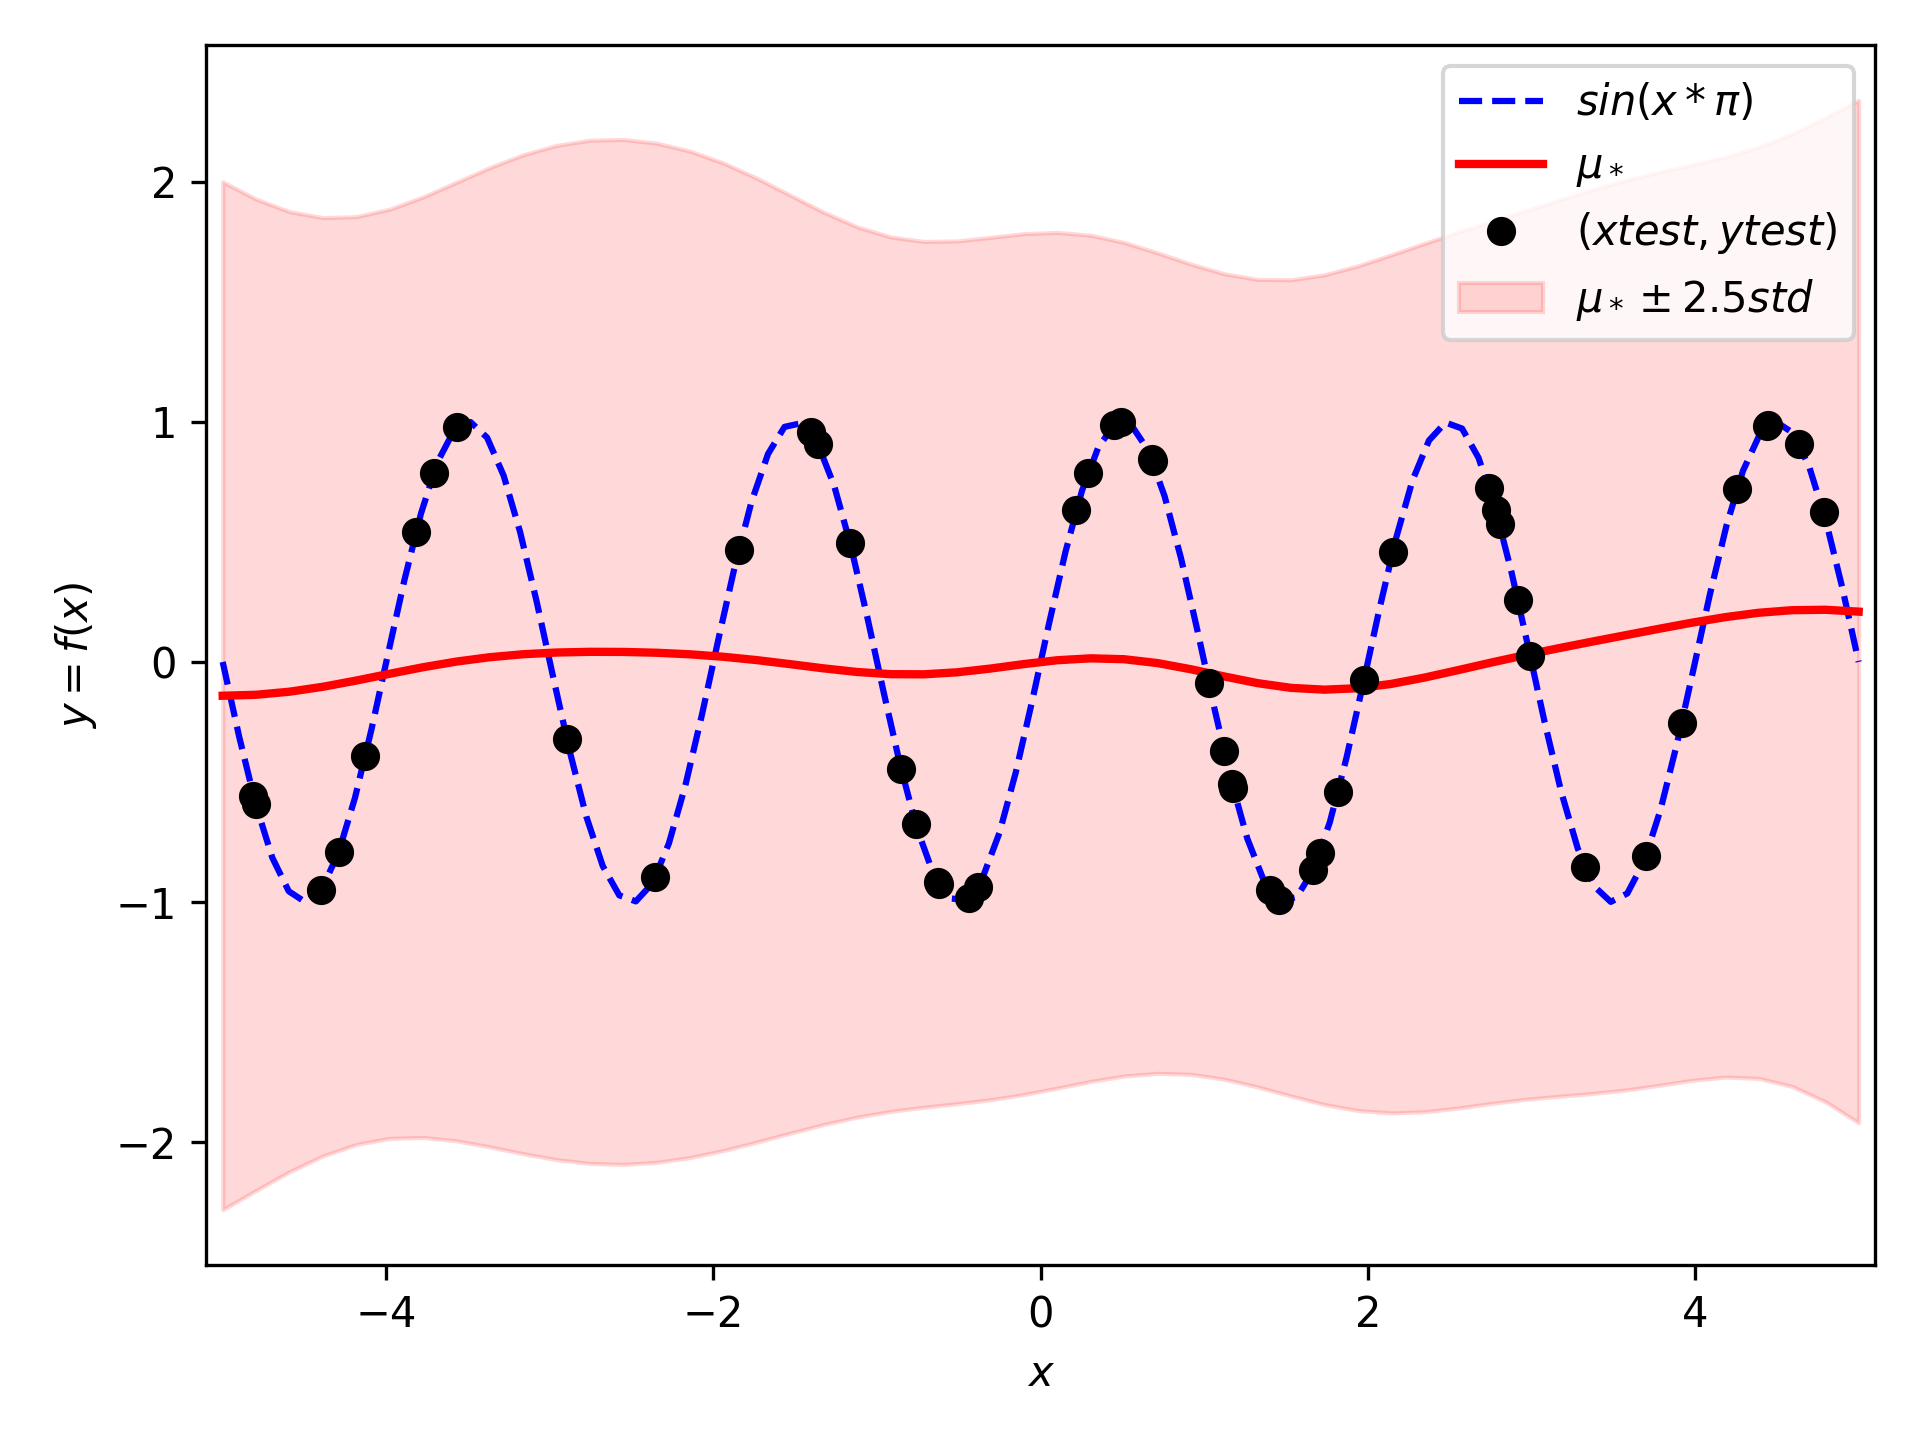
\includegraphics[width=\linewidth]{kernelSE/noise/10.png}
    \caption{$\sigma_y^2 = 10$}
    \label{fig:noise10}
  \end{subfigure}
  \caption{Gaussian Processes with SE kernel with different values of $\sigma_y^2$. The remaining parameters of SE kernel are fixed ($\ell = 1$ and $\sigma = 1$).}
  \label{fig:noise}
\end{figure}


\subsection{Effect of kernel function}

Here, we evaluate effects of different kernel functions on the GP model and on our predictions, without optimizing their hyperparameters that were kept at their default. All experiments in this section used 50 samples in the training and test sets, using the function sine as the target function. 

First, we plotted some samples of the priors of each kernel function (SE, OU, RQ and ESS kernels), without noise in the observations, in Fig. \ref{fig:priors}. When we choose a different kernel function, we are changing the shape of the functions priors, that will be conditioned by our training data with some uncertainty about it. We also plotted some functions sampled from the prior, but with noise in the observations ($\sigma_y^2 = 0.01$), in Fig. \ref{fig:noisy_priors}. Then, the curve becomes more wiggly when the noise is added to the priors. Finally, we note that both SE and RQ kernels are more rounded, and the OU and ESS are less rounded, which is expected for the kernel functions. In addition, we also observe that the ESS kernel is periodic, which is also expected.

\begin{figure}[ht]
  \begin{subfigure}{.245\textwidth}
    \centering
    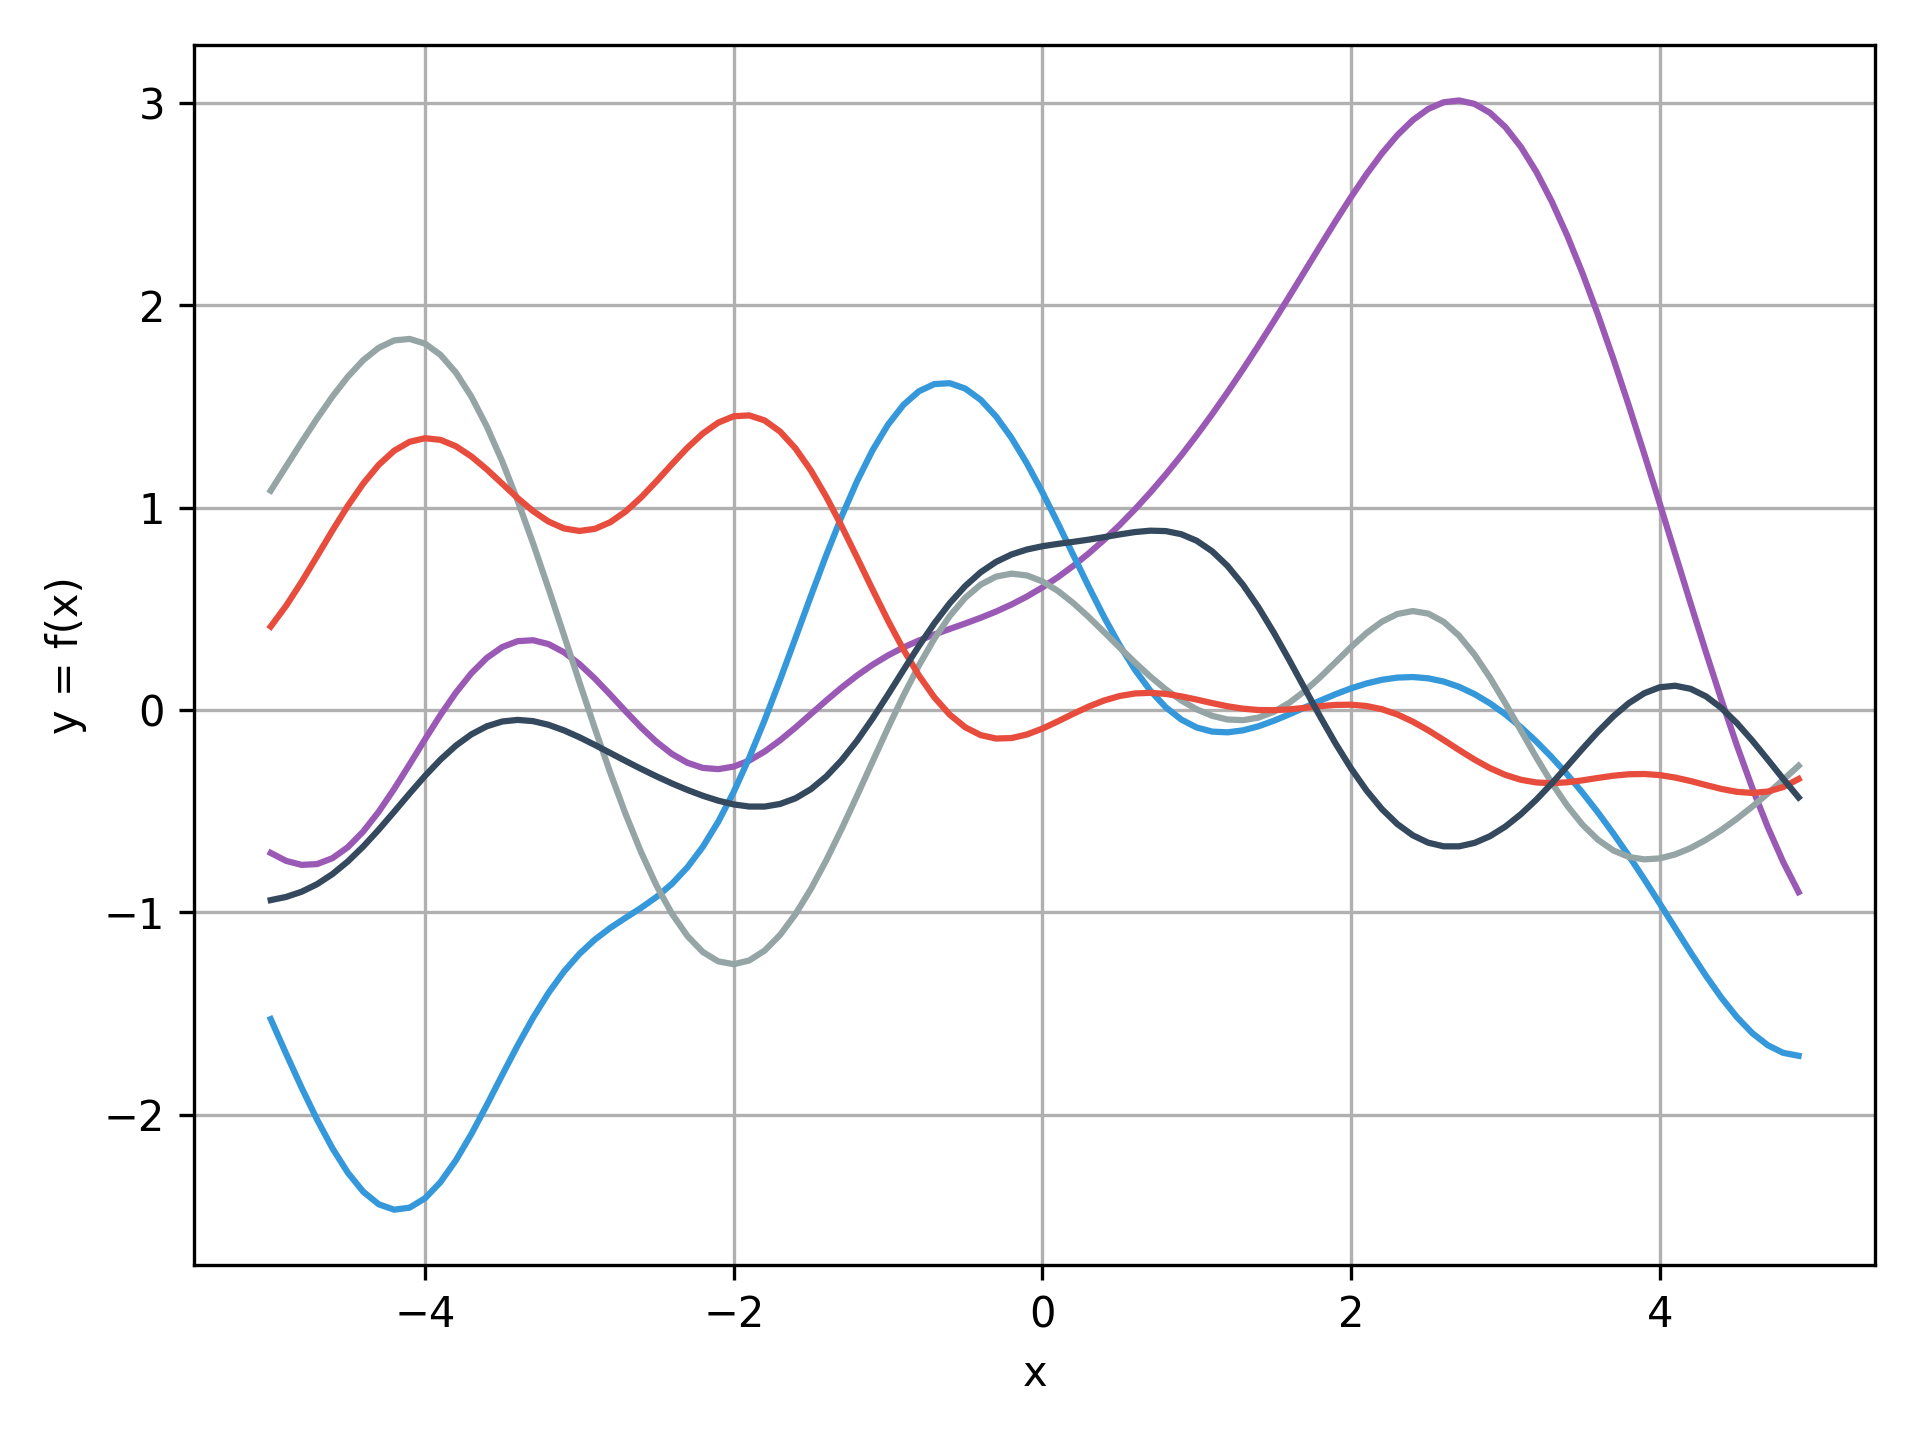
\includegraphics[width=\linewidth]{kernels/prior/noise-free/kernelSE.png}
    \caption{SE kernel}
    \label{fig:priorSE}
  \end{subfigure}
  \begin{subfigure}{.245\textwidth}
    \centering
    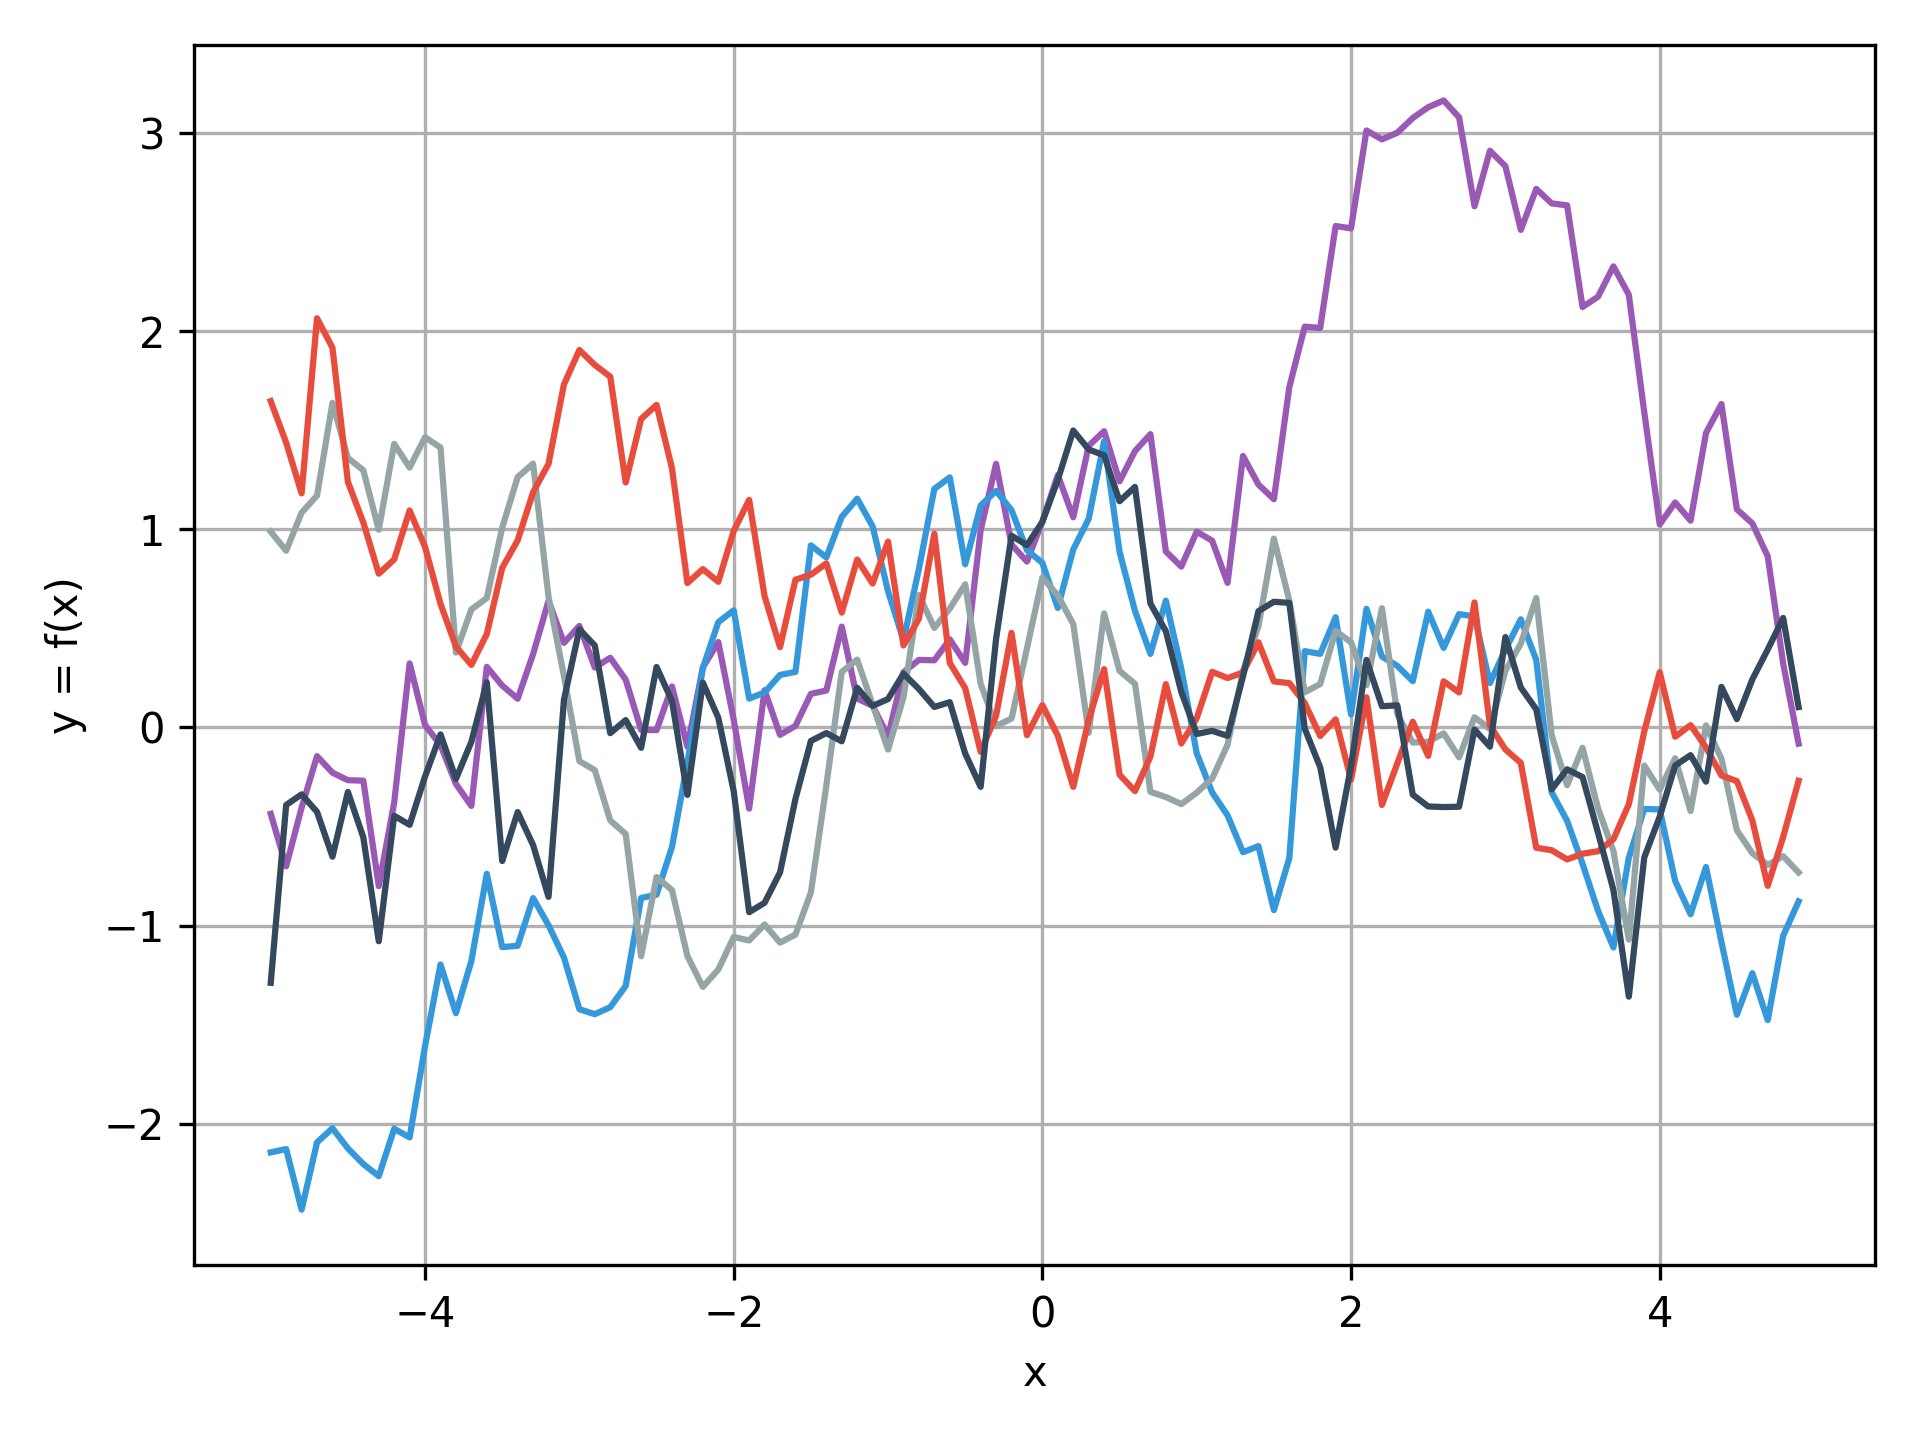
\includegraphics[width=\linewidth]{kernels/prior/noise-free/kernelOU.png}
    \caption{OU kernel}
    \label{fig:priorOU}
  \end{subfigure}
  \begin{subfigure}{.245\textwidth}
    \centering
    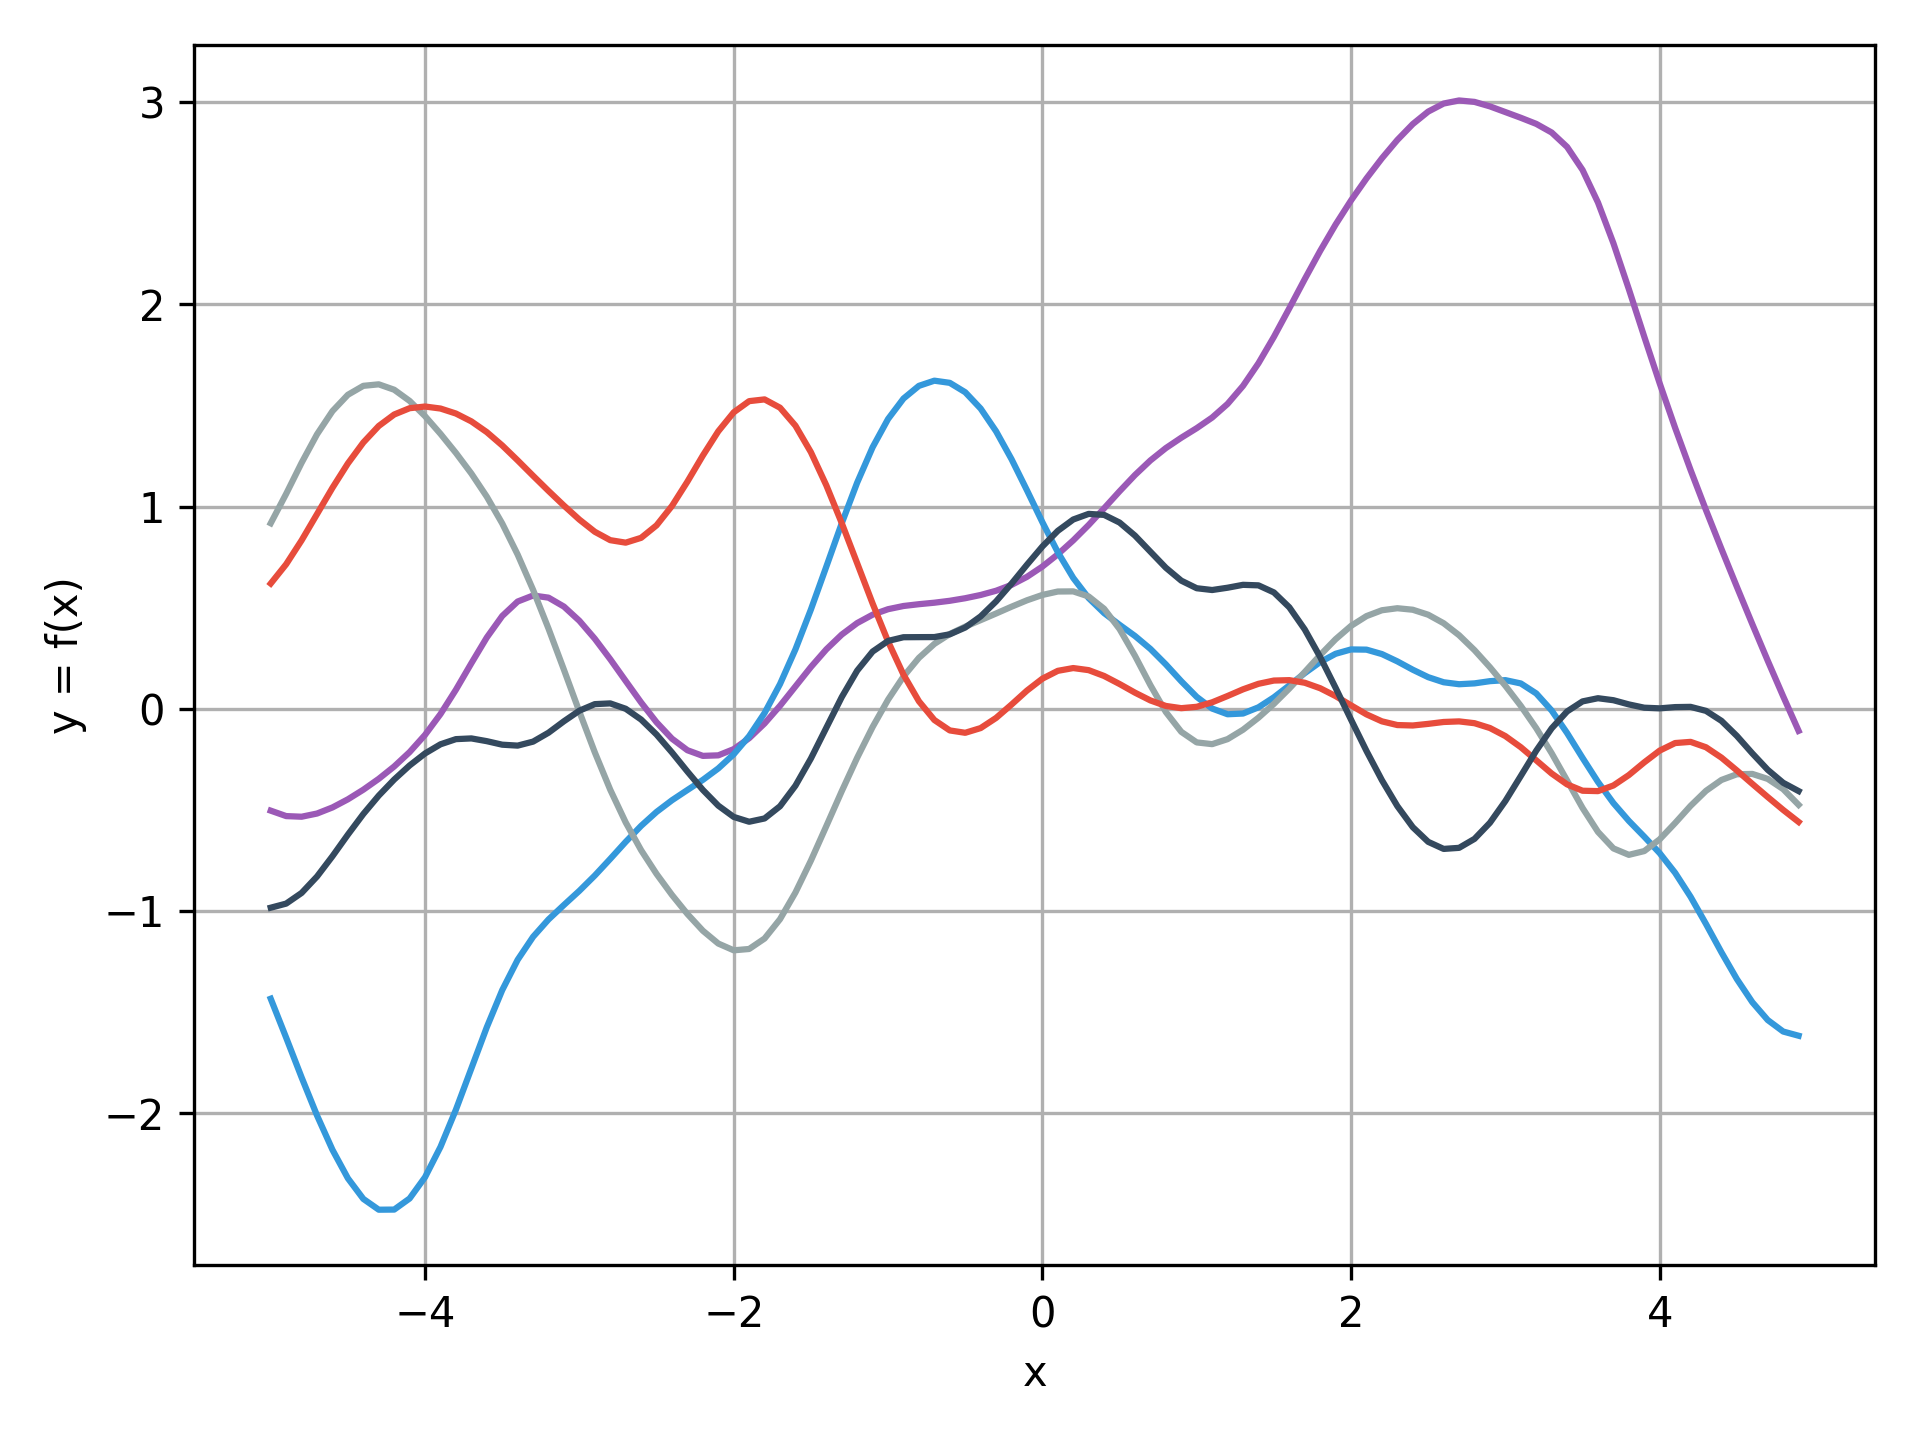
\includegraphics[width=\linewidth]{kernels/prior/noise-free/kernelRQ.png}
    \caption{RQ kernel}
    \label{fig:priorRQ}
  \end{subfigure}
  \begin{subfigure}{.245\textwidth}
    \centering
    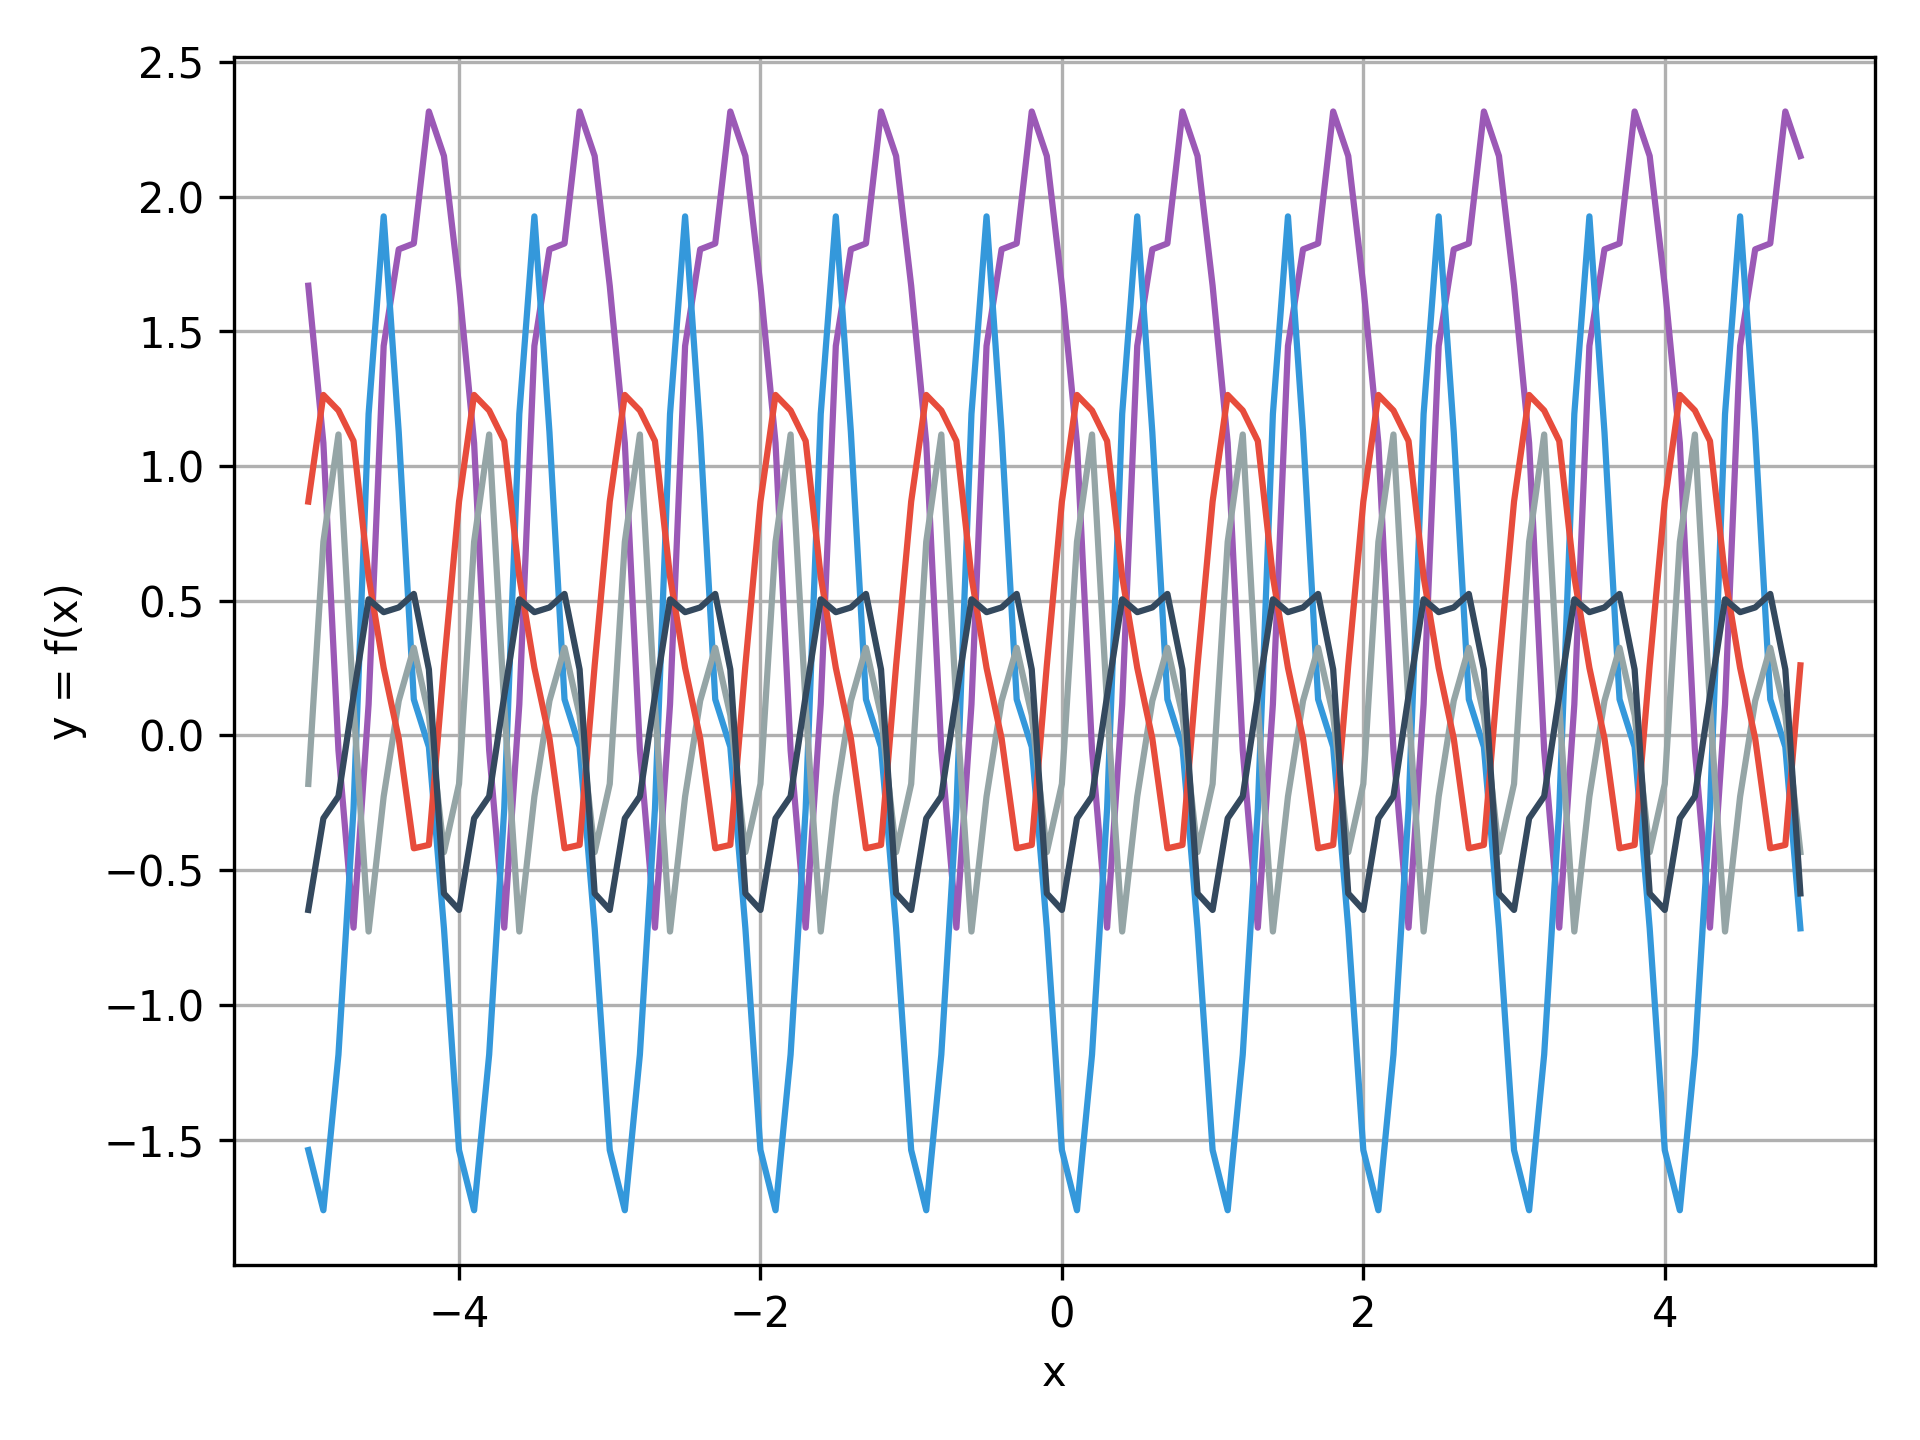
\includegraphics[width=\linewidth]{kernels/prior/noise-free/kernelESS.png}
    \caption{ESS kernel}
    \label{fig:priorESS}
  \end{subfigure}
  \caption{Five function sampled from a GP prior without noise with different kernels.}
  \label{fig:priors}
\end{figure}

\begin{figure}[ht]
  \begin{subfigure}{.245\textwidth}
    \centering
    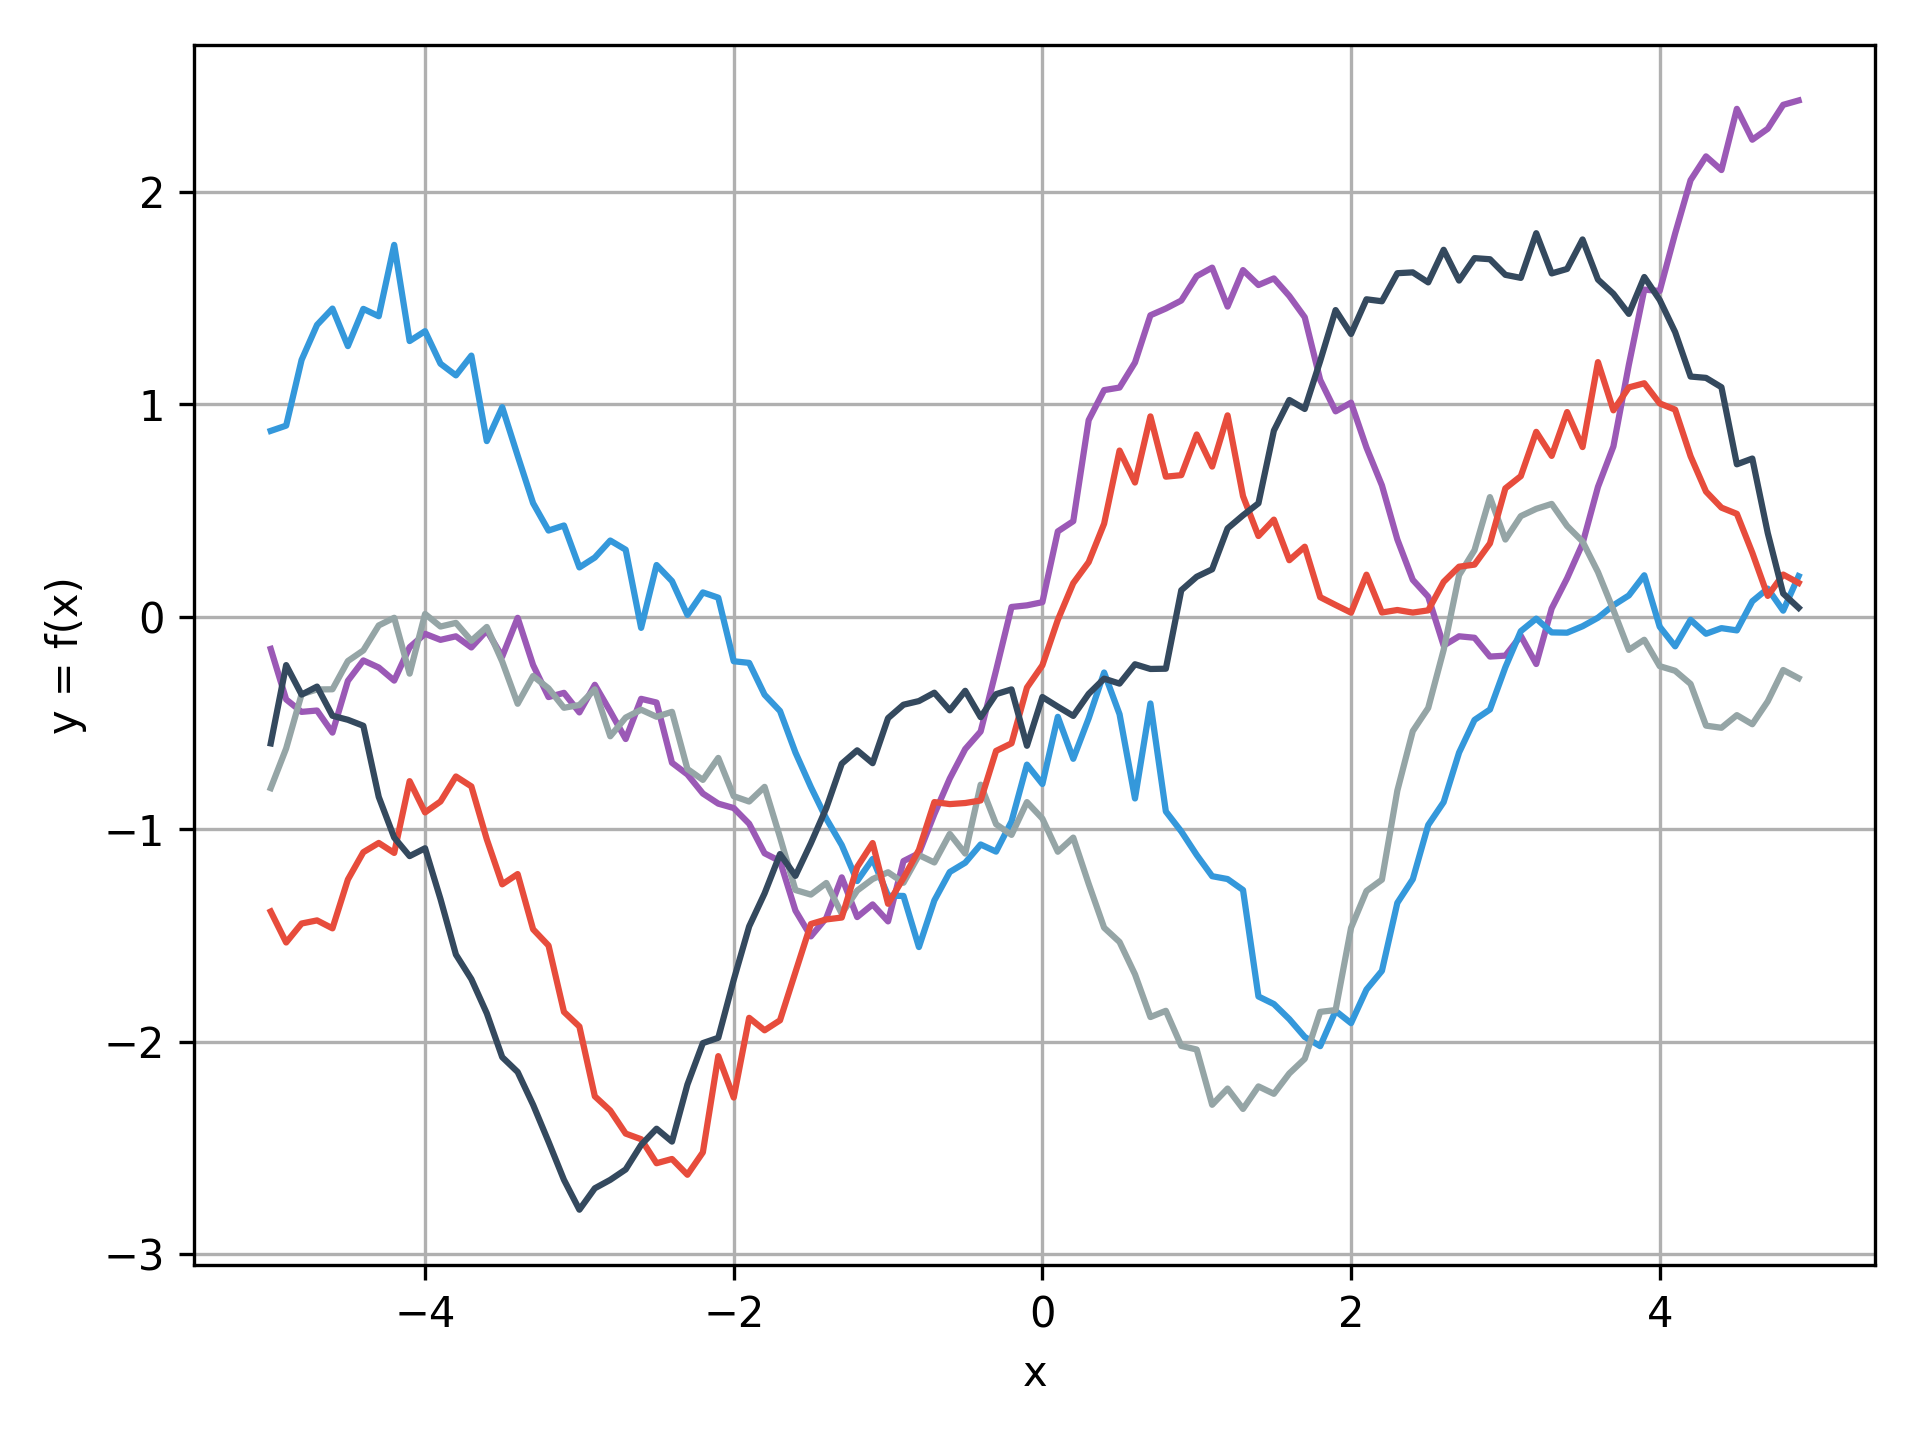
\includegraphics[width=\linewidth]{kernels/prior/noisy/kernelSE.png}
    \caption{SE kernel}
    \label{fig:priorSE}
  \end{subfigure}
  \begin{subfigure}{.245\textwidth}
    \centering
    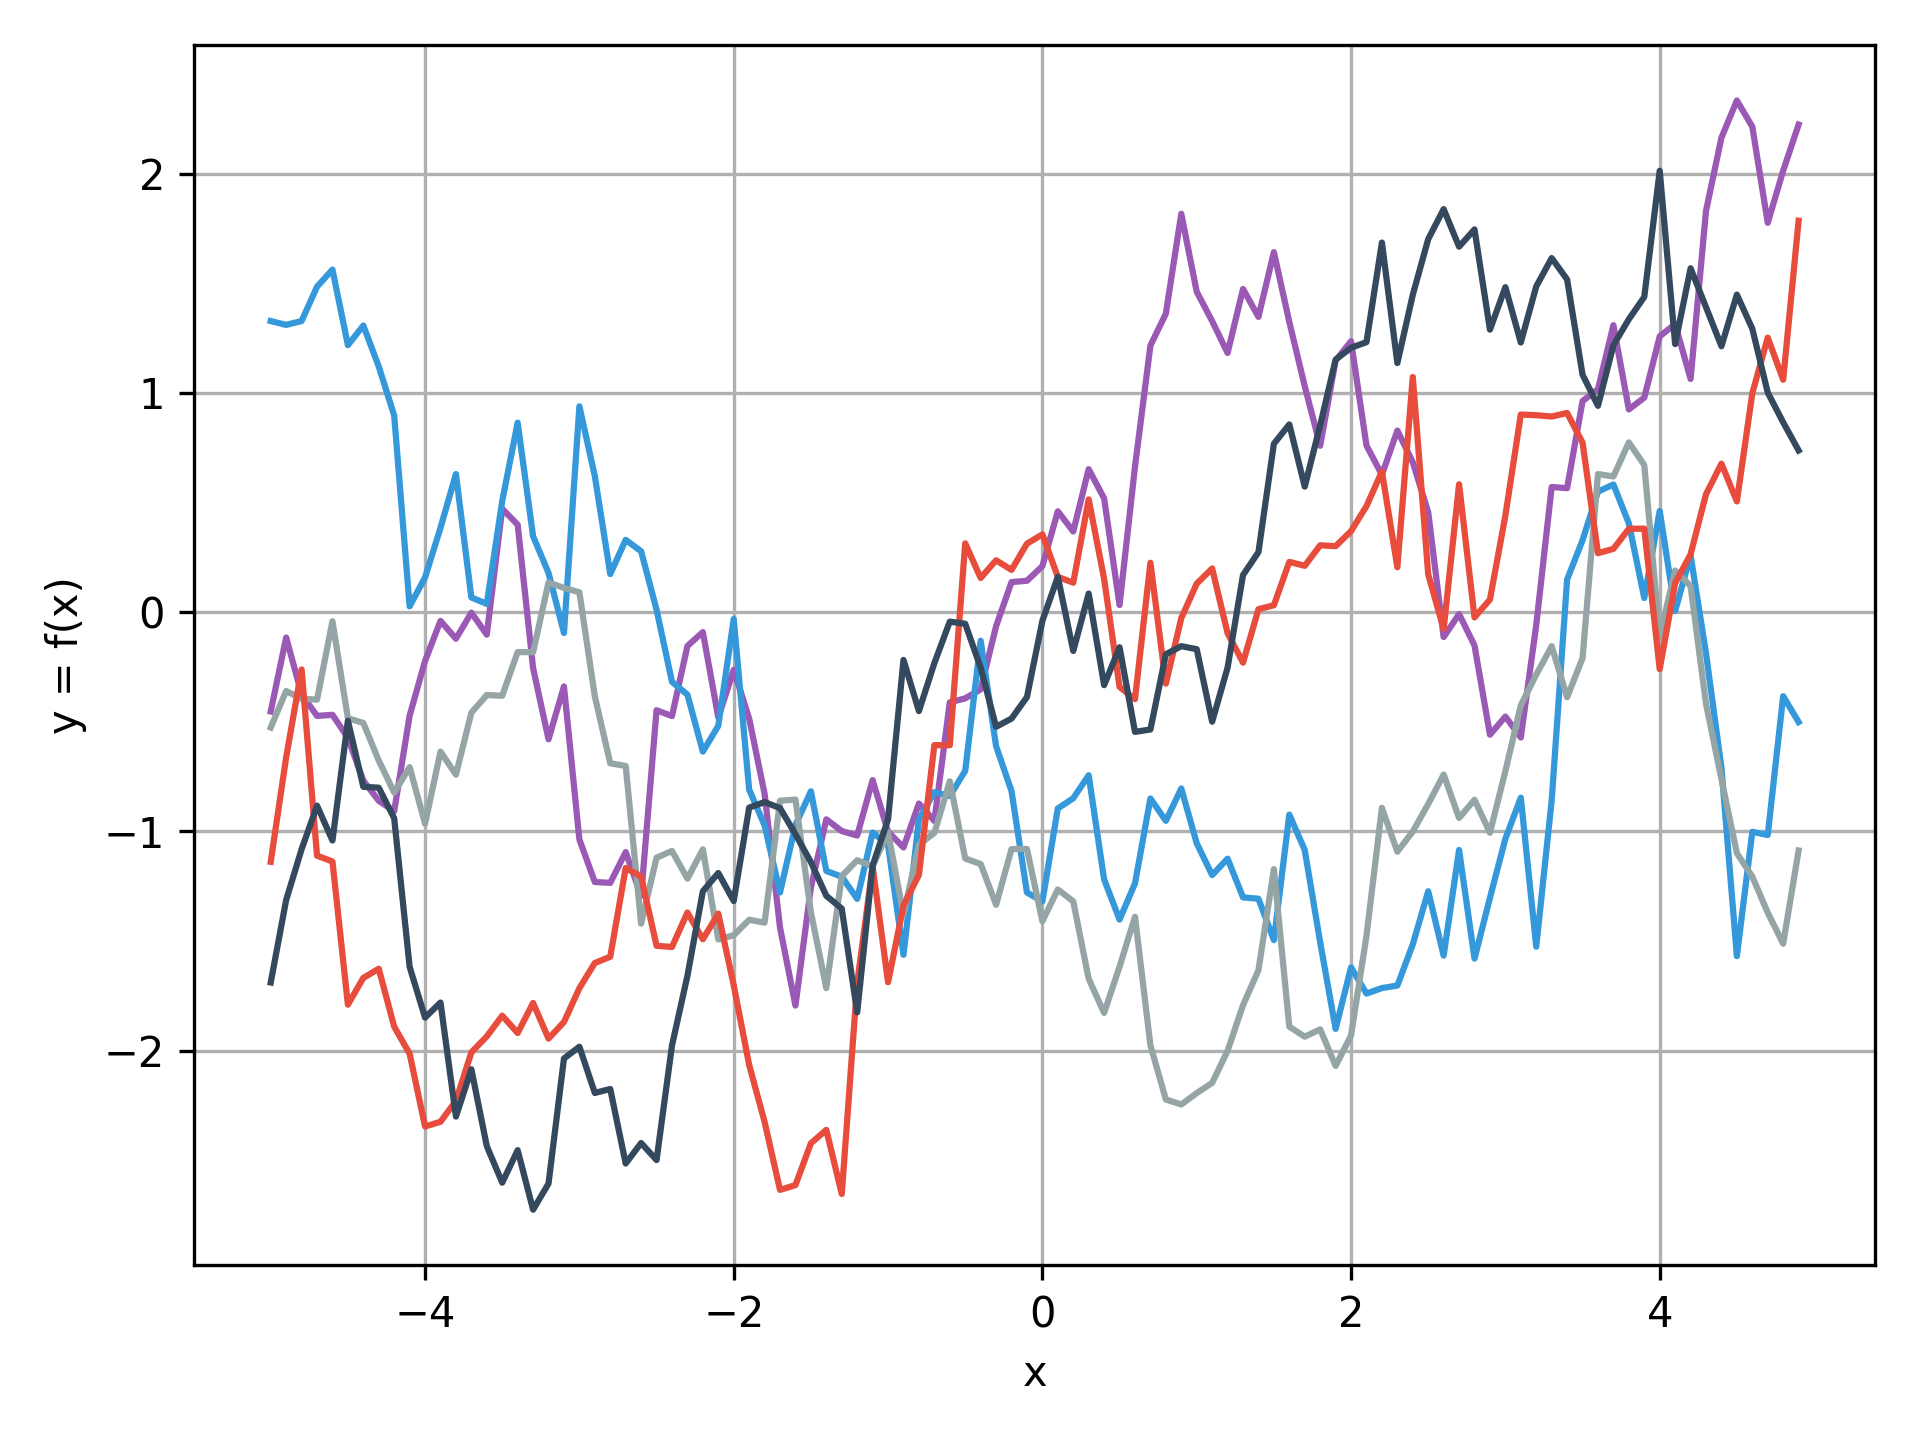
\includegraphics[width=\linewidth]{kernels/prior/noisy/kernelOU.png}
    \caption{OU kernel}
    \label{fig:priorOU}
  \end{subfigure}
  \begin{subfigure}{.245\textwidth}
    \centering
    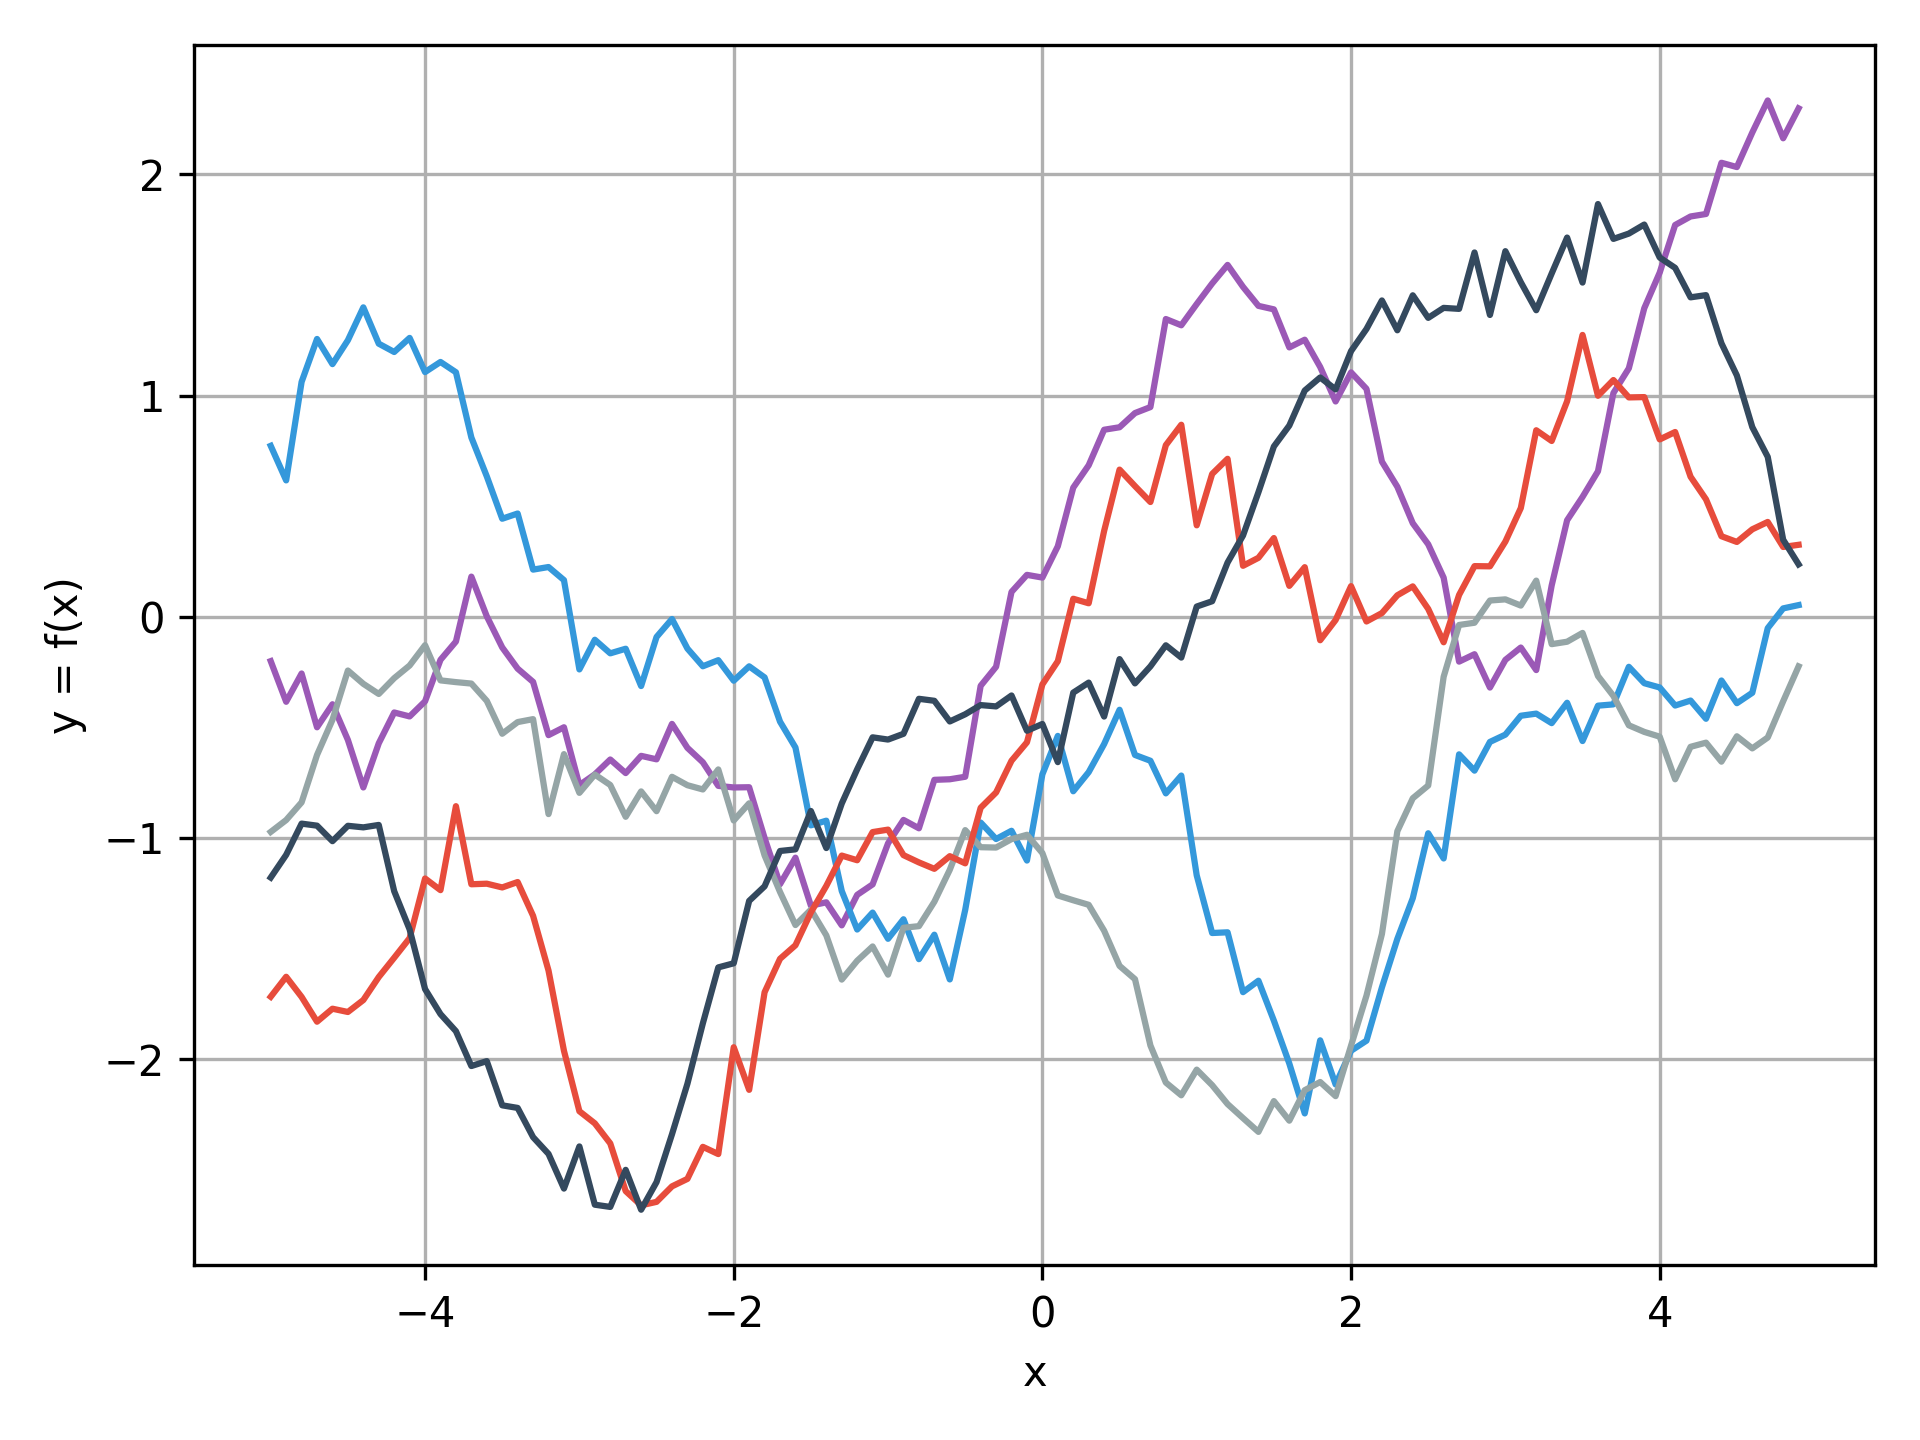
\includegraphics[width=\linewidth]{kernels/prior/noisy/kernelRQ.png}
    \caption{RQ kernel}
    \label{fig:priorRQ}
  \end{subfigure}
  \begin{subfigure}{.245\textwidth}
    \centering
    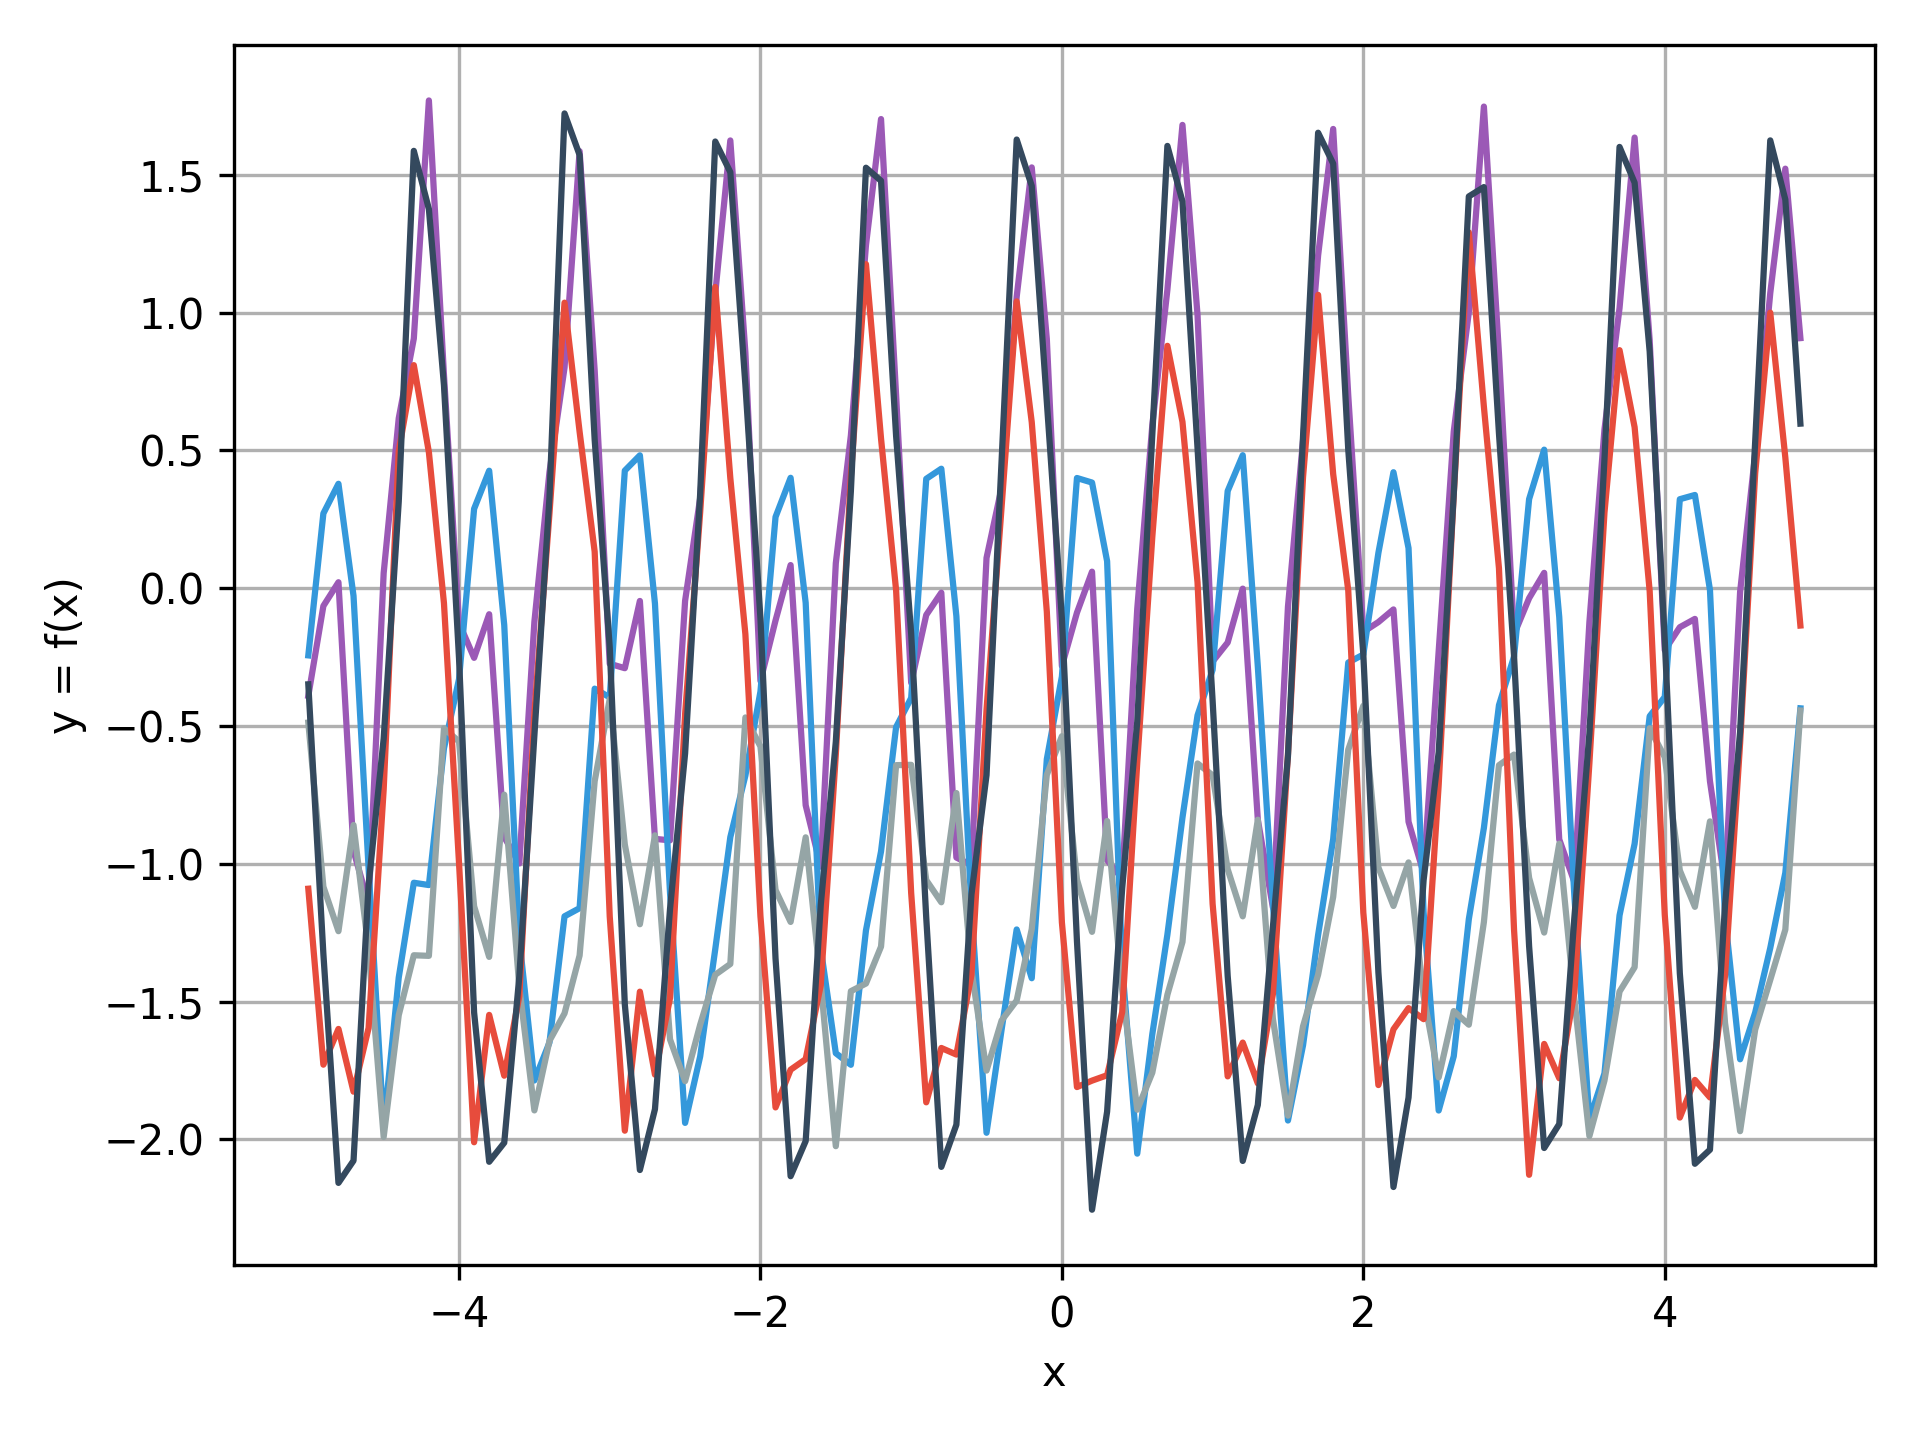
\includegraphics[width=\linewidth]{kernels/prior/noisy/kernelESS.png}
    \caption{ESS kernel}
    \label{fig:priorESS}
  \end{subfigure}
  \caption{Five function sampled from a GP prior with noise ($\sigma_y^2 = 0.01$) with different kernels.}
  \label{fig:noisy_priors}
\end{figure}

Then, we plotted the GP posteriors with noisy observations ($\sigma_y^2 = 0.01$) in Fig. \ref{fig:posterior_kernels}. Based on results, we noted that the RQ kernel (Fig. \ref{fig:kernelRQ50}), followed by the SE kernel (Fig. \ref{fig:kernelSE50}), presented the best fit to our target function, and the ESS kernel (Fig. \ref{fig:kernelESS50}) presented the worst fit. However, the hyperparameters were not optimized and therefore, we are not able to define the best kernel function to our target function without further experiments.

% All kernels posterior
\begin{figure}[ht]
  \begin{subfigure}{.5\textwidth}
    \centering
    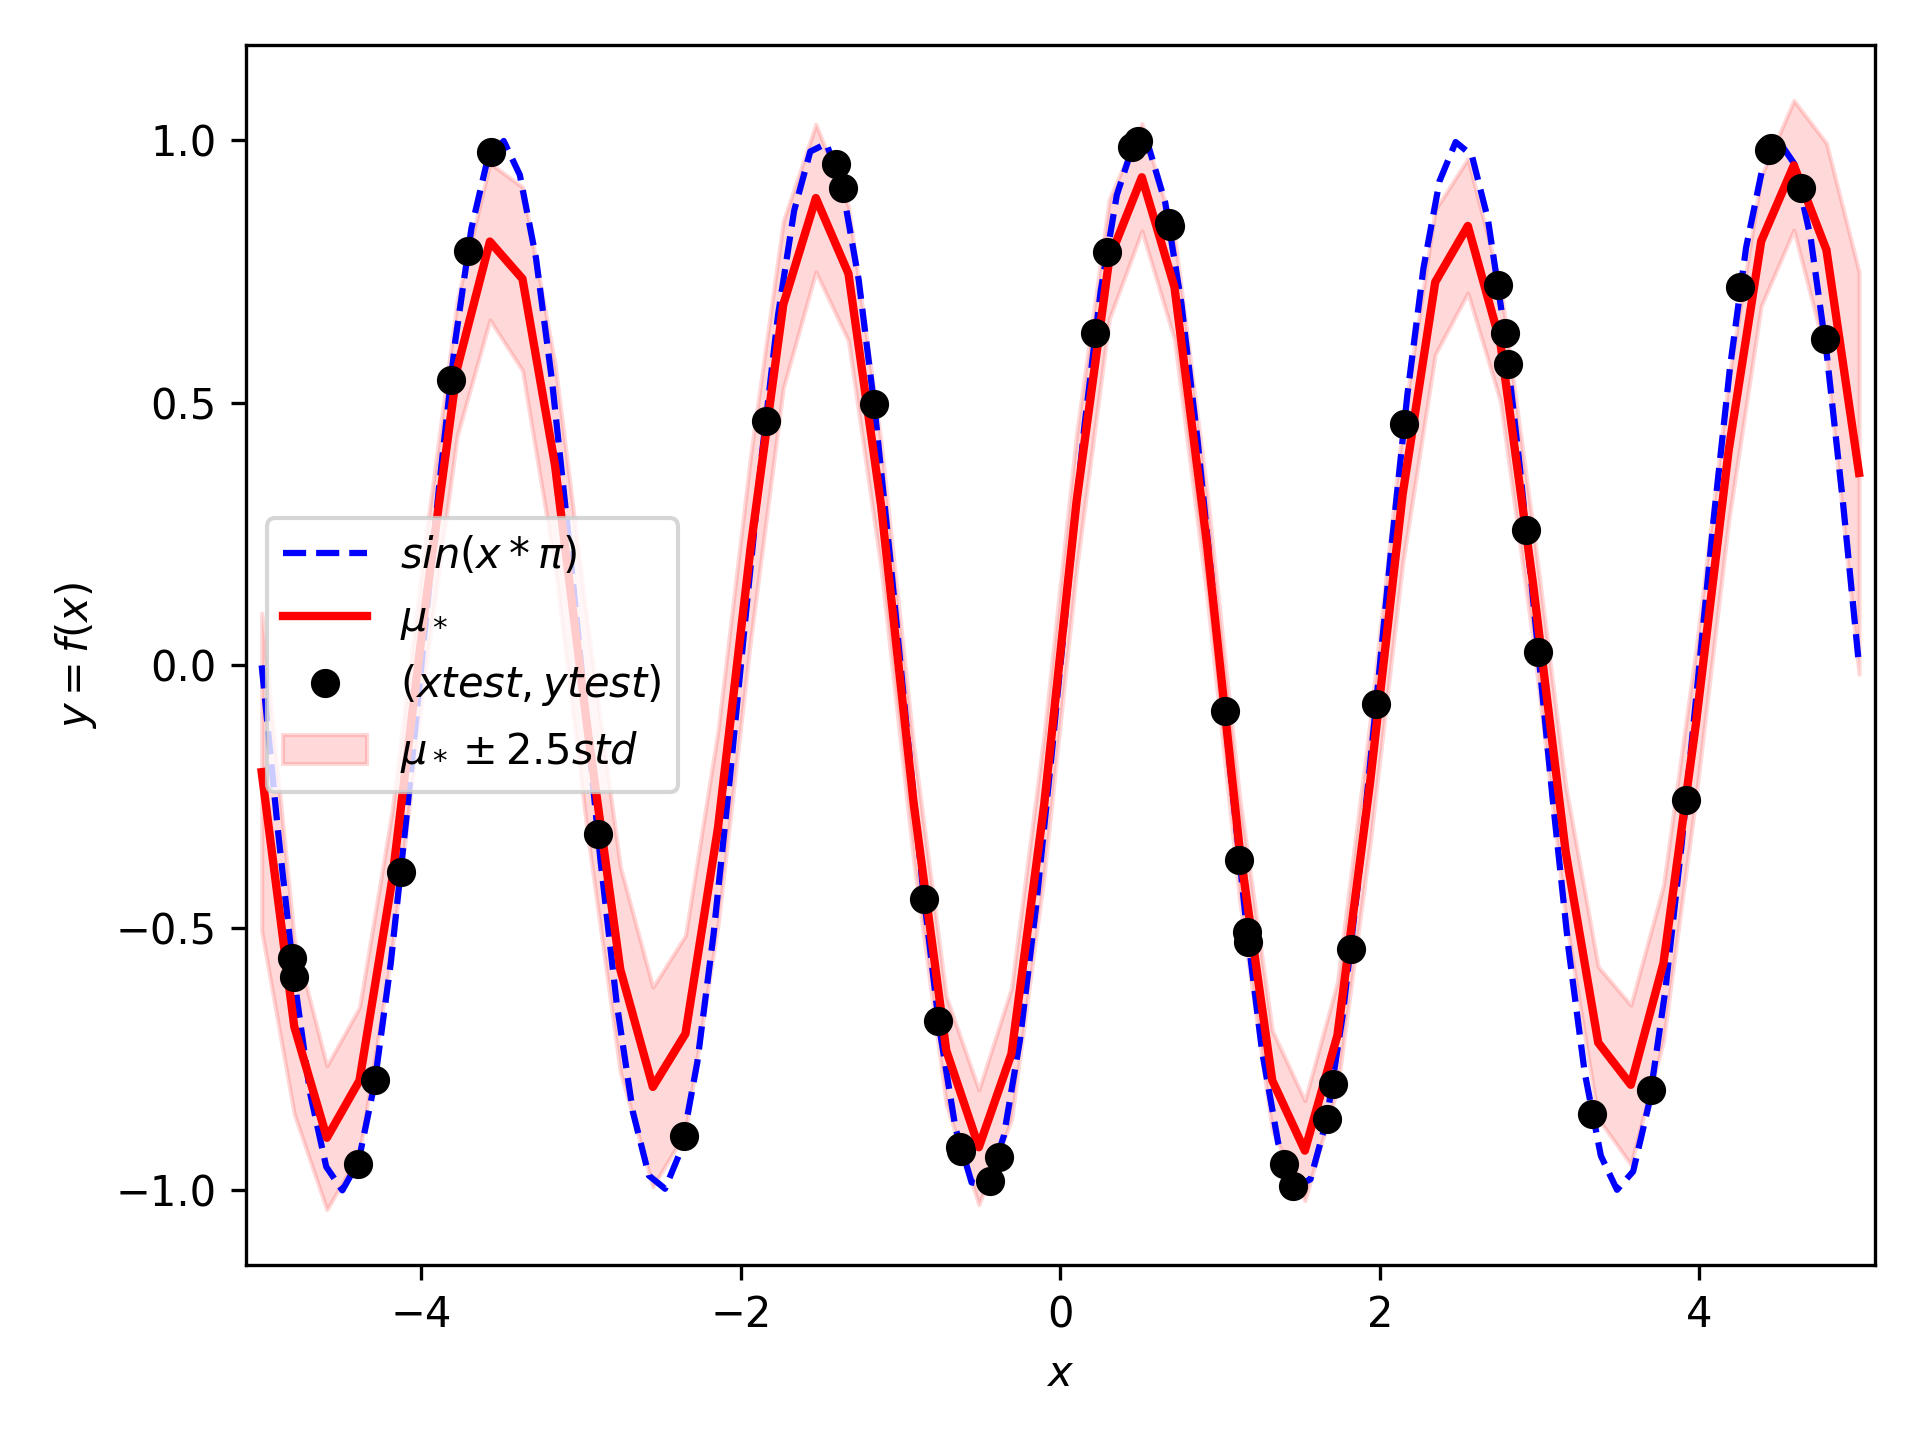
\includegraphics[width=\linewidth]{kernels/posterior/kernelSE.png}
    \caption{SE kernel}
    \label{fig:kernelSE50}
  \end{subfigure}
  \begin{subfigure}{.5\textwidth}
    \centering
    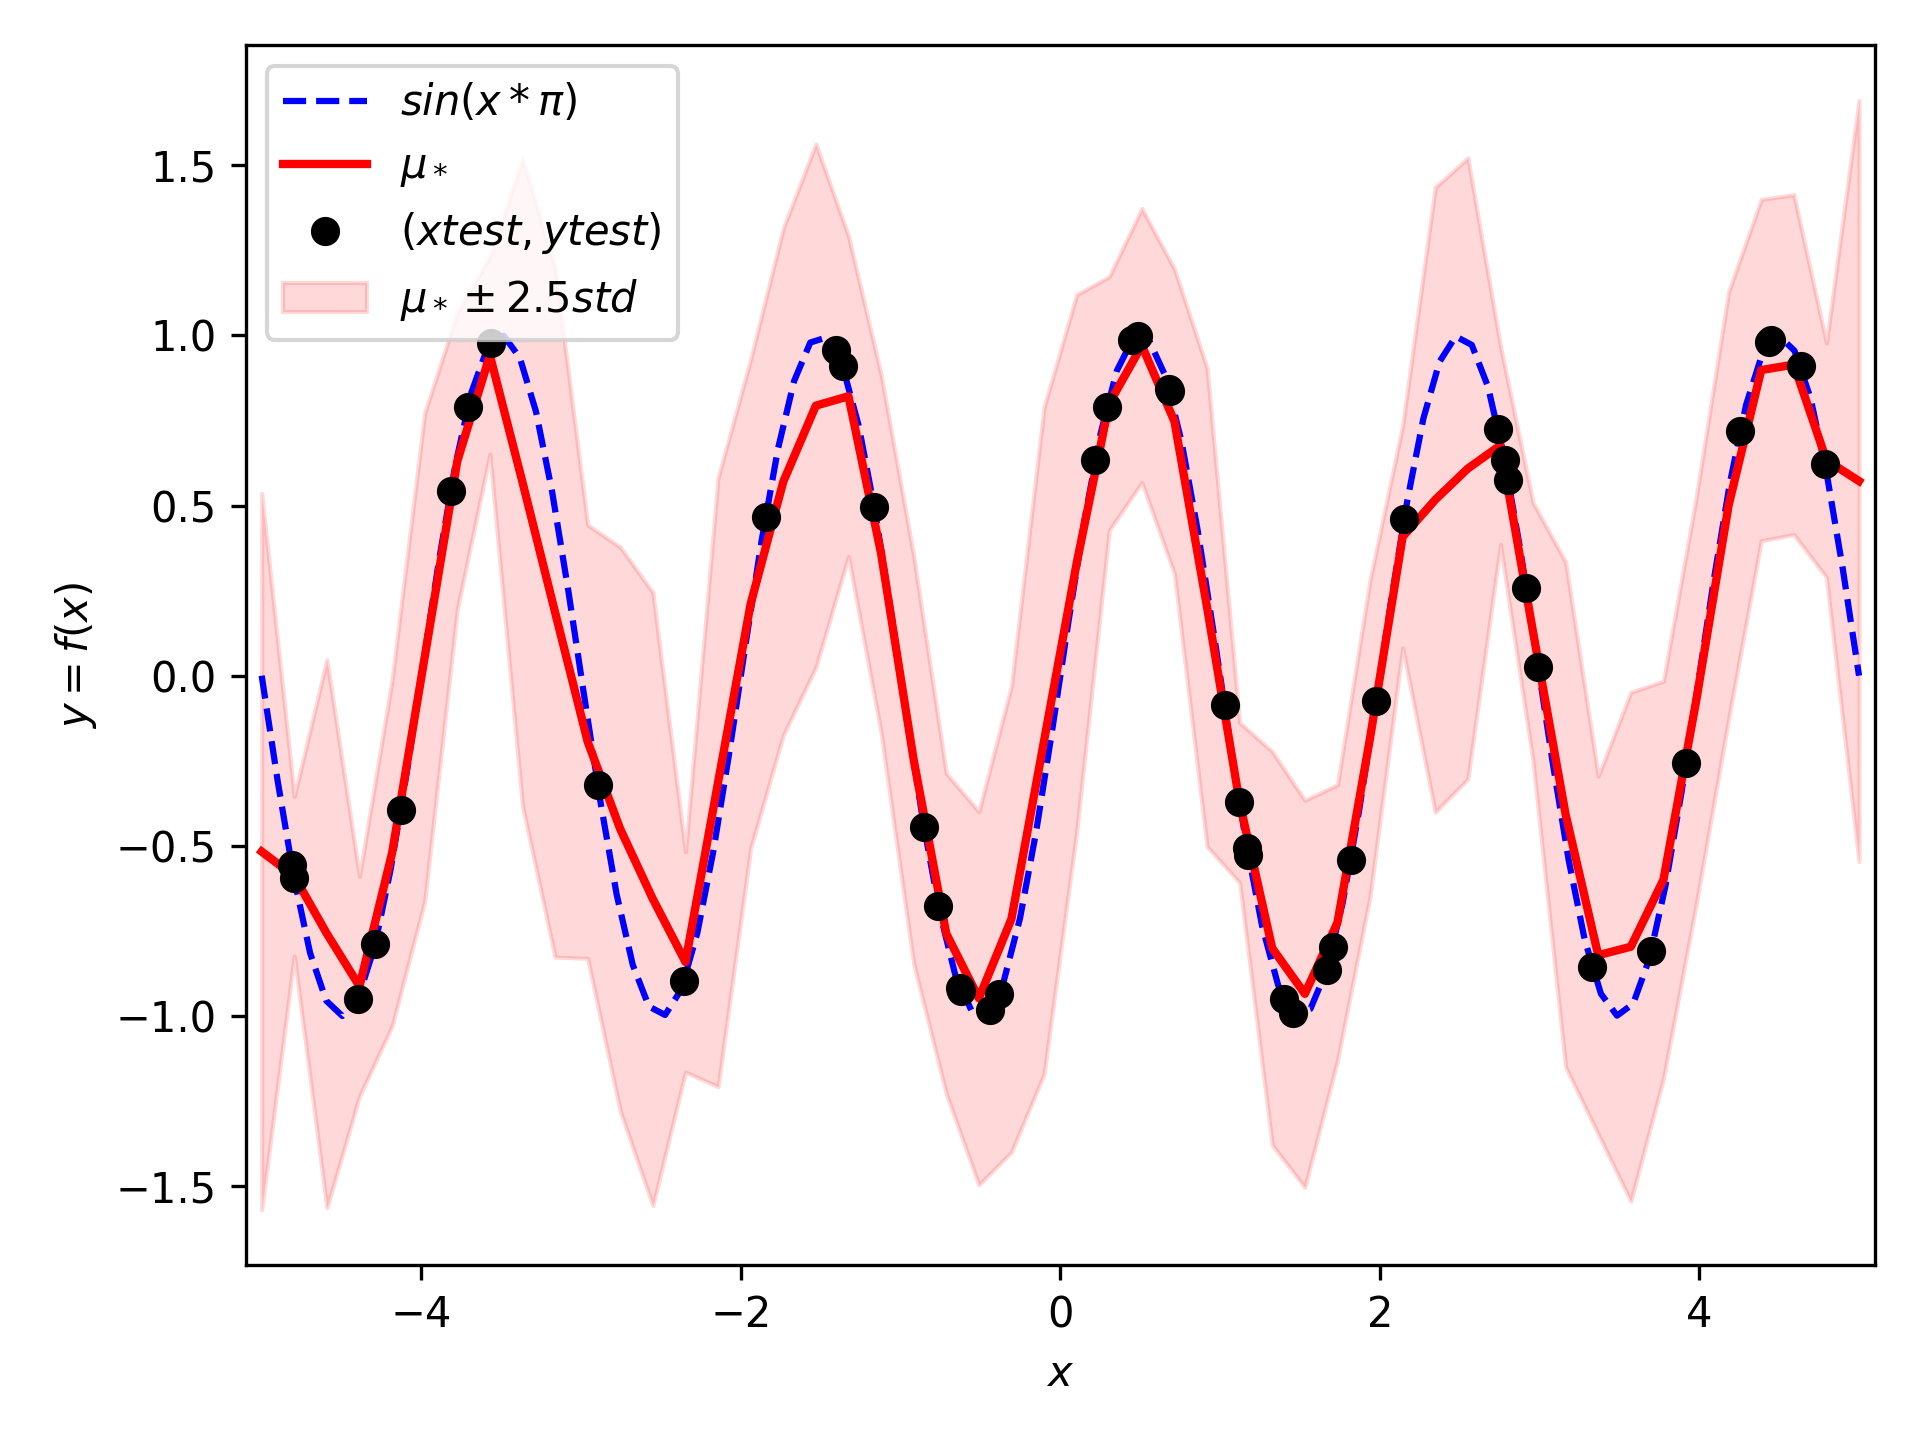
\includegraphics[width=\linewidth]{kernels/posterior/kernelOU.png}
    \caption{OU kernel }
    \label{fig:kernelOU50}
  \end{subfigure}
  \begin{subfigure}{.5\textwidth}
    \centering
    \includegraphics[width=\linewidth]{kernels/posterior/kernelRQ.png}
    \caption{RQ kernel}
    \label{fig:kernelRQ50}
  \end{subfigure}
  \begin{subfigure}{.5\textwidth}
    \centering
    \includegraphics[width=\linewidth]{kernels/posterior/kernelESS.png}
    \caption{ESS kernel}
    \label{fig:kernelESS50}
  \end{subfigure}
  \caption{Gaussian Processes with different kernel. The parameters of each kernel are: $\kappa_{SE} = \{\sigma=1.0, \ell=1.0\}$, $\kappa_{OU} = \{\sigma=1.0, \ell=1.0\}$, $\kappa_{RQ} = \{\sigma=1.0, \ell=1.0, \alpha=1.0\}$ and $\kappa_{ESS} = \{\sigma=1.0, \ell=1.0, w=1.0\}$.}
  \label{fig:posterior_kernels}
\end{figure}

Hence, the key ideia of the choice of the kernel function is to determine almost all the generalization properties of the GP model. So, it is an essential step to choose correctly the kernel function to be employed in the problem, as it has a large effect on the results.

\subsection{Predictions with higher dimensional data}

Previously, we successfully predict functions based on our one-dimensional data. To illustrate our model ability to predict in higher dimensional data, we sampled 100 training points from a 2D periodic function (Eq.\eqref{eq:2d}), and we used 900 test points to to predict a mean 2D function (Fig. \ref{fig:GP2D}).

\begin{figure}
  \centering
  \includegraphics[width=\linewidth]{GP2D/posterior.png}
  \caption{2D Gaussian Processes with multi-dimensional SE kernel.}
  \label{fig:GP2D}
\end{figure}

Comparing Fig. \ref{fig:1}d and Fig. \ref{fig:GP2D}, we notice that our mean function has not a good fit for our target function. It is worth mentioning that we used much more data points in the 2D GP than in the 1D GP, and we had a worse prediction. Then, we suggest that in higher dimensions, the GP is less sensitive to the increase in sample size. Due to limitation on computational resources, we did not perform the prediction with more points in the training and test sets. However, we are able to apply our algorithm in higher dimensional data.

\section{Conclusion}

In this project, we sucessfully implemented a Gaussian Process algorithm for regression, and evaluated the effects of the parameters and hyperparameters on the predictions. First, the number of samples on the training and test sets directly affects the quality of the predictions. Next, the hyperparameters (\eg $\sigma$, $\ell$ and $\sigma_y^2$) also affects the quality of the predictions, but each has a different effect on the predicted function. Hence, the hyperparameters should be optimized to achieve the best predictions possible. In addition, different kernel functions define functions with different shapes, that are conditioned by the training data on the GP posterior. Finally, our algorithm can be employed on higher dimensional data.
 
\printbibliography

\end{document}